%%%%%%%%%%%%%%%%%%%%%%%%%%%%%%%%%%%%%%%%%
% Masters/Doctoral Thesis 
% LaTeX Template
% Version 1.43 (17/5/14)
%
% This template has been downloaded from:
% http://www.LaTeXTemplates.com
%
% Original authors:
% Steven Gunn 
% http://users.ecs.soton.ac.uk/srg/softwaretools/document/templates/
% and
% Sunil Patel
% http://www.sunilpatel.co.uk/thesis-template/
%
% License:
% CC BY-NC-SA 3.0 (http://creativecommons.org/licenses/by-nc-sa/3.0/)
%
% Note:
% Make sure to edit document variables in the Thesis.cls file
%
%%%%%%%%%%%%%%%%%%%%%%%%%%%%%%%%%%%%%%%%% 

%----------------------------------------------------------------------------------------
%	PACKAGES AND OTHER DOCUMENT CONFIGURATIONS
%----------------------------------------------------------------------------------------

\documentclass[11pt, oneside]{Thesis} % The default font size and one-sided printing (no margin offsets)

\graphicspath{{Pictures/}} % Specifies the directory where pictures are stored
%\usepackage{apacite}
\usepackage[comma, sort&compress]{natbib} % Use the natbib reference package - read up on this to edit the reference style; if you want text (e.g. Smith et al., 2012) for the in-text references (instead of numbers), remove 'numbers' 

%\usepackage{booktabs}
%\usepackage{array}
\usepackage{amsmath,array}
\newcolumntype{L}[1]{>{\raggedright\arraybackslash}m{#1}}
%\usepackage{apacite}
\usepackage{multirow}
\usepackage{fixltx2e}
\usepackage{enumerate}
\usepackage{enumitem}
\usepackage{bibentry}
\usepackage{pdfpages}
\def\SPSB#1#2{\rlap{\textsuperscript{\textcolor{red}{#1}}}\SB{#2}}
\def\SP#1{\textsuperscript{\textcolor{black}{#1}}}
\def\SB#1{\textsubscript{\textcolor{black}{#1}}}
\newenvironment{myquote}
               {\list{}{\rightmargin   \leftmargin
                        \parsep        0in }%
                \item\relax}
               {\endlist}
\newcommand{\userquote}[2]{\begin{samepage}\begin{myquote} 
     \em{\small{#2\begin{flushright}---#1\end{flushright}}}
   \end{myquote}
   \end{samepage}}
\newcolumntype{x}[1]
            {>{\raggedright}p{#1}}
\newcommand{\tn}{\tabularnewline}

\hypersetup{urlcolor=blue, colorlinks=true} % Colors hyperlinks in blue - change to black if annoying
\title{\ttitle} % Defines the thesis title - don't touch this

\begin{document}
\bibpunct[, ]{(}{)}{;}{a}{,}{,} 
\frontmatter % Use roman page numbering style (i, ii, iii, iv...) for the pre-content pages

\setstretch{1.3} % Line spacing of 1.3

% Define the page headers using the FancyHdr package and set up for one-sided printing
\fancyhead{} % Clears all page headers and footers
\rhead{\thepage} % Sets the right side header to show the page number
\lhead{} % Clears the left side page header

\pagestyle{fancy} % Finally, use the "fancy" page style to implement the FancyHdr headers

\newcommand{\HRule}{\rule{\linewidth}{0.5mm}} % New command to make the lines in the title page

% PDF meta-data
\hypersetup{pdftitle={\ttitle}}
\hypersetup{pdfsubject=\subjectname}
\hypersetup{pdfauthor=\authornames}
\hypersetup{pdfkeywords=\keywordnames}

%----------------------------------------------------------------------------------------
%	TITLE PAGE
%----------------------------------------------------------------------------------------

\begin{titlepage}
\begin{center}

\textsc{\LARGE \univname}\\[1.5cm] % University name
\textsc{\Large Doctoral Thesis}\\[0.5cm] % Thesis type

\HRule \\[0.5cm] % Horizontal line
{\huge \bfseries \ttitle}\\[0.4cm] % Thesis title
\HRule \\[1.5cm] % Horizontal line

\begin{minipage}{0.4\textwidth}
\begin{flushleft} \large
\emph{Author:}\\
{\authornames} % Author name - remove the \href bracket to remove the link
\end{flushleft}
\end{minipage}
\begin{minipage}{0.4\textwidth}
\begin{flushright} \large
\emph{Supervisors:} \\
{\supname} % Supervisor name - remove the \href bracket to remove the link  
\end{flushright}
\end{minipage}\\[3cm]
 
\large \textit{A thesis submitted in fulfilment of the requirements\\ for the degree of \degreename}\\[0.3cm] % University requirement text
\textit{in the}\\[0.4cm]
\groupname\\\deptname\\[2cm] % Research group name and department name
 
{\large \today}\\[4cm] % Date
%
\includegraphics{Logo} % University/department logo - uncomment to place it
 
\vfill
\end{center}

\end{titlepage}

%----------------------------------------------------------------------------------------
%	DECLARATION PAGE
%	Your institution may give you a different text to place here
%----------------------------------------------------------------------------------------

\Declaration{

\addtocontents{toc}{\vspace{1em}} % Add a gap in the Contents, for aesthetics

I, \authornames, declare that this thesis titled, '\ttitle' and the work presented in it are my own. I confirm that:

\begin{itemize} 
\item[\tiny{$\blacksquare$}] This work was done wholly or mainly while in candidature for a research degree at this University.
\item[\tiny{$\blacksquare$}] Where any part of this thesis has previously been submitted for a degree or any other qualification at this University or any other institution, this has been clearly stated.
\item[\tiny{$\blacksquare$}] Where I have consulted the published work of others, this is always clearly attributed.
\item[\tiny{$\blacksquare$}] Where I have quoted from the work of others, the source is always given. With the exception of such quotations, this thesis is entirely my own work.
\item[\tiny{$\blacksquare$}] I have acknowledged all main sources of help.
\item[\tiny{$\blacksquare$}] Where the thesis is based on work done by myself jointly with others, I have made clear exactly what was done by others and what I have contributed myself.\\
\end{itemize}
 
Signed:\\
\rule[1em]{25em}{0.5pt} % This prints a line for the signature
 
Date:\\
\rule[1em]{25em}{0.5pt} % This prints a line to write the date
}

\clearpage % Start a new page

%----------------------------------------------------------------------------------------
%	QUOTATION PAGE
%----------------------------------------------------------------------------------------

\pagestyle{empty} % No headers or footers for the following pages

\null\vfill % Add some space to move the quote down the page a bit

\textit{``Education is what remains after one has forgotten what one has learned in school.''}

\begin{flushright}
Albert Einstein
\end{flushright}

\vfill\vfill\vfill\vfill\vfill\vfill\null % Add some space at the bottom to position the quote just right

\clearpage % Start a new page

%----------------------------------------------------------------------------------------
%	ABSTRACT PAGE
%----------------------------------------------------------------------------------------

\addtotoc{Abstract} % Add the "Abstract" page entry to the Contents

\abstract{\addtocontents{toc}{\vspace{1em}} % Add a gap in the Contents, for aesthetics
There is an increasing prevalence of chronic diseases that are associated with living unhealthy lifestyle in both developed and developing world contexts. In order to help combat this unfavourable trend, public health researchers are advocating towards shifting care to the hands of citizens through utilization of personalized interventions . The objective of these initiatives is to support individuals beyond the point of care. ICTs, specifically mobile phones coupled with sophisticated persuasive mechanisms such as gamification or simple strategies such as SMS reminders provide an opportune platform for delivery of personalized interventions that target health behaviour change. In order to support delivery of such personalized interventions, researchers in human-computer interaction have developed an area of research referred to as personal informatics, which focuses on data collection and feedback mechanisms. These approaches aim at supporting individuals to be able to quantify different aspects of their lives through self-reflection. These systems have been developed with motivational affordance to sustain their utilization by end users. However, such systems are developed with only one user in mind of which is a direct user of technology. Such systems may not scale well in contexts of indirect users of technology, meaning people who use technology through a facilitation of a human interface (intermediary user) situated between indirect users (beneficiaries of technology) and technology. Therefore, there was a need to explore how motivational affordance of a personal health informatics could be extended to work in the context of an interaction that requires a collaboration that leads to indirect usage. This was a collaboration between the person helping and the person being helped.

In order to understand design implications for indirect technology use in the context of a personal health informatics, several approaches were used to understand social dynamics that could affect utilization of technology through a human interface in between indirect users and technology. Prototypes of mobile self monitoring applications for physical activity and diet were developed and used as the starting point for uncovering unknown issues. As the result of evaluation of the aforementioned prototypes , the researcher suggested both social technical arrangements and prerequisites that increase the likelihood of success in utilization of such interventions. 

One of the important social technical arrangement was a prior social relationship between a human interface and a beneficiary of technology through a human interface. Self-determination theory was used to understand how motivation for collaboration between the two sets of users (the human interface and beneficiary user of technology ) could be enhanced. Gamification, a design pattern inspired by games  was found to be the source of a significant increase in perceived competence, an aspect of self-determination theory. Therefore, gamification was found to be a catalyst for increasing collaboration between a human interface and beneficiary user of technology provided that the two users that form a pair had a prior social relationship. The collaborative gamified system showed promising results towards utilization of personal health informatics in the context of indirect usage. The most promising combination of a human interface and beneficiary user is the one that entails family members, possibly a child and a parent.

Despite the success of gamification in increasing perceived competence of the human interface, and hence collaboration between a human interface and beneficiary user, there are some design implications that need to be taken into consideration in order to understand how internalization of collaboration between two members of a pair working together could be improved. This entails exploration of features that support task mastery climate versus those that support ego-involved. Future research could also explore how different styles of parenting could affect the way the intervention is perceived by the two sets of users.
}

\clearpage % Start a new page

%----------------------------------------------------------------------------------------
%	ACKNOWLEDGEMENTS
%----------------------------------------------------------------------------------------

\setstretch{1.3} % Reset the line-spacing to 1.3 for body text (if it has changed)

\acknowledgements{\addtocontents{toc}{\vspace{1em}} % Add a gap in the Contents, for aesthetics
The first people I am grateful to are my research supervisors for their guidance and encouragement during PhD journey; Dr Melissa Densmore and Prof. Ulrike Rivett. I thank them for believing in me. I would also like to extend my acknowledgement to the Late Prof. Gary Marsden (R.I.P) who was my main supervisor before his demise. Through him that is where I started to build the passion for human-computer interaction. He was more that just a supervisor. I would like to also acknowledge his widow, Gil Marsden together with her two children for hosting us at their home as Gary's students.

Also I would like to thank HPI Research School and Centre of Excellence both at UCT for their generous scholarship, and travel and research grants that were very instrumental in facilitation of my PhD journey. My acknowledgement are extended Memalani NGO in Cape Town who played a role in recruitment of participants at some stage of role. In additional to Mamelani, special acknowledgement goes to Minah Radebe of Langa in  Cape Town and her field worker who were both very instrumental in assisting towards recruitment of participants and facilitation of evaluation in general.

The acknowledgements extend to all my fellow students at ICT4D Lab -- University of Cape Town (UCT) whom within their presence the lab was not only an academic environment but a large social support group. To mention for individuals, special acknowledgement goes to Christopher Chepken, Raymond Mughwanya, Grace Ssekakubo, Richard Ssembatya, Mvurya Mgala, Thomas Reitmaier, and many more whose names I have not mentioned here but I appreciate their contribution. Also special acknowledgements goes to the ICOMMS research group of which I was part of. I would also like to pass my acknowledgement are my country mates at University Cape Town who made my stay in Cape Town appear like a home far from home.   

I also acknowledge Craig Balfour, a system administrator at the department for his technical support on the infrastructure for hosting the application online. Special thanks also goes Eve Gill, the financial administrator at the Department of Computer Science for being effective in processing funds whenever they were required. 


Last but not least, my gratitude is to my wife (Lulu) and son (Lucas) for their patience during this challenging but rewarding journey.   
}
\clearpage % Start a new page

%----------------------------------------------------------------------------------------
%	LIST OF CONTENTS/FIGURES/TABLES PAGES
%----------------------------------------------------------------------------------------

\pagestyle{fancy} % The page style headers have been "empty" all this time, now use the "fancy" headers as defined before to bring them back

\lhead{\emph{Contents}} % Set the left side page header to "Contents"
\tableofcontents % Write out the Table of Contents

\lhead{\emph{List of Figures}} % Set the left side page header to "List of Figures"
\listoffigures % Write out the List of Figures

\lhead{\emph{List of Tables}} % Set the left side page header to "List of Tables"
\listoftables % Write out the List of Tables

%----------------------------------------------------------------------------------------
%	ABBREVIATIONS
%----------------------------------------------------------------------------------------

\clearpage % Start a new page

\setstretch{1.5} % Set the line spacing to 1.5, this makes the following tables easier to read

\lhead{\emph{Abbreviations}} % Set the left side page header to "Abbreviations"
\listofsymbols{ll} % Include a list of Abbreviations (a table of two columns)
{
\textbf{BBM} & \textbf{B}lack \textbf{B}erry \textbf{M}essenger \\
\textbf{BMI} & \textbf{B}ody \textbf{M}ass \textbf{I}ndex \\
\textbf{CHW} & \textbf{C}ommunity \textbf{H}ealth \textbf{W}orkers\\
\textbf{GPS} & \textbf{G}lobal \textbf{P}ositioning \textbf{S}ystem\\
\textbf{HCI} & \textbf{H}uman \textbf{C}omputer \textbf{I}nteraction\\
\textbf{ICT} & \textbf{I}nformation and \textbf{C}ommunications \textbf{T}echnology \\
\textbf{ICTD} & \textbf{I}nformation and \textbf{C}ommunications \textbf{T}echnology and \textbf{D}evelopment\\
\textbf{MMS} & \textbf{M}ultimedia \textbf{M}essaging \textbf{S}ervice\\
\textbf{NEAT} & \textbf{N}on-\textbf{E}xercise \textbf{A}ctivity \textbf{T}hermogenesis\\
\textbf{PDA} & \textbf{P}ersonal \textbf{D}igital \textbf{A}ssistant\\
\textbf{PSD} & \textbf{P}ersuasive \textbf{S}ystem \textbf{D}esign\\
\textbf{RCT} & \textbf{R}andomized \textbf{C}ontrolled \textbf{T}rial\\
\textbf{SIM} & \textbf{S}ubscriber \textbf{I}dentity \textbf{M}odule \\
\textbf{SMS} & \textbf{S}hort \textbf{M}essaging \textbf{S}ervice \\
\textbf{USSD} & \textbf{U}nstructured \textbf{S}upplementary \textbf{S}ervice \textbf{D}ata \\
\textbf{URL} & \textbf{U}niform \textbf{R}esource \textbf{L}ocator\\
%\textbf{Acronym} & \textbf{W}hat (it) \textbf{S}tands \textbf{F}or \\
}

%----------------------------------------------------------------------------------------
%	DEDICATION
%----------------------------------------------------------------------------------------
\clearpage % Start a new page
\setstretch{1.3} % Return the line spacing back to 1.3

\pagestyle{empty} % Page style needs to be empty for this page

\dedicatory{This work is dedicated to my great parents, my father, Andalwisye, and my late mother, Mary for supporting me throughout my academic journey.} % Dedication text




%\addtocontents{toc}{\vspace{2em}} % Add a gap in the Contents, for aesthetics
 %----------------------------------------------------------------------------------------
%	PUBLICATIONS
%----------------------------------------------------------------------------------------
\clearpage % Start a new page

\setstretch{1.5} % Set the line spacing to 1.5, this makes the following tables easier to read

\lhead{\emph{List of Publications}} % Set the left side page header to "Abbreviations"
\listofpubs % Include a list of Abbreviations (a table of two columns)
{
\nobibliography*
%\bibliographystyle{unsrt}
  \section*{List of Publications}
  \begin{enumerate}
    \item \bibentry{katule2016leveraging}
    \item \bibentry{katule2016family}
  \end{enumerate}
}
\addtocontents{toc}{\vspace{2em}} % Add a gap in the Contents, for aesthetics

%----------------------------------------------------------------------------------------
%	THESIS CONTENT - CHAPTERS
%----------------------------------------------------------------------------------------

\mainmatter % Begin numeric (1,2,3...) page numbering

\pagestyle{fancy} % Return the page headers back to the "fancy" style

% Include the chapters of the thesis as separate files from the Chapters folder
% Uncomment the lines as you write the chapters
% Chapter 1

\chapter{Introduction} % Main chapter title

\label{introductionchapter} % For referencing the chapter elsewhere, use \ref{Chapter1} 

%\lhead{Chapter 1. \emph{Introduction}} % This is for the header on each page - perhaps a shortened title
\lhead{Chapter \ref{introductionchapter}. \emph{Introduction}} % This is for the header on each page - perhaps a shortened title

%----------------------------------------------------------------------------------------
\section{Background}
Obesity and overweight are currently global health concerns. In one systematic review, it was revealed that overweight and obesity had a tendency to be linked to an increase of incidence of several co-morbidities, for example, type 2 diabetes and other chronic conditions like cardiovascular diseases and cancer~\citep{guh2009incidence}. The number of people who are considered to be either overweight or obese stands at approximately 1.3 billion~\citep{steyn2006chronic}. A survey by~\cite{abegunde:theburden}, which included a total of 23 low-income and middle-income countries, projected a loss of US\$84 billion in economic production between 2006 and 2015 from heart disease, stroke and diabetes alone, in the absence of any significant measures put in place to intervene.

Co-morbidities that are associated with obesity are likely to inundate healthcare systems~\citep{pollak2010s}. Todate, healthcare systems have failed to optimally treat chronic conditions such as diabetes due to the lack of time for providing continuous patient care, which is essential in the management of chronic conditions~\citep{quinn2008welldoc}. Resources are insufficient to deal with an overwhelming increase in number of patients, hence there have been suggestions to move part of the care to the hands of patients~\citep{aarsand2012mobile}.~This need calls for innovative and citizen-centric  interventions to foster lifestyle changes, in order to both prevent or delay the onset of chronic conditions in populations, and support patients in self-management of chronic conditions, to reduce the burden on healthcare systems~\citep{korhonen2010personal,aarsand2012mobile,higgins2016smartphone}. There has been a growing number of initiatives by both commercial and research communities to develop mobile applications and wearable sensors that could nudge individuals to eat healthily and increase their level of physical activity~\citep{chen2014healthytogether}. Citizen-centric interventions are now possible due to advancements in hardware and software technologies, which have facilitated the creation of opportunities for automation of health self-management processes~\citep{arsand:mobile}. 

One interesting trend in both academia and industry is the use of mobile phones in health. The mobiles have become an effective means of ``just in time'' delivery of interventions that target psychological processes~\citep{hsu2014persuasive}. These devices are currently omnipresent and people carry them most of the time~\citep{mattila2008mobile}, hence their presence adds a ``kairos factor'' to the delivery of interventions that target both health promotion~\citep{pollak2010s} and persuasion~\citep{hsu2014persuasive}. Smartphone-based applications have been rapidly gaining popularity as effective tools to support delivery of personalized health information~\citep{handel2011mhealth}. One of the prevalent uses of mobile health apps is self-monitoring, to augment \emph{cognitive behaviour therapy} -- the treatment of behaviour in clinical settings~\citep{mattila2008mobile,medynskiy2010salud}. These apps facilitate the data collection of one's health parameters through inbuilt tools such as GPS and an accelerometer (body activity sensor); hence they present an innovative way of monitoring and improving both health and fitness~\citep{higgins2016smartphone}. In order for such tools to support changes in health behaviour and the promotion of a healthy lifestyle, theory-based strategies such as gamification (for enhancement of motivation), enabling self-reflection through goal setting and feedback (for improvement of self-efficacy), and SMS reminders are often applied~\citep{consolvo2009goal,cole2010text,hamari2014persuasive,hamari2014does,higgins2016smartphone}. However, such tools have limitations when they are used in specific contexts. The basis of the research problem for this study was to address the limitations inherent in the developing world context but these limitations can as well scale to a context of developed world. The research problem is as reported below.
\section{Statement of the Problem}
A review by~\cite{higgins2016smartphone} presented evidence that self-monitoring apps can help patients reach their health and fitness goals.~These apps can also support individuals who are not patients to become aware of their behaviours, which is an important step towards taking actions that are necessary to live a healthy lifestyle. However, such apps have limitations as they don't accommodate specific interaction modes that involve the sharing of devices and indirect usage. Such modes of interaction are prevalent and relevant in the context of the developing world, and self-monitoring applications that are designed for direct use may not replicate well in some populations of users~\citep{kaplan2006can,sambasivan2010}, especially when users face barriers to direct access of user interfaces or technology~\citep{kumar2015mobile}. Typically, self-monitoring apps utilize  specific theory-informed motivational affordances in order to enhance the engagement of end users. But such incentives have been designed only for a direct user and are not supported in a situation where there are at least two layers of users that consist of an intermediary user, who acts as a bridge for an indirect user, and the indirect (beneficiary) user of information in a self-monitoring app. Such a scenario of intermediated technology is shown in Figure \ref{figure:directVSinterm}, which is profoundly explained by~\cite{sambasivan2010} from the perspective of activity theory~\citep{kaptelinin1997activity}. In a direct interaction, a computing device or system is an object that provides specific affordances of activities that an end user can perform on the object, while in an intermediated interaction there is an additional layer of human interface: the intermediary user, responsible for translating the intents of a beneficiary user into actions, by carrying out activities on a computing device or system on behalf of an indirect user (the beneficiary user).
\begin{figure}[htbp]
  \centering
    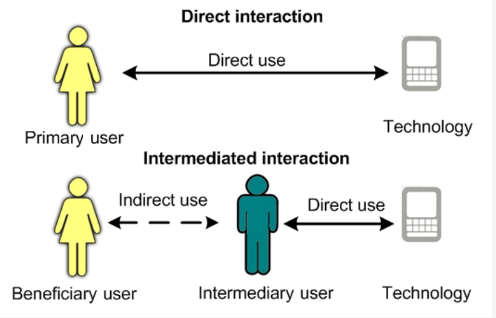
\includegraphics[width=0.6\textwidth]{Figures/intermediated.png}
    \rule{35em}{0.5pt}
  \caption{Direct and intermediated interactions~\citep{sambasivan2010}.}
  \label{figure:directVSinterm}
\end{figure}

This research explored how one could support personal health informatics technology where its usage is facilitated by intermediary users on behalf of beneficiary users (indirect users). Despite a vast amount of literature on \emph{intermediated technology use}, such persuasive technologies have not been extensively explored in this context. Persuasive technologies tend to have their unique design considerations, and intermediated technology use has its socio-technical aspects; hence one has to understand which factors to consider and how to go about implementing a useful intervention that could work in such a complex context. This study had two main research questions, as presented below.
\begin{enumerate}
%\setcounter{enumi}{1}
\item What is the role of social-technical settings in the intermediated use of gamified self-monitoring applications targeting the promotion of healthy eating and physical activity?

\textbf{Sub-questions}
\begin{enumerate}[label=\alph*.]
\item What social factors have impact on the intermediated use of a gamified self-monitoring application?
\item To what extent do those social factors affect motivation to engage with a gamified self-monitoring application in intermediated use context?
\end{enumerate}
\item How does gamification play a role in motivating the intermediated use of self-monitoring applications targeting the promotion of healthy eating and physical activity?

\textbf{Sub-questions}
\begin{enumerate}[label=\alph*.]
\item What is the impact of gamification on supporting the self-determination of intermediary users to engage with a self-monitoring application in intermediated use?
\item What is the impact of gamification on supporting the self-determination of beneficiary users to engage with a self-monitoring application in intermediated use?
\item What is the impact of gamification on the frequency of utilizing the self-monitoring application in intermediated use?
\item What is the impact of gamification on the motivation of beneficiaries to self-monitor diet?
\item What is the impact of gamification on the motivation of beneficiaries to self-monitor physical activity?
\item How does the presence of gamification affect the relationship between the two members of a pair participating in intermediated use?
\item To what extent might gamification encourage or discourage internalization of intermediated use behaviour?
\end{enumerate}
\end{enumerate}  
\section{Research Contribution}
This research grounded its findings from user evaluations, ideas from past studies and  existing theories of human motivation.~User evaluations included a total of three studies, carried out in three townships in South Africa at non-overlapping intervals of time. Each user study helped to uncover unique insights that were important in getting answers to the aforementioned research questions. Each user study consisted of several pairs of users.~Each pair of users consisted of one beneficiary user (a person who solicited help in using the self-monitoring application), and one intermediary user (a person who provided the required help to a beneficiary user: to facilitate interaction with the self-monitoring application). Beneficiary users elected their respective intermediary users and the pair had access to the app for a certain number of days before questionnaires and interviews were administered.  

Data collection techniques consisted mostly of the triangulation of the app's usage logs, interviews and questionnaires. In order to solve the problem, prior to carrying out any prototype development and evaluation, the study started with a contextual investigation to gain a preliminary understanding of users' context. The process involved administering semi-structured questionnaires to adult participants whom the research team opportunistically approached in a hospital setting in Cape Town. Iterations of software development and informative evaluations of mobile application prototypes, followed after the contextual investigation. Motivational affordances implemented on prototypes included gamification features such as leaderboards, badges, avatars, virtual pets and social interaction features.  Through the course of eliciting feedback from user studies, I as the researcher was able to generate insights in an iterative manner, where each iterative user study informed the formulation and execution of a successive user study. 

From informative evaluations, the study concluded with a summative evaluation which aimed to measure the effectiveness of using gamification in the promotion of intermediated use of self-monitoring applications. 
 
The contribution of this research is mainly to increase understanding of which social dynamics and motivational affordances to consider when designing personal health informatics (PHI) for intermediated use. In this dissertation it is suggested that rather than designing PHI for the beneficiary alone, one can design for intermediated use, explicitly acknowledging the presence of intermediary users as facilitators of access to a self-monitoring application.~This research demonstrated that it is feasible to frame the design of personal applications in a way that promotes collaboration between an intermediary user and a beneficiary user, hence reaching the goal of motivating intermediated use. The dissertation highlights some social configurations that are crucial for the intermediated use of a self-monitoring application. The dissertation further emphasizes the importance of pairing users within family settings to foster an environment that encourages intermediated use.  The study indicated that when a pair consists of immediate family members, the prior social relationship may promote internalization of help-giving behaviours on the part of intermediaries. Prior social relationship appears to be a prerequisite for setting up an intervention, and it can provide rationale for intermediaries to perceive gamification as something that is fun to use but, at the same time, as something done to support a good cause, which in this case was to help someone they care about. With the presence of that care, and by adding a gamification layer,  collaboration and family bonds show indications of improvement.~However, in some situations competition appears to harm an existing family bond between members of a pair instead of promoting it, especially when one member of a pair feels let down by the other member of the pair.~Strengths and weaknesses of different motivational affordances in terms of promoting aspects of autonomy, competence and relatedness are also discussed in detail, in order to offer insights to both designers and researchers for the design of future interventions.
\section{Thesis Organization}
I have organized this thesis as follows. Chapter 1, \emph{\textbf{Introduction}}, provides the background information of the problem, research questions, and the contribution of this research to knowledge. Chapter 2, \emph{\textbf{Literature Review}}, mainly covers  the theoretical underpinning of this research in terms of related work and the conceptual framework that lays a foundation for this research. Chapter 3 is on \emph{\textbf{Study Context}}, which situates this work in the South African context by providing a rationale for carrying out a study in South African townships. Chapter 4 presents the \emph{\textbf{Contextual Enquiry}}, which we conducted at the beginning of the study to understand how technology is being utilized in general in the context of older adults who are prospective beneficiary users of the technology. In addition, this contextual enquiry aimed to uncover whether there were particular usages of technology that were health related. Chapter 5, \emph{\textbf{Prototype I}}, describes the development and evaluation of the first prototype. In the development part, I generated the preliminary user requirements after combining insights gained from both the preliminary findings of the contextual enquiry and ideas grounded in literature. Chapter 6, \emph{\textbf{Prototype II}}, covers the improvement of the first prototype. The research used both qualitative feedback from the evaluation of the previous prototype, and his direct observation of context in the field, to guide the improvement. Chapter 7, \emph{\textbf{Summative Evaluation}}, is where I evaluated the second prototype with a placebo group to discern the isolated effect of gamification on existing family bonds. Chapter 8, \emph{\textbf{Conclusions and Future Work}}, discusses how the whole study addressed the research questions and highlights reflection on the three evaluation studies, by providing insights on design lessons learned from the strengths and weaknesses of the gamified personalized application for intermediated use. In addition, this last chapter includes takeaways from this research and introduces the basis for future research.         
\begin{flushright}
\end{flushright}

% Chapter 1

\chapter{Literature Review} % Main chapter title

\label{literaturereview} % For referencing the chapter elsewhere, use \ref{Chapter1} 

\lhead{Chapter \ref{literaturereview}. \emph{Literature Review}} % This is for the header on each page - perhaps a shortened title

%----------------------------------------------------------------------------------------
\section{Behaviour Change Support Technologies}
Research on ubiquitous computing to support behaviour change  has received a significant amount of attention in a myriad of domains such as computer science, human-computer interaction and healthcare. One of the core research areas is how to design incentive systems that are emotionally engaging and  provide timely feedback in order to persuade people to change their behaviours~\citep{nakajima2013designing}. 

One of the early pioneers of formalizing behaviour change technology as an area of research was B.J. Fogg\footnote{http://bjfogg.com/}, who coined the term ``captology'', which is an acronym for \emph{Computers As Persuasive Technologies} (CAPT-ology). This describes the intentional persuasive effects of information technologies~\citep{fogg1999persuasive}. In persuasive systems, persuasion is intentional and usually implemented through persuasive stimuli, hence providing a system with an ability to persuade~\citep{hamari2014persuasive}. Persuasive technologies have applications in domains such as healthcare, education and training, and environmental sustainability.

According to~\cite{langrial2012digital}, the evolution of research on behaviour change technologies through the realms of computing research started with digital interventions in the early 1990s, which were essentially for intervening behaviours in the area of preventive health, implemented through reminders. This was followed by the era of persuasive technologies: systems that had various functionality that were implemented based on theories related to social learning or comparison, for example.~The third era, which is the current one, involves behaviour change support systems (BCSS) which arrived with models and frameworks that provide guidance on how persuasive technologies should be designed and evaluated for effectiveness. The term BCSS is defined by~\cite{Oinas-Kukkonen:foundation} as ``a socio-technical information system with psychological and behavioural outcomes designed to form, alter or reinforce attitudes, behaviours or an act of complying without using coercion or deception''.

Different models (frameworks) to guide the design and evaluation of persuasive technologies have been proposed, as models from information systems such as the \emph{Technology Acceptance Model} (TAM) have limitations with regard to understanding the effectiveness of persuasive technologies~\citep{Oinas-kukkonen:psd}. Persuasive technologies' models tend to provide nuanced features and characteristics that define such systems.~\cite{fogg2009behavior} proposed a behaviour model for persuasive design which asserted that in order for an individual to carry out a targeted behaviour, there are conditions that need to be met: an individual must have (1) sufficient motivation, (2) the ability to carry out the behaviour, and (3) be triggered to carry out the targeted behaviour.~\cite{fogg2009behavior2} also recommended a behaviour grid that could guide a person intending to design a persuasive technology. In this behaviour grid, persuasive strategies are matched to targeted behaviours. 

Fogg's model\citep{fogg2009behavior} was extended by \cite{Oinas-kukkonen:psd} who arrived with a more comprehensive model known as a \emph{Persuasive System Design} (PSD) model, which proposed three initial steps that need to be carried out in the process of designing a persuasive system: (1) analysing the persuasion context (this deals with aspects such as the intent of persuasion and context of use, user and technology), (2) selecting persuasive features to use in the envisaged persuasive technology, and (3) selecting persuasive strategies to be used (this entails choosing to use either a direct or indirect route of persuasion, depending on the level of comprehension of targeted users). The PSD model also outlined 28 design principles divided into the following five categories: (1) \emph{primary task support}, which includes activities such as reduction of complex behaviours into simple tasks, guiding the user through experiences while persuading them along the way, tailoring persuasive information according to factors relevant to a specific user group, personalization of content, and self-monitoring for users to keep track of their progress towards their specified goals; (2) \emph{dialogue support}, catering to the use of praises, rewards, similarity, liking, reminders etc.; (3) \emph{system credibility support}, which caters to the aspects of trustworthiness, expertise, surface credibility, etc.; and (4) \emph{social support}, which involves aspects of social learning, social comparison and competition.

An extension of the PSD model was the \emph{Outcome Change} (O/C) matrix, which one could use when analysing an intent of persuasion~\citep{Oinas-Kukkonen:foundation}. The O/C matrix matches the type of change that needs to be applied with a specific outcome. A change could either be of compliance (C), behaviour (B)  or attitude (A). An expected outcome could be forming, altering or reinforcing any of the aforementioned types of change. The extended PSD model with O/C matrix is called BCSS, as mentioned in the classes of behaviour change systems above. BCSS is considered to be the foundation for studying persuasive systems and is meant to provide a base for analysis, design and evaluation of persuasive technologies.
 
The aforementioned models suggest how one could explicitly design motivational affordances and measure their effect in the context of persuasive technologies. But these models do not say anything about utilization of motivational affordances in the context of intermediated layers of users that may exist before the information reaches the targeted beneficiary. For the sake of a complete discussion about persuasive technologies, the next section highlights how behaviour change technologies have been applied in the health domain.

\section{Behaviour Change Technologies for Health}
Healthcare providers are eagerly seeking innovative solutions that could help in monitoring and improving patients' health~\citep{higgins2016smartphone}. Innovative ways to support health promotion and management are needed to respond to the healthcare crisis that is the result of an unprecedented increase in lifestyle-related chronic diseases~\citep{arsand:mobile}. Healthcare systems do not have sufficient resources to cope with the increasing burden of chronic diseases~\citep{quinn2008welldoc,arsand:mobile}; hence these innovative ways aims to support the advocating of shifting from physician-centred care to patient-centred care~\citep{higgins2016smartphone,korhonen2010personal}.  Literature has demonstrated the dominance of persuasive technologies targeting health behaviour change. For instance, in one recent systematic review of 95 studies that examined the ability of persuasive technologies to persuade, 47\% of the studies targeted domains of health and exercise~\citep{hamari2014persuasive}. The remaining 53\% was shared by several domains such as ecological consumption and/or behaviour (21\%, second highest) and education/learning/economic (11\%). This indicates that health is an important area of concern when it comes to persuasive technologies.

\cite{chatterjee2009healthy} classified three generations  of technological evolution of hardware and software utilized in implementations of behaviour change interventions in health. The first generation started to emerge from the 1960s and was characterized by the prescriptive nature of information flow from physician, healthcare provider, or technology-based system, to a healthcare recipient.~Decades worth of research has demonstrated the ability of phone-based or simple messaging technologies to improve the quality of both healthcare management and clinical outcomes. The second generation was characterized by the descriptive nature of information interaction between an end user and a persuasive technology. Examples of systems in the second generation included interactive websites and personal data assistants (PDAs), which facilitated and automated tracking of basic health parameters through self-reporting diaries/journals and simple context-aware sensors. The third generation extends the second generation by providing body-wearable sensors that support advanced health monitoring, and the use of context-aware computing to determine when to deliver “just in time” messages.  The second generation was dominated by the use of PCs and later cellphones, while the third generation is dominated mostly by cellphones and ubiquitous computing devices. The future generation is expected to be the one that will have ubiquitous computing integrated seamlessly into people's daily lives and it will be supported with data mining techniques~\citep{chatterjee2009healthy}.

The first and second generations' systems have received the most appraisal because of existing randomized clinical trials. Their dominance is proved by the preponderance of publications that report on the use of web-based interventions integrated with SMS text messaging in clinical settings. Findings from various systematic reviews have reported extensively on the use of reminders and feedback through SMS technologies in areas of diabetes self-management, smoking cessation and weight reduction therapy~\citep{cole2010text,fjeldsoe2009behavior,krishna2009healthcare}. However, there is an indication of mixed results for the effectiveness of cellphone or other ICT interventions for weight loss, with some studies showing positive results while others show negative results. For instance, one randomized controlled trial (RCT) that was carried out for a period of two years~\citep{svetkey2015cell} found that two intervention groups (one using only a smartphone app, and the other using a combination of both a human coach and a smartphone app) did not demonstrate a more significant improvement in weight loss than a control group which was supplied with only pamphlet materials. In addition to mixed findings that are prevalent in such clinical trials, systematic reviews~\citep{cole2010text,kaplan2006can} have also pointed out drawbacks in delivery of such interventions, of including an inability to scale well to specific demographics within resource-constrained contexts, i.e.~in contexts where technology and textual literacies, or sharing of technology among multiple consumers, may become a barrier to effective delivery of such health interventions. From the perspectives of persuasive technology literature, it has also been observed that there is a gap between research in persuasive technologies and RCTs in public health settings.~Literature from the public health domain is has been criticized for tending to lack adequate information on how individual systems are designed. Such systems are usually poorly described, as most work is published by public health practitioners without the involvement of computer scientists~\citep{Oinas-Kukkonen:foundation}. Therefore, it is arduous to interrogate what system attributes contribute to the success or failure of such interventions. 

Persuasive technologies provide the means to personalize health information. Personalization of health information has been advocated within the public health domain as it allows consideration of the individual needs of a person, and it also gives the targeted person a  sense of control over their healthcare~\citep{mccallum2012gamification}. The broad focus of this research was on  personalized technologies that support both  data collection and feedback for the objective of health persuasion. These systems are referred to as wellness applications or personal health informatics. Personal informatics systems have been defined as group tools to support individuals in having self-awareness of various facets of their lives by providing technological means to support the collection and analysis of personal data related to habits, behaviours and thoughts~\citep{li2011personal,li2012personal}. Utilization of personal health informatics in behaviour change is discussed on the next section. 
\section{Personal Informatics for Health Behaviour Change}
A personal informatics system is effective for self-tracking a behaviour because it augments the activity of \emph{self-reflection} by complementing individuals in storing personal events intertwined with context, where such fine details of events are unlikely to be recalled due to limitations in humans' memory~\citep{li2010stage}. A personal informatics system is capable of storing granular information about events, something that is harder for humans to do. The goal of personal informatics systems is to support individuals in having a better understanding of their lifestyle or behaviours. These systems are important for the promotion of positive behaviours in a myriad of domains such as healthy lifestyle~\citep{korhonen2010personal}, recycling~\citep{comber2013designing} and energy conservation~\citep{seligman1977feedback}. 

Research on personal informatics systems tends to focus on effective ways of collecting users' personal data in an effortless manner, and supporting self-reflection through feedback mechanisms~\citep{li2011understanding}. Data collection is usually supported with context-aware sensors and self-reporting mechanisms. Sensors may be coupled with a computing device for both analysis and feedback, or with an external device that transfers data through either wireless means or data cables to a computing device responsible for analysis and feedback.~\cite{nakajima2013designing} proposed the use of a metaphor, \emph{ambient persuasive mirrors}, to describe displays that could support self-reflection of one's own behaviour. These mirrors may be multifaceted and may apply transformation and integration of data from other sources. Their implementation can be on personal mobile devices~\citep{klasnja2009:using} or shared public interfaces~\citep{lin2006:fish}.

Personal informatics systems can be used for the prevention of the onset of chronic conditions by motivating healthy individuals to change their lifestyle. Specifically, these systems promote behaviours that are beneficial for preventing weight gain or weight loss. These systems operate by facilitating the logging of data related to personal behaviour. This act of behaviour logging can also be beneficial to the self-management of chronic conditions as it provides support for a self-monitoring task.~Self-monitoring is essential in supporting cognitive behaviour therapy (CBT) within public health settings~\citep{mattila2008mobile}, especially for individuals who are clinically obese~\citep{nih2000practical}. Health self-management programmes usually ask participants to keep records of their activities, physiological variables and other health-related data; personal informatics applications can make this process simpler and easier~\citep{medynskiy2010salud}. For instance, participants might record their daily calorie intake, and then have graphs generated that depict how far they have gone with reducing their intake.~The essence of self-monitoring is to promote self-awareness of one’s behaviour. That consciousness is fostered through behaviour observation, and behaviour observation can be achieved through behaviour recording. Therefore, collection of data on one's own behaviour can be viewed as an important self-assessment approach for helping patients to observe and react to their own behaviours~\citep{rapp2014meaningful}.~With a self-monitoring system or app, processes of recording and self-reflection are simplified through technology. 

Literature presents a wide range of cellphone-based personal informatics systems for the promotion of physical activity, blood glucose monitoring and healthy eating. Some of these are specifically for chronically ill patients, for example the Few Touch application, which targets individual with  type 2 diabetes~\citep{arsand:mobile}, and a system described by \cite{arteaga2010:persuasive} that targets teenagers with weight management issues. There are also systems that target general populations and are used for promoting healthy eating habits and engagement in physical activity,  such as PmEB~\citep{lee2006pmeb}, Fish'n'Steps~\citep{lin2006:fish}, Wellness Journal~\citep{mattila2008mobile}, UbiFit Garden~\citep{consolvo2008activity,klasnja2009:using}, ActivMon~\citep{burns2012using}, iCrave~\citep{hsu2014persuasive} and many more. 

Models and frameworks for understanding the physical, social and psychological needs of users within the context of personal informatics have been vastly explored.~\cite{kamal2010understanding} presented a framework for designing a system that integrates online social networks and personal informatics to promote positive health behaviours. The framework was informed by theories from both health behaviour change and social networks.~\cite{li2010stage} proposed a model for understanding how people use personal informatics by transitioning through five stages: the preparation stage, the collection stage, the integration stage, the reflection stage, and the action stage. \cite{li2010stage} further emphasized the importance of identifying barriers at each stage as these barriers could also cascade to later stages, hindering an individual’s data collection and self-reflection. In order to address cascading barriers, it was recommended that the design process should be carried out in a holistic way that involves iterations between stages.~The aforementioned model aimed at helping with the process of designing a personal informatics system.

There are also studies within the personal informatics domain that have explored design implications for data logging systems that support self-reflection. For instance,~\cite{li2011understanding} highlighted that such tools should be designed to address six questions that users ask themselves when engaging with their personal data; these questions are based on status towards achieving their goal, history (for the purpose of discovering patterns that are crucial to the preferred behaviour), formation of goals (to help attain a preferred behaviour), discrepancies between their behaviour and goal, context of past behaviour (in order to discover patterns), and discovering factors that may affect their behaviours. These questions are asked in two phases, which the user alternates between in the course of using a personal informatics system. The two transition phases of behaviour change are self-discovery and maintenance. In the self-discovery stage, individuals collect a lot of data they can use to discover patterns in their behaviours. After discovering a pattern, they can move to the maintenance stage. The maintenance stage entails setting of a personal goal and monitoring of their status towards achieving that goal. Users do not stay permanently in one phase. It is possible for an individual in the maintenance phase to go back to the discovery phase if there is a new unknown pattern that has emerged and appears to affect their behaviour. Another study by~\cite{macleod2013personal} suggested the factors that drive motivation of chronically ill people in engaging with their personal data as being curiosity, and self-discovery of what is happening in their health.

The most recent model to help in understanding how people use personal informatics systems suggested that these systems are meant to be fully integrated into people's daily lives~\citep{epstein2015lived}. This model extends the model of~\cite{li2010stage} by splitting the preparation stage into \emph{deciding to track} and \emph{selecting tool} processes, and combining collection, integration and reflection into tracking and acting. This model also includes further stages beyond tracking and acting: lapsing, and resuming tracking.~In lapsing, issues that contribute to discontinuation or intermittent usage are explored, while in resuming tracking, issues such as switching of tools, and incorporation of previous history/data while resuming use, are explored.  

The last stage of the \cite{li2010stage} model suggests providing guidance to an end user towards an action. However, guiding an end user through an action/acting stage, for the objective of minimizing barriers in execution of the action stage, can be perceived as an attempt to nudge individuals towards certain behaviours. There has been a debate in the HCI research community about whether behavioural nudges are ethically acceptable or not. Some researchers propose a more neutral approach while others recommend intervals of behavioural nudges upon tracking (collection and reflection) activity.~\cite{munson2012mindfulness} advocates that the focus on personal informatics  should be towards enabling end users to better know their own behaviour instead of applying behavioural nudges, and suggests that adoption should be voluntary. In the \cite{epstein2015lived} model, it is also highlighted that sometimes people use personal tracking systems for other reasons beyond behavioural change goals, such as instrumental benefits (i.e. to get rewards from location trackers like Foursquare), or out of curiosity. However, \cite{epstein2015lived} shows that in most usage that is related to the health domain, e.g. in physical activity, the goal of behaviour change is a dominant motivational factor~\citep{epstein2015lived}, hence different suggestions on what actions an end user should take are inevitable. In addition to that, the neutrality of technology is difficult to achieve as technology is constantly influencing people in one way or another, whether planned or unintentionally~\citep{Oinas-kukkonen:psd}. Technology has a capability of presenting social cues that trigger emphatic responses from humans~\citep{foggpersuasivebook}. If no action is recommended, an action can still come from within a person using the system as the result of self-reflection. According to~\cite{fogg1998persuasive} cited in~\cite{Oinas-kukkonen:psd}, an intent of persuasion could originate from either one or more  of three sources: ``(1) from the people who are responsible for the creation of interactive technology; (2) from the people who provide access to or distribute interactive technologies to others; and (3) from the people who use or adopt an interactive technology''. The  latter source  is where an intent of persuasion comes from within a person using a system, even if the system does not to recommend or suggest any actions. In such a scenario, persuasion could still be achieved through self-reflection. People like to have consistency in their views of the world, and it is also assumed that people always make rational and informed decisions~\citep{Oinas-kukkonen:psd}. Through utilization of a personal informatics system, individuals' decisions can be improved by them being able to see the discrepancies between their desired behaviours and their performance~\citep{comber2013designing}. If there are inconsistencies, then a cognitive dissonance is introduced which may mediate a change of attitude or behaviour in order to restore consistency between beliefs and actions~\citep{Oinas-kukkonen:psd}. Therefore, an act of tracking (collection and reflection) a behaviour can mediate a change through cognitive dissonance. The motivation for the usage of personal informatics in domains such as health and finance has been found to be related to a behaviour change goal~\citep{epstein2015lived}. From this perspective, a basic personal informatics system with simple self-monitoring support can be viewed as a persuasive technology in contexts such as personal health and finance, because of its ability to trigger cognitive dissonance which can be considered a persuasive stimulus. Knowing oneself can be important in the adoption of a better lifestyle. For instance, one study found the use of a pedometer alone (without other motivational affordances) had increased the level of daily walking by participants by one mile~\citep{bravata2007using}.  

One of the common strategies to make cognitive dissonance more salient involves the setting of personal health goals, which has been used recently in many systems, e.g. the Few Touch application~\citep{arsand:mobile}. This idea is derived from a goal-setting theory~\citep{strecher1995goal}.~An example of a goal could be to walk for at least 30 minutes every day, or to increase the number of times a person eats fruits and vegetables, or to reduce the amount of starch (carbohydrates) in a meal. One way of tracking progress towards the goal is through feedback that may be implemented simply through SMS, or through some sophisticated visualization approaches. The common data visualization techniques consist of charts and graphs. Beyond charts and graphs, the use of metaphors that require users to take care of virtual pets is becoming prevalent as a means to emotionally engage users with their personal health data concerning physical activity and diet~\citep{lin2006:fish,albaina2009flowie,klasnja2009:using,pollak2010s,nakajima2013designing}. Virtual pets have been used in the promotion of behaviours such as drinking water~\citep{lessel2016watercoaster}, recycling~\citep{comber2013designing}, reduction of CO\SB{2} emissions, and proper tooth brushing~\citep{nakajima2013designing}. The most popular virtual-pet applications are the ones that use plant or fish metaphors, and these metaphors have shown promising results in supporting end users with their motivational needs. For instance,~\cite{nakajima2013designing} described a situation where participants felt guilty when their trees died. Another example is that of the Fish'n'Steps~\citep{lin2006:fish} application, where some of the participants were saddened when their fish appeared to be sad because participants had not walked enough steps. These examples demonstrate how end users' emotional attachment to their virtual pet can be evoked. Utilization of informal art displays in the promotion of physical activity is also reported in literature~\citep{fan2012spark,nakajima2013designing}. 

The motivational paradigms in persuasive technologies have also been extended to the exploration of systems with social incentives that entail social collaboration, social interactions, social support, and competitions or social comparison for the purpose of enhancing engagement of end users~\citep{ploderer2014social,chen2016social,epstein2015nobody,reno2016matters}, and this brings in the notion of gamified personal health informatics~\citep{lin2006:fish,chen2014healthytogether,han2014designing}. Cooperation and competition features have been found to be among the effective incentives in persuasive fitness applications~\citep{chen2016social}. The use of social influence through social networks integrated with personal informatics is also very promising. For instance, in a BinCam system~\citep{comber2013bincam,comber2013designing}, researchers used social norms influence as a motivation strategy to encourage individuals within a household to be more conscious of their recycling behaviours by comparing themselves with other households.~\cite{bales2011interpersonal} proposed the idea of interpersonal informatics systems that aim to make social influence more salient to individuals using personal informatics systems. The authors argued that personal choices are a result of the influence of the social networks in which one participates. The essence of their approach was to support individuals in becoming more aware of how those around them affect their habits, beliefs and health. This idea of social influence is also explored by~\cite{ploderer2014social} using the notion of social interaction that ranges from minimal social traces of other people's activities to rich social interaction via social media, to systems that focus on collective use rather than individual. Sharing of personal data is an important catalyst for social interactions, and the reason people share their personal data is to receive emotional support and communicate their identities~\citep{epstein2015nobody}. However, sharing systems in personal informatics need to be designed to support users in being able to present themselves in a way that they can receive positive social support or encouragement from their peers as fear of misrepresentation can hinder utilization of social support~\citep{ploderer2014social,epstein2015nobody,reno2016matters}.

Despite such tremendous development in the field of personal informatics for health promotion, most of these systems are designed for the developed world context. Even randomized clinical trials on utilization of a simple technology such as SMS are largely carried out in countries from the developed world~\citep{cole2010text}. From an HCI point of view, engagement with personalized systems is currently considered to be more personal, from data collection to reflection processes. These applications are personal in the sense of ownership of devices, applications, data stored in applications, and the process of interacting with a system for both data collection and reflection. The design of the existing applications may not be suitable in a developing world context especially in low-income communities where  both shared usage of technology, and indirect usage through intermediary or proxy users, are common~\citep{kaplan2006can,sambasivan2010}. HCI in the developing world is a complex relationship between technology, multiple users, indirect stakeholders, observers and bystanders~\citep{parikh2006}. An interaction model that assumes one phone/device to one person might not always be feasible in such contexts. In many contexts, direct interaction with technology may not be possible if an individual is not able to use a device or technology entirely on their own; hence there is a facilitation by another person~\citep{sambasivan2010}. Limitations on technological literacy and education or technical infrastructure may  prevent direct access, but people have found ways to appropriate use of technology~\citep{parikh2006,smyth2010there,sambasivan2010human}. This indicates technology appropriation, such as intermediated use, could be of great value to people that face barriers to direct access, helping them to enjoy the benefits derived from the proliferation of mobile phones or any other ICTs. There is diversity in how people access information in low-income areas of the developing world, and the ones who lack the necessary skills for manipulating technology or who face other access barriers could still leverage the skills of community members who have such privileges~\citep{sambasivan2010}.

The complexity of usage through intermediaries is beyond help on the spot (not just providing help when needed, as it involves interaction among factors such as technology use, and social and culture settings)~\citep{sambasivan2010}; hence it cannot be merely be reduced by endeavours to simplify the user interface. In exploring why intermediated technology use is beyond help on the spot, one has to look at the notion of collectivist societies. In collectivist societies, people engage in tasks in group formation. For instance, India is considered to be a collectivist society, where individuals are prone to group orientation towards tasks~\citep{parikh2006}. This encourages usage of technology through human intermediaries. In such usage at least two users are involved in one interaction process. One can be tempted to view this as some form of collaboration that is studied in the domain of computer-supported collaborative work. However, factors that influence intermediated technology use are much more complex, and cannot be simply explained by existing interaction models from computer-supported collaborative work~\citep{parikh2006}. Sukumaran et al (2009) emphasized the importance of having a better understanding of locally specific interaction models to address culturally influenced issues in using information technology throughout the developing world. Intermediated interaction in an example of such interactions that needs to be clearly understood.

In the context of personal informatics, frequency of usage may vary across different domains, with the ones targeting physical activity being used more frequently (on a daily basis), while other domains' usage is from once a week or less~\citep{epstein2015lived}. In a situation where an end user needs help, motivation to use is no longer just for this user but also the person helping. In this research, I particularly focused on how a personal health informatics system  designed for personal use can be adapted in the context where two sets of users are involved in an interaction process (the first one being a beneficiary of that technology, meaning a person receiving help with an interaction task to both collect and self-reflect on their personal data, while the second one is an intermediary user, a person providing assistance to a beneficiary user). 

The next section highlights the broader view of intermediated technology use in the context of both developing and developed world communities.  

\section{Intermediated Technology Use}
Traditionally, human intermediaries in the context of information and communication technology and development (ICTD) projects were considered to be people on the ground who implement policies decided at the top level of decision making. Recent studies have revealed that the role of human intermediaries is beyond that one of translators of policies to the ground level~\citep{bailur2010liminal}. According to~\cite{heeks1999tyranny}, cited in~\cite{bailur2012complex}, human intermediaries bridge the gap between what the poor have and what they would need in order to use ICTs. An example of  scenarios in which intermediaries have been of great value is that of public access venues (PAVs) such as telecentres. Without the presence of these intermediaries in PAVs, the groups that are excluded from access due to their age, socioeconomic status, level of education/literacy, gender, disability or caste are more likely to face barriers in accessing information~\citep{ramirez2013infomediaries}. Therefore, human infrastructure within the ICTD context plays an instrumental role in facilitating information and communication access in low-income communities~\citep{sambasivan2010human}. Literature also points out that one of the factors that contributed to the failure of past PAVs' initiatives was the lack of understanding of the position and motivation of intermediaries~\citep{bailur2010liminal}.
 
Human factors that affect and shape the outcome of facilitating information and communication access through human intermediaries have been well studied. \cite{bailur2010liminal} used structuration theory~\citep{jones2008giddens} to study intermediaries' role, and findings revealed how intermediaries play a liminal role with different stakeholders of PAVs and multimedia centres (e.g. in an NGO or government, with the donor agency on one side and the community on the other side).~\cite{bailur2012complex} argued that PAVs' intermediaries should not be taken for granted in the space of ICTD because they hold the complex position of brokers and translators, as they assume multiple identities to different stakeholders, and their roles are constantly negotiated and performed within these multiple constructed networks. Another study was by \cite{ramirez2013infomediaries}, which investigated how human factors such as empathy and the technical skills of infomediaries influence the outcomes of infomediation at PAVs. 

The ecosystem of utilization of intermediaries in PAVs or other community centres has also been examined through the lens of HCI. The focus of HCI has been on the engagement of all layers of users involved in intermediated interactions. A study by~\cite{parikh2006} in India provided a taxonomy of intermediated information tasks from an HCI perspective, in which different modes of access were distinguished and each one of was suggested to have its own design requirements: (1) cooperative, where several (almost all) users fairly collaborated (without the interaction becoming dominated by one or more users); (2) dominated interactions, where users collaborated but there was one or more users who dominated others in manipulating user interfaces; (3) intermediated interactions, where the first user manipulated interfaces while the rest of the users observed; and (4) indirect interactions, where users were assisted to interact with a system without being present or observing while manipulation of user interfaces was taking place.~\cite{sukumaran2009intermediated} conducted an experiment that investigated how the social prominence of an intermediary versus technology in a computer kiosk affects perceived information characteristics and attitudes towards an interaction by a beneficiary user/secondary user. They found that when the technology was more visible and an intermediary did not monopolize access (i.e. there was a situation of social equality), beneficiaries tended to feel more engaged and positive. 

Although intermediaries in public access venues are considered policy implementers on the ground level through working with communities, their position is complex as they are at the bottom of the hierarchy but they are also perceived not to be part of the community; hence they cannot specifically identify with a certain group as their roles are adapted according to circumstances~\citep{bailur2010liminal}. Motivation of intermediaries in this context of PAVs is negotiated relative to their particular network. A different ethnography study by~\cite{sambasivan2010}~explored the dynamics of intermediation beyond public access venues (i.e. in homes, or community settings that involve neighbours and family members as intermediaries -- these intermediaries are more embedded in the community as they are considered part of it). From that ethnography study, three types of interaction through intermediaries were uncovered: (1) proximate-enabled  translations of intents to input into technology; (2) proximate-enabled translations of output produced by a technology; and (3) surrogate-enabled translations of both intents to input, and translation of output from a technology~\citep{sambasivan2010}. The study also highlighted factors such as: (1) social mediators of motivation for intermediation, such as interpersonal trust or prior social rapport, a give and take economy, and social structures (i.e. access constraints due to gender, economic status, tendency of reliance on others, etc.); and (2) design implications to enhance the engagement of users (intermediaries and beneficiaries) such as reorientation of technology  to allow sharing between primary and secondary users for asymmetric engagement, and supporting persistent storage of information for retrieval at later stages by beneficiary users. The study also proposed that measurement of use should go beyond ownership to also consider those who benefit without direct usage. 

The concept of informal help in technology use within family and social network settings is not an exclusive phenomenon of the developing world as it is present in the developed world as well.~\cite{poole:chh} explored the dynamics of computer help-seeking and help-giving behaviours in the context of family and social networks. Their findings indicated that availability of unlimited help, through maintaining a long-term relationship, is one of the mediators that encourage the behaviour of help-seeking, while for help-givers it is mostly motivated by a sense of being accountable to their friends or family members.

In the next subsection, I discussed how intermediaries have been used in other health behaviour change interventions in the context of the developing world, and what the gap in literature is.

\section{Intermediaries in Supporting Health Behaviour Change}
In some ICTD projects, community health workers (CHWs) have facilitated access to health information on behalf of communities in which direct access to health information resources was not possible. These CHWs have served as an effective bridge between communities and government-based resources~\citep{katule2016leveraging}. In such contexts, CHWs have acted as intermediaries, by facilitating access to health information by less privileged individuals in resource-constrained environments.  

One project in India utilized CHWs, referred to as ASHAs (Accredited Social Health Activists), to address barriers in complying with good maternal health practices~\citep{ramachandran2010mobile,ramachandran2010research}. Most of the ASHAs were women. These ASHAs were empowered with mobile phones that contained persuasive messages that they could use while visiting their clients. Persuasive messages on the phones gave ASHAs credibility in persuading both pregnant and postnatal women, together with their relatives, on maternal health issues. 

A different project was carried out in Lesotho~\citep{molapo2013software}, where rural health trainers were empowered with a software application for creating digital  training  content: voice-over images  that could be used by low-literate CHWs to train clients in local villages. While the main objective of these podcasts was for training purposes, upon CHWs showing them to their clients, there were unintentional persuasive effects that motivated these clients to get tested for diseases such as tuberculosis.

A study by~\cite{kumar2015mobile} in India used a feminist reflexivity lens to examine how patriarchal structures and social conventions constrain women in accessing maternal health information, and how these women leverage help from intermediaries within their communities. The study highlighted different groups of intermediaries who facilitate dissemination of information. Examples of these intermediaries included but was not limited to mobile-shop owners, children and youth, and ASHAs. One interesting finding from the study indicated that even ASHAs became constrained in accessing technology during the process of transferring mobile media to their phones; hence they tended to seek help from their family members. Another observation related to technology access in patriarchal families, where access to cellphones was mostly dominated by men. In such contexts, children appeared to have free access to their fathers' devices, hence these children were using the same devices to facilitate their mothers with information access.~\cite{vashistha2016mobile} conducted a 14-week experiment to compare three distribution channels in the dissemination of mobile videos on maternal health; these were mobile-shop owners, laptop owners and ASHAs. All of the three distribution channels were found not to be particularly different; however, ASHAs were found to be more effective in distributing videos to the people who were in need of or who requested such videos.

In the aforementioned projects that utilized CHWs, these CHWs were acting as human access to information that had a persuasive effect. A challenge with utilizing CHWs is that their availability is limited to a few visits in intervals of weeks or months; hence they may not be suitable for a technology such as personal health informatics, whose beneficiaries may need to engage with it more regularly. Other forms of distribution and viewing also have limitations, as was found in a study by~\cite{vashistha2016mobile}, where dissemination decreased over time. Thus an exploration of alternative mechanisms  to extrinsically motivate intermediaries and viewers for broader video distribution was suggested.

In the case of children and youths within family settings, one would argue that their innate tendency to care for members of their families or communities would be a sufficient motivational factor for sharing health information. However, there may be some limitations to that approach, given that personal health informatics can require frequent engagement and, without intermediaries having an interest in the system it is not possible to have sustained usage.~A study by~\cite{epstein2015lived} found that users of personal informatics that target health domains such as physical activity have a tendency to use them more frequently (at least once per day) compared to personal informatics targeting other domains. Introducing such a system in an ecosystem of intermediated technology use can have the following implication on its utilization: there is a possibility that people who are less familiar with such systems will seek help more often. Dependence on the innate intrinsic motivation of intermediaries alone may hinder the availability of such a system to beneficiaries. The outcome of this is that there will be intermittent usage, which may have an impact on self-reflection, thus introducing a bottleneck in persuasion. The problem of relying on the natural intrinsic motivation of children to help their parents was also exhibited in a study by~\cite{kiesler:twi} about informal help, in which parents reported being reluctant to seek help from their children, for fear of negative reactions (e.g. annoying their children because of asking for help more often). This suggests that for systems such as personal health informatics, where help may be solicited more often, there is a need to explore motivation techniques to enhance the user experience of intermediaries. In the next section, the discussion is centred on a theoretical foundation of the motivation and user experience strategies, where this research applied  them at different stages of this study in order to encourage utilization of personal health informatics through family intermediaries. This study puts an emphasis on engaging intermediaries to become part of that ecosystem. Motivation is explored through the lens of self-determination theory.
\section{A Self-Determination Theory Approach to Motivation}
Motivation is categorized into intrinsic motivation (i.e. inherently embedded with one's values and goals), and extrinsic motivation (i.e. doing something out of expectation of some external outcome)~\citep{ryan2000intrinsic}. Therefore, the locus of control is internal to the person in intrinsic motivation, while in extrinsic motivation the locus of control is external to the person~\citep{lee2015:relating}.

\cite{deci1985:intrinsic} developed a theory that has been used to understand human motivation, referred to as self-determination theory (SDT), which is essentially concerned with how individuals develop interest in engaging with certain activities that were once uninteresting to them~\citep{ryan2000intrinsic}. There are two most important sub-theories that make up SDT. The first has been referred to as cognitive evaluation theory. In cognitive evaluation theory, the emphasis is on supporting the basic psychological needs that provide a conduit for fostering motivation for doing an activity or task. The second sub-theory is known as organismic integration theory, with its main focus on internalizing the regulation of a behaviour through extrinsic motivators. The organismic integration theory further discerns between extrinsic motivators that foster internalization towards intrinsic motivation, and extrinsic motivators that negatively affect intrinsic motivation~\citep{ryan2000:self,lee2015:relating}.

Cognitive evaluation theory suggests that an intrinsically motivated activity is performed out of satisfying some psychological needs; therefore, for an uninteresting activity to become interesting through external rewards, social factors must provide support for the three basic psychological needs: the need to feel competent (competence), the need to feel related to others (relatedness), and the need to feel in control of a situation (autonomy)~\citep{ryan2000intrinsic}. Autonomy deals with volition in the initiation and regulation of a behaviour. It also emphasizes on the importance of individuals' freedom to choose their own identity to represent themselves. Autonomy gives individuals freedom to choose when and how they want to initiate a behaviour. Competence emphasizes the need for individuals to be presented with challenges that give them a chance to sharpen or develop skills that match the presented challenges. Challenges should not be too difficult or too easy to accomplish~\citep{zhang2008motivational,colineau2011motivating}. This process of providing challenges is advantageous for one's healthy psychological development and  overall well-being~\citep{zhang2008motivational}. Competence has a tendency to improve perceived enjoyment, provided that there is a guarantee of autonomy~\citep{forde2015informational}. Therefore, in the absence of autonomy, support for competence may not lead to a positive outcome on intrinsic motivation. Relatedness is the need by individuals to have a sense of belongingness to a social group. This implies people enjoy being connected to others.

The premise of self-determination theory is that a behaviour that is externally motivated can become internalized~\citep{ryan2000intrinsic}.
Organismic integration theory stipulates that different levels of internalization for self-regulation take place for uninteresting but important activities to become interesting. These levels of behaviour regulation are classified into four stages, namely external, introjected, identified and integrated~\citep{ryan2000intrinsic}. The four distinct levels of internalization are shown in Figure \ref{figure:oit}. In external regulation, individuals self-regulate because of an external outcome such as  the possibility of rewards or punishment. This is similar to conditioning, where good or bad behaviours have their respective possible rewards and punishment. In introjected regulation, individuals self-regulate as an attempt to raise their self-worth with respect to others; hence regulation is a result of ego involvement. In identified regulation, individuals put value into an activity, hence they try to self-regulate it because they consider it as important, probably for achieving a much broader goal. In integrated regulation, individuals have fully assimilated the self-regulation to their core values and beliefs. Integrated regulation shares values with intrinsic motivation, although it is not intrinsic motivation as its self-regulation is due to the fulfilment of an external outcome, while in intrinsic motivation, self-regulation of an activity is a result of an activity itself being interesting~\citep{ryan2000intrinsic}. It is possible that after doing an externally motivated activity for so long, individuals may start to enjoy the activity itself regardless of its external outcome. At this level the activity has already become intrinsically motivated. The internalization process is governed by the social and environmental factors by which individuals function~\citep{ryan2000:self,lee2015:relating}.

\begin{figure}[htbp]
  \centering
    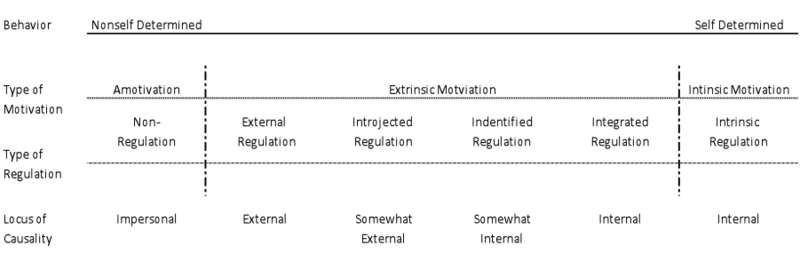
\includegraphics[width=0.8\textwidth]{Figures/oit.png}
    \rule{35em}{0.5pt}
  \caption{Organismic integration theory~\citep{ryan2000intrinsic}.}
  \label{figure:oit}
\end{figure}

SDT has been used to understand motivation for various activities or behaviours such as gaming~\citep{ryan2006:motivationalpull}, physical activity~\citep{power2011:obesity}, tobacco cessation~\citep{williams2006:testing} and energy saving~\citep{webb2013:self}. This study brings the motivational pull of gamification under the lens of SDT in order to understand how gamification can be used effectively in encouraging intermediaries to assist their respective beneficiaries in the utilization of personal health informatics. In the next section, the discussion of SDT is expanded through the lens of gamification.
\section{Self-Determination Theory Support in Gamification}
In order to understand why gamification may be important in intrinsic motivation, one has to understand the motivational triggers behind games.~\cite{knaving2013designing} framed the concept of games in terms of play and fun, where they conceptualized the terms as follows: (1) \emph{fun} is a rewarding and developmentally appropriate process necessary for survival, as it imparts humans with skills, knowledge and social cohesiveness; (2) \emph{play} is a voluntary engagement in an activity in order to have fun and feel pleasure; and (3) \emph{games} is formal play that is bound by rules. 

Games have defined goals and immediate feedback on progress towards those goals, and these are important mediators of optimal experience in play~\citep{knaving2013designing}.~One online survey~\citep{vella2013positively} with N=429 found that social play, relatedness during game play and flow (connection between goal setting and feedback) were some of the factors positively associated with players' psychological well-being.~\cite{ryan2006:motivationalpull} used self-determination theory to study motivational triggers in video games, where it was found that when aforementioned basic psychological needs were met, predicted the increase in enjoyment and the possibility of continuing to play the game in future. The importance of providing support for the three basic psychological needs has been emphasized  by situating the needs as part of motivational affordances to use ICTs with the objective of fostering motivation to use ICT systems~\citep{zhang2008motivational}. 

\cite{nakajima2013designing} argue that we should design systems to mimic the techniques used in games, to build emotionally engaging persuasive systems. The motivational aspects of gaming have steered researchers to explore their usage beyond the gaming context, and this has resulted in the advent of phenomena such as serious games and gamification. ~\cite{deterding2011game} considers gamification to involve borrowing ideas for motivating game design elements/patterns and applying them in a context outside the gaming environment. Gamification has a tendency to evoke intrinsic motivational experiences in users through gameful affordances~\citep{hamari2014persuasive}. Gamification is used outside the game context to increase interest in uninteresting but instrumental activities (e.g. physical activity and crowd-sourcing tasks such as image annotation). A systematic review on peer-reviewed studies found that the use of gamification was likely to have positive effects that are highly dependent on both the users of a gamified system and the context where a gamified system is used~\citep{hamari2014does}. Extrinsic integrated games have a practical advantage of having patterns that may scale well to different domains, while for intrinsically integrated games scalability may be a problem, and in practice it is much harder to design an intrinsically integrated game for each domain~\citep{preist2015use}.

\cite{hamari2014does} listed the most popular extrinsic motivators in gamification as ``\emph{points, leaderboards, story theme, badges, levels, goals, feedback, virtual rewards, progress and challenges}''. There are different schools of thought on whether gamification itself is a game or not. Most debates are centred around what a typical game entails (e.g. presence of rules, meta-games, immersion and voluntarism in their adoption)~\citep{seaborn2015:gamification}. According to~\cite{deterding2011game}, users of gamification can socially construct the meaning for what they consider gamification to be: they can perceive it as a game or, as some  other form of engagement depending on their context. The paper further argues that gamification is a gameful experience where an end user undergoes through an ``experiential flicker'' between different modes of engagement: gameful experience, playful experience or instrumental experience. This means that users alternate between perceiving a gamified tool as a game, and a state where a gamified system is perceived as instrumental for achieving a certain objective not related to game play. For instance, while users use a specific tool to achieve something, there is a possibility of the same people experiencing enjoyment from gameful or playful experiences.~\cite{seaborn2015:gamification} argued that the goal of gamified systems is different from games; therefore, it should rather be considered an act of integrating user experience with an activity outside the game context.~\cite{knaving2013designing} emphasized that while using gamification, the main activity being promoted should remain salient without being overshadowed by gamification; they recommended that designers should strike a balance between the preservation of an activity being promoted through gamification, and designing for playfulness. The goal of gamification should be to impart knowledge about the main activity being promoted, hence a design strategy should support both play and internalization.

\cite{sailer2013:psychological} provided examples of how game design elements can be mapped to the needs of competence, relatedness and autonomy; for instance, badges can be used to foster a sense of competence, while a leaderboard can be used to foster a sense of relatedness, as members of different teams are able to participate in competition with each other. A study by~\cite{hamari2013social} found the success of gamification to be dependent on social factors such as social influence, recognition, reciprocal benefit and network exposure, so in a gamified intervention, it is important to have a group of users that are committed to what a gamified system promotes.

\cite{mekler2013points} conducted a study to evaluate whether gamification harms intrinsic motivation. Gamification was added to crowd image annotation tasks. In that study it was found that gamification can increase engagement, but intrinsic motivation didn't change and was no different to the control group. Depending on how a gamified system has been designed, it can either foster or hinder the internalization of regulation that is externally rewarded. One way to foster intrinsic motivation is to ensure that gamification provides an optimal internalization (identified or integrated regulation).

There are some suggestions of how one could use gamification to promote motivation towards optimal internalization. An example is to make gamification meaningful. An experiment that examined facilitating contextual factors that can foster internalizing the regulation of a behaviour, found that factors such as framing the task with a meaning (providing a meaningful rationale), being sympathetic towards the behaver's  feelings and conveying choice fostered integrated regulation~\citep{deci1994facilitating}.~\cite{nicholson2012user} presented a framework for meaningful gamification that put the user at the centre. The framework was inspired by organismic integration theory explained above, situational relevance and situated motivational affordance, universal design for learning, and player-generated content. An example of meaningful gamification is where users are convinced that what they are doing is not just for the sake of playing a game but rather for contributing to a good cause. For instance,~\cite{mekler2013points} used points and a leaderboard to encourage participants in image annotation tasks and found that even though gamification did not harm intrinsic motivation, it negatively affected the quality of image annotation as participants were focusing on completing more tasks in order to advance in gamification. The same experiment was repeated, except this time it included gamification with meaningful framing, where participants were informed how each tagging was instrumental in improving computerized affective image categorization and, as a result, contributing towards an advancement in science. This was an appealing cause to the participants, hence it resulted in better quality tags being produced by participants in the meaningful framing condition~\citep{mekler2013disassembling} compared to participants in gamification without meaningful framing. In the context of this research, I hypothesized that pairing an intermediary and beneficiary that have a good social relationship would help intermediaries view the activity of assisting their beneficiaries as a good cause as they would be helping people they care about; hence it was anticipated that this framing would cause the collaborative gamified system to be perceived as meaningful.

The next section presents utilization of games and gamification in health interventions and what is lacking in literature as far as those interventions are concerned, with regard to supporting the utilization of personal health informatics through intermediary users.

\section{Utilization of Games in Personal Health Interventions}
Following the success of games as platforms for entertainment purposes, there is a paradigm shift towards using such platforms to influence positive changes in health behaviours~\citep{king2013gamification}. There is an increasing interest in using games to engage people with personalized health interventions~\citep{mccallum2012gamification}. Traditional design of games encourages people to remain sedentary; however, the new direction of research brings body movements into the game play. Games for health include but are not limited to exergames, games with purpose (serious games) and gamification. These classes of games are discussed in the next subsections. 
\subsection{Exergames}
Exergames combine exertion (body movements that are beyond sedentary activities) and video games. Exergames may include strength training, balance and flexibility activities~\citep{oh2010defining}. Exergames increase the amount of energy expended by the body~\citep{graves2010physiological}. Examples of exergames include  dance video games, e.g. Dance Dance Revolution~\citep{lieberman2006dance}, or games such as Nintendo Wii Fit~\citep{gobel2010serious}. There are also exergames that have been designed to be used for outdoor activities.~For instance, Zombies Run! is an outdoor exergame that gives users the experience of immersion while jogging; this immersion is achieved through interesting narratives about zombies who appear to chase the runner at specific points of the story. This makes the runner respond by running much faster in order to avoid being caught by zombies~\citep{southerton2013zombies}. With an exergame, one can become more active, but its use should never be confused with exercise~\citep{oh2010defining}. According to~\cite{caspersen1985physical} cited by~\cite{oh2010defining}, ``\emph{Exercise is doing a physical activity intentionally to improve or maintain physical fitness with a planned, repetitive, and structured format}''. Playing an exergame entails exertion, but it remains a physical activity which may be for entertainment purposes, unless that activity is performed according to the definition of exercise~\citep{oh2010defining}. However, playing an exergame is better than playing a sedentary video game, as the former promotes physical activity which is important in increasing energy expenditure. This form of energy expenditure, which doesn't fit into a category of exercise, is known as \emph{NEAT} -- non-exercise activity thermogenesis. NEAT activities such as walking, taking stairs or exergaming (playing exergames) have been found to expend a significant amount of energy~\citep{fujiki2008neat}. Exergames have application in health settings as they can be used to support rehabilitation~\citep{mccallum2012gamification}. In one study, the use of exergames was compared with traditional methods of physiotherapy. It was found that exergames performed significantly higher in scores of autonomy, presence, and in functional reach tests~\citep{smeddinck2015exergames}. The exergames consisted of a collection of different games that allowed players to perform bodily movements such as raising their hands in order to pick apples from a garden, and placing them in a basket near the ground. This required players to bend their bodies. Users had sensors attached to their bodies, and their bodily movements could make virtual avatars perform certain tasks on a screen. This is a common way of controlling characters in many games, including the sedentary ones which entail the use of physical input devices such as game consoles, keyboards, or other sensory mechanisms to support players' embodiment of virtual characters or avatars~\citep{berkovsky2012physical}. So the approaches used to control avatars in games for health purposes are somehow similar to the ones used in conventional electronic games. 

The benefits of exergames are not limited to younger populations.~\cite{brox2011exergames} revealed that exergames could also be accepted by elderly populations. In one study by~\cite{brauner2013increase}, an exergame was developed where players had to pick fruit and vegetables from a virtual garden using an avatar that represented them on screen. Interaction with an avatar happened through a Microsoft kinetic sensor for detecting body movements and gestures. The game was found to be enjoyable by the elderly participants. However, features to support personalization and persistent storage of players' information were not present in that game; in such a scenario players cannot resume from a previous state of the game play. In addition, the only interaction was through bodily movements. There was no complex navigation (in many other systems, several layers of user interfaces are required in order to reach the main feature). This implies that navigation to the main gaming interface was less sophisticated, and may have required less cognitive effort on the part of users in comparison to typical gamified personal health informatics systems, which may require users to navigate across several layers of user interfaces before firing an action. It is possible for a user interface of a personalized system to appear sophisticated to users who are not conversant in technology. Older adults are an example of a demographic group that might face barriers in navigating user interfaces.~\cite{chen2016social} evaluated an app that implemented social incentives to encourage obese and diabetic patients to exercise, and it was found that technical literacy is a challenge for older patients. A review on popular personal apps has revealed that many do not accommodate the needs of older adults~\citep{silva2014:smartphones}; hence this study emphasizes that one can leverage existing usage through intermediaries for such population groups, as this mode of interaction is already prevalent in many low-income communities of developing countries. Such an interaction may be possible in collectivist societies~\citep{parikh2006}. The idea of collectivism in the utilization of personal health systems has been emphasized in the dimension of having a community of users that collaborate in the management of health information~\citep{colineau2011motivating,grimes2009toward}, or different users of personal systems sharing health information among one another across social media~\citep{ploderer2014social}, but not in the respect of having one user supporting another user in their information needs through a single collaborative user interface. For instance, literature reports on exergames and systems that support competition in health self-reflection, where such systems involve  parents and children working together~\citep{grimes2009toward,saksono2015spaceship}, but their study was not done in the context of one user supporting the other user to navigate through user interfaces.
\subsection{Serious Games in Health}
Serious games have been defined as games that are designed to achieve a specific goal of change in the player's knowledge, attitude, physical ability, cognitive ability, etc. Serious games are sometimes referred to as games with purpose: their intention is to provide experience and emotion with the goal of conveying a meaning~\citep{marsh2011serious}. Areas in which serious games can be utilized for personal health include preventive (exergames), therapeutic (rehabitainment), assessment (self-ranking), educational (medical information) and informatics (personal health records)~\citep{mccallum2012gamification}. As serious games add user experience to an outside activity (probably an uninteresting one), there is an overlap of goals between serious games and gamification. The two terms are sometimes used synonymously (interchangeably).

There has been a rapid increase in the number of gamification-related studies in the persuasive technology field~\citep{hamari2014persuasive}. One prevalent utilization of gamification is to promote physical activity, with the aim of promoting NEAT physical activities as they are more omnipresent in people's daily lives compared with volitional sporting activities, which are mostly constrained by location and time~\citep{fujiki2008neat}. The urgent need to promote non-exercise physical activity is a result of the prevalence of electronic screens such as televisions and computers, which has increased the tendency of people to be more sedentary~\citep{berkovsky2010physical}. One study~\citep{levine2006non} cited in~\cite{fujiki2008neat} found that obese participants were spending more time (164 minutes longer on average) seated  compared with lean participants. There is a need for pervasive and ubiquitous computing to support people to become more aware of their lifestyle in order to foster an increase in non-exercise energy expenditure and reduce the quantity of calories consumed. This section provides examples of systems that use games/gamification in motivating particular healthy  behaviours through self-monitoring. These systems utilize various techniques such as points, avatars, virtual pets and leaderboards that have already been discussed above. 

\cite{lin2006:fish} developed and evaluated the Fish'n'Steps system, a computer game in which growth of a fish in a tank, together with its emotional state, is directly linked to footsteps of a player that have accumulated throughout the day. The application was evaluated with a total of 19 participants in a 14-week study. The findings indicated that the game catalysed the promotion of exercise and improvement of players’ attitudes towards physical activity. The authors observed that players' enthusiasm in playing the game had declined towards the end of the second week of using the application, mainly due to players already becoming accustomed to the new routines of a healthier lifestyle. 
  
\emph{{NEAT-o-Games}}~\citep{fujiki2008neat}, a comprehensive collection of PDA-based games, allows players to accumulate physical activity points which they can use in a virtual race. In order for an individual to accumulate points from physical activity, there is a wireless transmission of physical activity from a wearable accelerometer to a PDA, resulting in the player's animated avatar moving forward in a virtual race. Each player's position in the race corresponds to their current physical activity points. A player with the highest physical activity points leads the race. A player can also decide to use physical activity points to get hints while playing a puzzle-solving game called Sudoku. Using points in Sudoku means a player drops behind in a race game, and more steps (physical activity points) are required. In a pilot experiment with 8 participants, the authors indicated that participants increased their physical activity while enjoying playing the collection of games. 

The~\emph{Flowie} system, designed for home settings, is a virtual coach used to motivate elderly individuals to increase their amount of walking. The system consists of a frame casing with a touchscreen display that shows a flower whose vitality corresponds to the amount of physical activity captured by using context-aware sensors~\citep{albaina2009flowie}. A concept similar to the Flowie system is that of UbiFit Garden, which generates a garden with flowers of different types that discern different types of activity such as cardio, walking and housework~\citep{klasnja2009:using}. The authors showed the usefulness of living metaphors such as garden flowers in communicating information about physical activity level, as it makes an interaction experience to be more enjoyable and engaging to end users.

\emph{StepCity}, a strategy-based game~\citep{walsh2014stepcity}, is controlled through accumulated footsteps. In a StepCity game, players connect their Fitbit accounts\footnote{https://www.fitbit.com/} to the game. Players' accumulated steps can be used as currency in the game to buy buildings to place in players' respective cities that produce gold and increase population. Buildings have side effects, as cheaper buildings produce more crime while more expensive ones produce none. Players can move through various stages of civilization, and a leaderboard is used to rank cities by the amount of gold, crime and population. In evaluation there were three experimental conditions: the control group (only Fitbit), the social interaction experience (app supporting interaction between participants), and the StepCity game. The results of evaluating the game with 50 users showed that newer Fitbit users (n=41) had more steps than the amount accumulated during the control period (at the beginning, before starting to use the game) without statistical significance; however, the overall results were inconclusive.  

There are also other studies that used gamification to motivate adolescents or teenagers in behaviours such as frequent monitoring of blood glucose or physical activity~\citep{arteaga2010:persuasive,cafazzo2012:bant}. Apart from interventions that target promotion of physical activity, there are game-based apps designed to encourage healthy eating. An example of such an app is a mobile game called \emph{It's Time to Eat}, which was specifically designed to motivate children to practise healthy eating habits through taking care of their virtual pets~\citep{pollak2010s}. In the game, players select a pet from a range of options such as a worm, dinosaur, dog and tree. Then players are required to take care of their selected pets. The first step is for players to choose names for their pets. The process of selecting a pet and naming it is meant to give a player a sense of control or autonomy. Caring for a pet entails a player feeding it by uploading a photo of their breakfast, and then a nutritionist gives it a certain score. Based on the total score, a virtual pet responds with an emotional state. A healthy breakfast results in a pet becoming happy, while an unhealthy meal makes the pet sad. The finding from this study indicated that kids who had played the game had an inclination towards eating a healthy breakfast more frequently than those who didn't play the game~\citep{pollak2010s}. Another diet-based game is called \emph{LunchTime}~\citep{orji2013lunchtime}, aimed at educating people to make healthy choices while eating away from home. This application utilizes the following persuasive strategies: goal setting, feedback, social influence and rewarding mechanisms. In~\cite{orji2013lunchtime}'s study, the game was played by a group of friends visiting a restaurant as customers. The game awarded points to players according to how healthy the choices of their meals were. A 10-day evaluation  of LunchTime, with 6 participants (three males and three females) aged between 19 and 40 years of age, indicated that the application facilitated learning and reflection. In addition to that, attitudes towards healthy eating showed improvement at the endline in comparison to the baseline. 

An example  of a different use of games is the supporting of heart-rate monitoring, for instance in the case of \emph{Live Pulse Games}~\citep{han2014designing,han2015balancing}. Live Pulse Games is a collection of games that employ a novel technique to measure users' heart rate in real time, by having them play casual games on their mobile phones. In order to gain some in-game control, the player has do some covering of the camera lens with their fingertips during the game play. For instance, one game within Live Pulse Games is called \emph{City Defender}. In this game, an end user has to load the anti-aircraft artillery through lens-covering actions. The heart rate is computed by detecting changes  in  blood transparency in the user's fingertips.
 
Another approach to gamification does not involve adding user experience to a targeted health behaviour; instead, a motivating sedentary game is interlaced with the targeted health behaviour. This approach is based on Premack's principle~\citep{premack1959toward}, which suggests using an event with high probability, such as playing a computer game, to motivate an activity with low probability, such as doing physical activity. An example of a game that utilizes such an approach is one called \emph{PLAY MATE}~\citep{berkovsky2010physical,berkovsky2012physical}. This game takes advantage of motivation factors in video games by introducing a burst of physical activity during a session of  sedentary game play. \emph{PLAY MATE} is an alteration of an open-source computer-based game called \emph{Neverball}, which gives a player a limited amount of time to collect coins~\citep{berkovsky2012physical}. In the design of PLAY MATE, incentives of extra time are given to a player for each jump that is performed in the middle of a session of sedentary game play~\citep{berkovsky2012physical}. Jumps are detected through a sensory device (built with an accelerometer and gyroscope) worn on the waist. The preliminary evaluation of this system indicated that skilled players had a tendency to perform fewer jumps compared with less skilled players; hence the game was modified to include an adaptive algorithm by which the level of difficult was personalized according to a player's completion time of previous levels.

A similar idea implicitly utilizes Premack's principle~\citep{premack1959toward} in education settings.~\cite{preist2015use} looked at enjoyable game playing combined with revising for an examination.Their approach used the F2P (free-to-play) game business model, where users are presented with a fully functioning game that is freely available but has an option to do micro-payments in order to either speed up game play (e.g. speed up resource gathering used to advance technology for combat in a strategy game) or provide access to virtual goods. This study used a game strategy similar to Clash of the Clans to motivate 15- to 16-year-old children to revise in preparation for a mathematics examination. The option of micro-payment was substituted with virtual currency earned through taking revision tests at any time within the game play. An experiment was performed to discern the effectiveness of the educational game in comparison to two groups which were control, and the quiz generator software. The findings from that study indicated a statistically significant improvement in performance (based on pre-post scores of the test) on learners that were assigned to the game group~\citep{preist2015use}. Even though the experiment was conducted in the learning context, one could adapt the same concept to the context of promotion of health behaviours.

Most of the health-based interventions reported in the literature are carried out in contexts that are not constrained by resources, with the exception of a few, such as the one that developed an exergame for families in low socio economic areas~\citep{saksono2015spaceship}, or another study that used user-centred approaches in the development of mobile game-based applications for the promotion of physical activity in youths with low socioeconomic status~\citep{blackman2016developing}. Literature on utilization of serious games in developing world contexts is scarce and existing studies tend to focus on education~\citep{kam2008designing,botha2015icts}.

In this research, the focus was on health interventions within the context of low-resource settings of a developing country, which may not be the same as a context of low socioeconomic status in developed countries. One of the drawbacks of those gamified personalized interventions is that they tend to be designed for direct/primary users of technology, as only direct beneficiaries are considered; leaving out indirect beneficiaries (those that depend on intermediary users for facilitating access to user interfaces). In most of these interventions, the person (an adult or young person) who is a targeted beneficiary of the information on the app is expected to be an actual manipulator of the user interfaces of such a system. Most of the motivational incentives provided by such systems target direct users, who in most cases are younger and technologically literate. None of the aforementioned studies have explored the utilization of gamification where one user facilitates an interaction process while an actual beneficiary remains an observer or indirect/secondary user. Thus this study aimed to explore how one could implement motivational incentives (affordances) to target a pair that consists of an intermediary user and a beneficiary user. Literature on intermediated technology use has shown that young people within a community may fit well as intermediary users. In addition, young people have more of an inclination to play computer games than the elderly~\citep{brauner2013increase}. There is an opportunity for leveraging the  motivation of young people through gamification to foster collaboration between adults and children, with the goal of children engaging adults who may be less conversant or less motivated to engage with gamified personal health informatics. 

\begin{flushright}
\end{flushright}

% Chapter 1

\chapter{Study Context} % Main chapter title

\label{contextchapter} % For referencing the chapter elsewhere, use \ref{Chapter1} 

\lhead{Chapter 1. \emph{Study Context}} % This is for the header on each page - perhaps a shortened title

%----------------------------------------------------------------------------------------
\section{Obesity}
This section describes obesity from a clinical point of view to show the link between obesity and lifestyle. Obesity is the  result of a positive imbalance between what is consumed and what is expended by the body, where excess energy is stored in fat cells~\citep{steyn2006chronic}. This positive imbalance is due to two factors: (1) overeating, especially of an energy-dense diet (food that is high in either fat or sugar), and (2) a sedentary lifestyle. Results of well-conducted randomized control trials have concluded that these two factors increase the risk of obesity~\citep{swinburn2004diet}.

An energy-dense diet is one that is high in simple carbohydrates, which may result in a sharp elevation  of postprandial insulin levels that could lead to increased triglyceride storage in the adipose tissue depots. After a spike in the insulin level, the body senses that it has consumed all this energy but it doesn't need it all; hence it stores it in fat cells. If many cycles of storage occur, there will be an increase in fat depots, and if a person expends less energy than what is taken in, then the fat will remain in those depots. As insulin spikes happen, it is likely for a person to feel hungry soon after eating. This is due to an immediate conversion of all the sugar into energy, which the body then converts into fat upon realizing it exceeds the current required energy. The fat is then stored in depots; hence there is no sugar left in the bloodstream, and as a result the person may be tempted to keep on eating to compensate for depletion of glucose~\citep{bouchard1993exercise}. This poses a risk of going into many cycles of eating and being predisposed to binge-eating disorder~\citep{collins2009behavioral}. Individuals with binge-eating disorders lose self-control of their eating patterns. Therefore, as the person becomes obese, they are likely to lose control of their eating pattern and this may worsen their current situation of obesity. 

Most of the time, clinical diagnosis of obesity relies on measuring body mass index (BMI), which is obtained by dividing the person’s weight in kilograms ($kg$) by their height in metres squared ($m^2$). In some populations, a person is considered obese if their BMI is above 30 $kg/m^2$~\citep{steyn2006chronic} while in other populations the cut-off point may be different. There is controversy about using BMI alone, as some people can weigh more but may not necessarily be obese (having extra fat), because the extra weight may be due to having extra muscle, bone or water; hence in addition to BMI, it is recommended to also measure waist circumference to clinically diagnose obesity~\citep{janssen2004waist}. 

People with a BMI over 30 $kg/m^2$ are predisposed to the risk of co-morbidities related to obesity~\citep{de2000clinical}. Therefore, lifestyle modification is crucial in dealing with the obesity pandemic. The next section provides more background on the relevance of the problem within a South African context.
\section{Context Description}
This research conducted its studies with participants from low socioeconomic neighbourhoods of Cape Town, South Africa. There were four study sites, of which one was a diabetic and endocrinology clinic which is frequented by patients from low socioeconomic areas, while the remaining sites were three low socioeconomic townships in South Africa. 

The rationale for  deciding to work with participants from low socioeconomic neighbourhoods is supported by literature. A review by~\cite{dinsa2012obesity} suggests that in countries with medium human development index, of which South Africa is one, groups of low socioeconomic status are also affected by obesity, and the trend shows that women of low socioeconomic status are mostly affected compared with women of high socioeconomic status. Some barriers to adopting a healthy lifestyle that are present in low socioeconomic communities in the west also appear to occur in low socioeconomic urban communities in Cape Town. Studies that have been conducted in developed countries reveal that, in low socioeconomic areas, some environmental factors may influence behaviour patterns that predispose individuals to obesity. The environment may play a role in both promoting the intake of unhealthy food and in discouraging physical activity. Some of these factors could be lack of access to recreational facilities, a poorly designed built environment which lacks roads for pedestrians, or a lack of public transport that then promotes the use of private transport. The environments in which people live are complex and their individual and combined elements have a marked effect on behaviour and dietary intake~\citep{swinburn2004diet}. Food choices can be largely influenced by cultural issues and other factors such as price, portion size, taste, variety and accessibility of foods~\citep{ali2009factors}. The environment may also promote obesity by increasing the likelihood of consuming big portions of meals that are considered high in fat~\citep{hill1998environmental}. These contextual factors that may put individuals at risk of becoming overweight or clinically obese were also present in the context of participants of this research. Many low-income neighbourhoods in Cape Town are not safe, and this prevents people from doing simple physical activity such as walking. In addition, the meal outlets in townships sell food that is high in calories. In the contextual enquiry (Chapter \ref{contextualenqchapter}), the majority of the diabetic and obese participants claimed that healthy food in supermarkets is expensive, and they have to eat what the rest of the family eats because they cannot afford to prepare two separate meals. The preliminary study (Chapter \ref{contextualenqchapter}) observed that the notion of healthy food is not quite understood, therefore the application that was tested in this context helped participants to understand that you can still live a healthy life by utilizing whatever resources you have. The aim of this research was to explore how to design in order to support motivation in intermediated use of personal health informatics in the context of South African low-income townships. 

The problem of obesity in South Africa is quite alarming. Statistics show that almost 60\% of South Africans are overweight~\citep{ng:global}. Urbanization and emigration of people from upcountry to cities  have been suggested as possible reasons for the adoption of unhealthy behaviours, as the city lifestyle encourages people to be more sedentary and increase their consumption of caloric-dense food~\citep{ali2009factors}. The populations that live in low socioeconomic areas face numerous challenges. Most apartheid policies regarding health did not focus on these populations, and some of the current health and economical concerns are a result of amplifications of apartheid social clusters \citep{benatar2013challenges}. This is why it is crucial to focus on low socioeconomic areas in order to understand technology design constraints for these marginalized populations. In addition to the health concerns, we have already discussed how sharing of technology and the presence of indirect use could hamper utilization of technology for health interventions in low socioeconomic areas of developing countries.   
\begin{flushright}
\end{flushright}

% Chapter 1

\chapter{Contextual Enquiry} % Main chapter title

\label{contextualenqchapter} % For referencing the chapter elsewhere, use \ref{Chapter1} 

\lhead{Chapter \ref{contextualenqchapter}. \emph{Contextual Enquiry}} % This is for the header on each page - perhaps a shortened title

%----------------------------------------------------------------------------------------
\section{Study Description}
The purpose of this contextual enquiry was to elicit preliminary requirements to inform the design of an early prototype of a personal informatics application to be utilized through intermediaries. The study generated these requirements based on insights garnered from exploration of (1) issues related  to technology utilization; and (2) barriers to adoption of healthy behaviours. I was able to generate these insights from the data we collected in hospital settings with patients who qualify as prospective beneficiaries of such technology in future. The main goal of conducting a contextual enquiry was to gather contextual factors related to utilization of cellphone technology among obese adult patients. I obtained the ethical approval for this study from the Human Research Ethics Committee of the Faculty of Health Sciences at the University of Cape Town (see Appendix A).

I worked together with one research assistant in order to carry out this contextual enquiry. Between March 2013 and May 2013, we recruited a convenient sample of diabetic patients at the diabetes and endocrinology clinic at Groote Schuur Hospital in Cape Town. This is an outpatient clinic which runs on Thursdays and Fridays.

We opportunistically approached participants as they waited to see their doctors. We conducted interviews in one of the vacant consultation rooms, which guaranteed confidentiality and privacy of the participants. The main topics in these semi-structured interviews focused on participants' general utilization of mobile phones and specific usage for health, whether they sought help from intermediaries and, if so, who their preferred intermediaries were. In addition, we explored their current barriers to both exercise  and the adoption of a healthy diet.

We obtained our data from a total of 30 participants, 20 of whom were female. The majority of the participants had primary- and secondary-level education as shown in Figure \ref{figure:education_level}. The distribution of participants by ethnicity is shown in Table \ref{table:ethnicity} and all were from previously disadvantaged races during the apartheid era in South Africa. Most of the participants were low-income earners (Figure \ref{figure:income_distr}); this income data was for individuals and not households. Twenty-three percent had no income and depended on their family members to sustain them. In this group of people with no  sustainable income, only one person was 21 years of age, the remainder being above 40 years of age.
\begin{figure}[htbp]
  \centering
    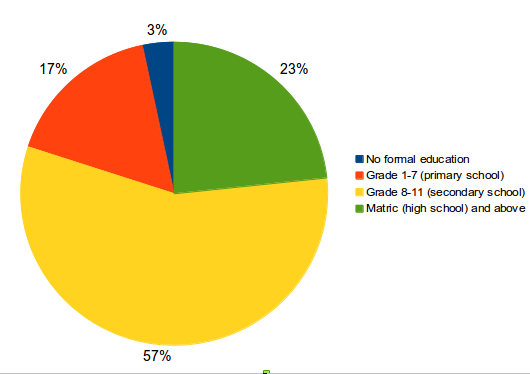
\includegraphics[width=0.6\textwidth]{Figures/education_level.png}
    \rule{35em}{0.5pt}
  \caption{Participants' education level.}
  \label{figure:education_level}
\end{figure}

\begin{table}[h!]
  \begin{center}
    \caption{Ethnicity of contextual enquiry's participants.}
    \label{table:ethnicity}
	\begin{tabular}{|p{3cm}|p{4cm}|p{2cm}|}
		\hline
		\textbf{Ethnicity}&\textbf{No. of Participants}&\textbf{Percentage}\\
		\hline
		 Black African&8 &26.67\% \\
		\hline
		 Coloured&22& 73.33\%\\
	\hline
	\end{tabular}
  \end{center}
\end{table}

\begin{figure}[htbp]
  \centering
    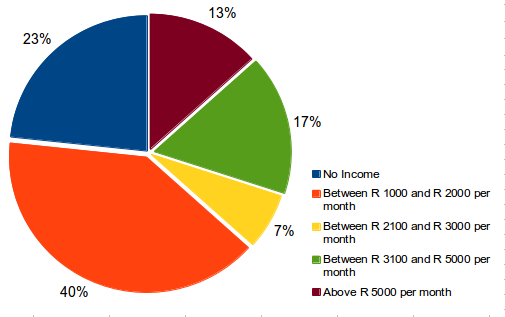
\includegraphics[width=0.6\textwidth]{Figures/income_distr.png}
    \rule{35em}{0.5pt}
  \caption{Participants' income distribution.}
  \label{figure:income_distr}
\end{figure}

Demographic information indicated the average BMI of the participants was reported to be 33.36 $kg/m^2$ (standard deviation of 5.74 $kg/m^2$); hence the majority of the participants were overweight, with fewer appearing to be clinically obese. The average age was 53.13 years old (standard deviation of 11.77 years old).  Almost 86\% (26) were above 40 years of age. This means we were dealing with old participants who were generally inexperienced or less conversant with technology.

\section{Data Collection Methods and Analysis}
We used a semi-structured questionnaire (Appendix E) to interview participants, each of whom was interviewed for 20 to 30 minutes. The questionnaire consisted of four groups of questions: demographics; cellphone ownership and utilization; access to information and pedometers; and barriers to diet and physical activity.~Based on their answers, we asked follow-up questions to seek clarifications on some of their responses.~We recorded responses for each participant on paper.

I used both descriptive statistics and qualitative approaches to analyse the information obtained from participants’ responses. Although our objective was to interview overweight and obese patients only, we included those who appeared to be thin but were diabetic. Since diabetes is a lifestyle-related disease, we felt that it would be interesting to also understand utilization of cellphones, and access to information even by individuals who appear not to be overweight but who may have some input in various issues related to technology utilization, and  barriers to adoption of healthy behaviours. All the names in the presentation of findings are pseudonyms to protect the privacy of participants. 
\section{Findings}
\subsection{Utilization of Cellphones}
Twenty-nine out of the 30 participants owned cellphones. The services most used were SMS and voice, with at least 80\% of the participants using both. At least 60\% of the phones owned by participants were smartphones (Figure \ref{figure:cell_ownership}), but utilization of functionality/services that are supported in smartphones was lower relative to voice and SMS (Figure \ref{figure:cell_utilization}). Utilization of services supported on smartphones only decreased with age. Utilization of WhatsApp was higher compared with other services that are specific to smartphones; participants were influenced to use WhatsApp by family members and friends who were already using WhatsApp. These influencers suggested that WhatsApp was cheaper than SMS. For instance, one 47-year-old male participant heard that WhatsApp was cheap for communication, and his son helped him load it on his phone. Therefore, in this context, social influence played a role in the adoption of some services that are supported only in smartphones. There is a positive correlation between social influence and adoption of high-tech innovations \citep{vannoy2010social}.  

\begin{figure}[htbp]
  \centering
    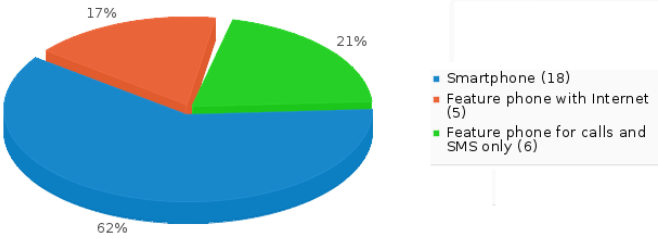
\includegraphics[width=0.5\textwidth]{Figures/cell_ownership.png}
    \rule{35em}{0.5pt}
  \caption{Participants' phone types.}
  \label{figure:cell_ownership}
\end{figure}

\begin{figure}[htbp]
  \centering
    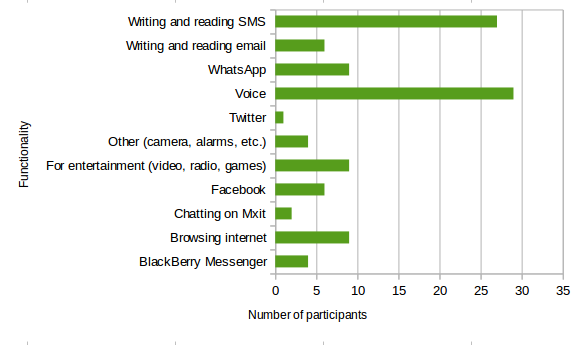
\includegraphics[width=0.5\textwidth]{Figures/cell_utilization.png}
    \rule{35em}{0.5pt}
  \caption{Utilization of cellphone functionality/services by participants.}
  \label{figure:cell_utilization}
\end{figure}
\subsection{Help-Seeking in Utilization of Cellphones}
There were several scenarios of informal help-seeking in utilization of cellphones as highlighted in Table \ref{table:intermediated}.

\begin{table}[h!]
  \begin{center}
    \caption{Scenarios of intermediated interactions.}
    \label{table:intermediated}
	\begin{tabular}{|p{0.5cm}|p{13cm}|}
		\hline
		 \textbf{No.}&\textbf{Scenario}\\
		\hline
		 1& Her \emph{daughter} helps her read SMSes by her, but she can do it on her own when the daughter is not around. \\
		\hline
		2&He doesn’t know how to reply to an SMS, so his \emph{grandson} always helps him with that.\\
	\hline
	  3&Her \emph{children} or  \emph{work colleagues} help her read SMSes written in English that are received through her feature phone. She also mentioned that her two children were more skilled than her in operating a cellphone one of them had a BlackBerry smartphone.\\
	  \hline
	  4&He can take photos using his mobile phone’s camera but he doesn't know how to save those photos on a memory card. His \emph{son} helps him with that once in a while. His son also helped him load WhatsApp on the phone.\\
	  \hline
	  5&Her \emph{children} have taught her how to use WhatsApp, take videos, etc. Now she is learning how to record sound and set alarm (reminders) on the phone for insulin and medication.\\
	 \hline
	 6&The \emph{son} helps her interact with the USSD service to check loyalty points on MTN. MTN is a mobile communication service provider operating in many African countries.\\
	 \hline
	7&She was taught by  her \emph{son} how to access a phonebook when composing SMSes using her new phone.\\
	\hline
	8&She receives assistance from her \emph{helper} when she wants to send messages to her children.\\
	\hline
	9&She was once helped to set up her new phone at a cellphone shop. She was also taught how to operate BBM by her \emph{grandson}.\\
	\hline
	10& He was once taught how to operate WhatsApp by his \emph{niece}.\\
	\hline
	11&Her \emph{son} and \emph{grandson} once helped to configure WhatsApp and Facebook on her phone. They have also taught her how to use those two web services. In addition, she also asks the son to search for certain health information on the Internet, and once the search is done the son passes the phone to her to view that information. This happens once a month.\\
	\hline
	12& Her \emph{son} and \emph{grandson} teach her how to use various functionalities like games, etc., but she is not that keen on operating those functionalities. She also admitted that her son and grandson are very interested in their mobile phones and they spend a lot of time playing on their phones, which is something she doesn't understand.\\
	\hline
	13& This participant does not own a cellphone. She has no formal education and is unfamiliar with how to operate a cellphone. Her son receives SMSes directed to her and reads them aloud for her or translates an SMS to verbal communication. Also, the son receives phone calls and hands over the phone to her when the person on the other end of the line wants to speak to her.\\
	\hline
	\end{tabular}
  \end{center}
\end{table}

The majority of the participants had solicited  informal help from other people before to configure services/apps on their phones (e.g. WhatsApp, Facebook); in the habituation of skills required for utilization of various functionalities (e.g. a phonebook of a new or unfamiliar cellphone, WhatsApp); and to interact with certain features such as SMS and Internet browsers.

There was a variation in the degree of help-seeking that was determined by how often participants wanted to execute unfamiliar tasks. Tasks such as configuration of services and apps or teaching of individuals were rare occurrences, as they only happened when participants encountered a new application or device and did not know how to make it functional. For frequent used applications, where participants were not able to utilize them entirely on their own, they sought for assistance by intermediaries more often. The next section highlights the characteristics of intermediaries that were mostly picked by participants.
\subsection{Selection of Help-Givers}
Participants chose trusted individuals to act as their help-givers, typically their children and grandchildren or, less often, children of relatives, family friends, or someone at a cellphone shop. The most likely to be solicited to assist were family members. Help-givers were selected based on the merit of skills/competence; interpersonal trust based on a social relationship; and past experience of help-seekers with specific help-givers.
\subsubsection*{Interpersonal trust}
Interpersonal trust in this context means whether help-seekers feel comfortable seeking help from specific people or not. Privacy and the existing relationship between a help-seeker and help-giver were the first concerns when deciding who to ask for help. An additional factor was whether the help-seeker could trust a helper-giver to deliver when solicited for help and this was influenced by past attempts -- positive and negative -- at seeking help. These experiences shaped perceptions of some of the participants about seeking help with cellphone or any other technology. For instance, one  67-year-old female participant reported that her daughter helped her once but she had no patience. A male participant aged 47 mentioned that he would like assistance when using services such as MMS, but that young people do not have patience to help. Such negative experiences can prevent help-seekers asking certain help givers for assistance. This resonates with the finding by~\cite{kiesler:twi} that parents may be reluctant to seek informal help from their children after encountering negative experiences.
\subsubsection*{Help-givers' Competence}
In addition to interpersonal trust, deciding who to solicit for help was also influenced by the help-seekers' level of trust of the skills possessed by help-givers. Participants were confident that their children could use cellphones competently. Several participants thought their children had the technical know-how to use cellphones. For instance, one 31-year-old female participant mentioned that her five-year-old son knows how to navigate through her entire phone and use it more than she does. Another female participant, aged 56, explained how children are eager to teach her various things on a cellphone but she is not that keen to use cellphones like her son and grandson do. A 47-year-old male participant, mentioned that, within the family, young people are more skilled at using cellphones than old people.
Participants reported that their kids were borrowing their phones to do other tasks and this demonstrated that their kids had better skills with technology. Scenarios of sharing are presented in Table \ref{table:phone_sharing_contextual} below. 

\begin{table}[h!]
\begin{center}
    \caption{Scenarios of sharing of cellphones between participants and their children.}
    \label{table:phone_sharing_contextual}
	\begin{tabular}{|p{1cm}|p{12cm}|}
		\hline
		 \textbf{No.}&\textbf{Scenario}\\
	\hline
	1&``Zandile'', a 47-year-old female, mentioned that her 16-year-old son would borrow her phone to use Mxit. Zandile does not use anything else on the phone apart from calls and SMS. She also said that she is not much interested with technology. For example, she has Internet at work, but does not really use it.\\
	\hline
  2& ``Buyisiwe'', a 31-year-old female, narrated an experience about her five-year-old son who uses her smartphone to listen to music. But she has to lock it while he is listening, because on one occasion he deleted almost everything on the phone.\\
  \hline 
  3&``Celine'', a 48-years-old female, lends her phone to her daughter who uses it for normal Internet browsing and Facebook. Celine owns an advanced feature phone that is Internet-enabled, but she does not use Internet on the phone.\\
  \hline
	\end{tabular}
  \end{center}
\end{table}
In other scenarios, participants mentioned that their kids borrow their phones to search for information related to school assignments. These examples demonstrate the level of skills that potential help-givers can have. Trust in the skills possessed by help-givers has been found to be very important to individuals seeking help in the ICTD and HCI contexts.~\cite{ramirez2013infomediaries} suggests that empathy and technical skills of infomediaries influence the outcomes of the process of infomediation to users at public access venues. Another study that examined motivations for informal support in utilization of computers at home found skills of help-givers to be one of the factors that influence help-seekers to solicit help from specific people~\citep{poole:chh}. 
\subsection{Access to Health Information and Self-Monitoring Support}
We also collected data on how participants currently access information pertaining to health. In addition we collected data on how participants' currently self-monitor health. Informational support on which most of the participants rely is that provided through face-to-face meetings with doctors or dietitians during hospital visits. Normal hospital visits are scheduled every three or six months, but participants visit the hospital only two or three times a year. In addition to face-to-face information, patients normally receive paper sheets that provide guidance on how to eat healthily. These are usually received when patients attend the clinic for the first time after being diagnosed with diabetes. Most patients we interviewed were type 2 diabetics and overweight. Doctors and nurses encourage them to eat healthily and to exercise. 

The majority of the participants lacked informational support beyond hospital settings that could provide guidance for healthy eating  and exercising.~Very few participants had used cellphone services to query or receive information related to health. Only six participants had used the Internet to search for health information, while only one participant had used a cellphone app for health. Only two participants had used SMS, while only one had used voice to look for health information. Table \ref{table:health_information} shows some of the scenarios of were participants used ICTs in relation to learning about issues concerning their health.
\begin{table}[h!]
\begin{center}
    \caption{Participants’ usage of ICT to fulfil health information needs.}
    \label{table:health_information}
	\begin{tabular}{|p{1cm}|p{12cm}|}
		\hline
		 \textbf{No.}&\textbf{Scenario}\\
		 \hline
		 1&``Anitha'', a female participant aged 56, sends SMSes to her son while he is at his workplace. These are usually requests to check for certain  health information on the Internet, and the son then prints all the relevant material. She also follows Dr Oz's program on TV about health issues. If she misses an episode, she goes onto the Internet and visits the programme's website\\
	  \hline
	  2& ``Jane'', a female participant aged 36, has an app on her phone for giving health tips. She downloaded the app from the Internet.\\
	  \hline
	  3& ``Maria'', a female participant aged 57, mentioned that she uses Facebook.~She has three diabetic friends and they share diet concerns, recipes, and discuss diabetic-specific issues that they experience. They do not discuss exercise. She sometimes searches on Google for medication, especially when she starts using new medications. She uses Google to get more information on the things her doctor advises.\\
	  \hline
	  4& ``Evelyn'', a female participant aged 63, subscribes to health websites to receive emails with health tips and information. She sometimes calls a dietitian to ask about certain diet information.\\
	  \hline
	\end{tabular}
  \end{center}
\end{table}

Self-monitoring of blood glucose was common among the participants, because many of them were diabetic. There was less frequent self-monitoring of other health parameters such as diet and physical activity by many participants. Of the 30 participants we interviewed, only two participants had used a pedometer before.  One participant had used a gym bicycle with a meter that shows distance cycled but she stopped using it. Only eight participants reported that they had used a diary before to record the food they had eaten. But this was not consistent. Some stopped doing it, although they claimed that when they visit hospital, the sisters (nurses) always remind them to record foods they have eaten, which is mainly for controlling the levels of blood glucose. For instance, one participant said that she records both what she has eaten and the blood glucose levels before and after meals. Overweight and obese diabetic patients are also encouraged to lose weight, because losing weight has an advantage of lowering levels of blood glucose.  The recommended approach for weight loss is to follow the recommended diet and become more physically active. 
\subsection{Barriers to Adoption of Healthy Behaviours.}
The research teams also examined barriers to adoption of healthy behaviours, such as a healthy diet and exercise.

In this regard, 76\% of the participants said that the recommended healthy food is always expensive. For instance, fat-free foods are much more expensive than full-fat foods. One participant associated the eating of certain food with cultural upbringing. She explained that Muslims in Cape Town often have very high fat and high sugar content foods  such as samosas. One of the comments that many participants made was that it is difficult to have a budget for separate meals within the family, because diabetic members always have their diet food which is not popular with the rest of the family. So, diabetic members might end up eating what the rest of the family eats. They do try to have diet foods, but it is not always manageable. One participant who seemed to be highly motivated disagreed with that argument and said most people lack an understanding of what carbohydrate means. She further mentioned that education about diet should be contextualized to terms that people are already familiar with. She said most people don't understand what is said by dietitians because it is not communicated in the context they understand. For example, the concept of carbohydrates is not well comprehended by many people, but if the topic is well explained using what is already familiar to patients, then they are more likely to understand.

On the question of perceived barriers to physical activity, nine participants mentioned that lack of time to do physical activity because of a busy schedule contributes to less exercising. This is supported by some remarks shared by participants in Table \ref{table:busy_schedules}. 

\begin{table}[h!]
\begin{center}
    \caption{Excerpts of participants’ common remarks on the association between being less active and busy schedules.}
    \label{table:busy_schedules}
	\begin{tabular}{|p{2.5cm}|p{10.5cm}|}
		\hline
		 \textbf{Participants}&\textbf{Remarks}\\
	  \hline
	  1&She goes to work very early in the morning and comes back late at night.\\
	  \hline
	  2&Difficult to manage work and household.\\
	  \hline
	  3&She goes to work at 4.00 am and comes back at 7.00 pm. She works six days a week.\\
	  \hline
	  4&She looks after the family. She takes her sister's child to school and does the cooking. She does a lot of housework. So it is difficult to have a planned series of physical activity.\\
	  \hline
	 5&Difficult to find balance between planned session for physical activity and manage both work and household at the same time.\\
	 \hline
	 6&Busy with housework at home.\\
	 \hline
	\end{tabular}
  \end{center}
\end{table}

Seven participants said that the lack of areas to walk around is one of the barriers to physical activity. The most common comment in support of this argument was that most of the areas where they live are not safe for somebody to be out walking all the time (Table \ref{table:safety_issues}). Most of these areas have high rates of crime.

\begin{table}[h!]
\begin{center}
    \caption{Excerpts of participants’ remarks on safety concerns about areas to walk or run.}
    \label{table:safety_issues}
	\begin{tabular}{|p{2.5cm}|p{10.5cm}|}
		\hline
		 \textbf{Participants}&\textbf{Remarks}\\
	  \hline
	  1&The neighbourhood is not safe to wander around.\\
	  \hline
	  2&It is not safe in her area. She doesn't like to be outside most of the time.\\
	  \hline
	  3&It is unsafe at night and early morning.\\
	  \hline
	  4&The area where she stays is not safe to walk around.\\
	  \hline
	 5&Not safe to walk alone. She prefers to walk through houses.\\
	 \hline
	\end{tabular}
  \end{center}
\end{table}

But despite the lack of both time and areas to exercise, these participants mentioned that they are active when doing their daily errands (Table \ref{table:daily_activity}). 

\begin{table}[h!]
\begin{center}
    \caption{Excerpts of participants' remarks regarding physical activities that were part of their daily routines.}
    \label{table:daily_activity}
	\begin{tabular}{|p{2.5cm}|p{10.5cm}|}
		\hline
		 \textbf{Participants}&\textbf{Remarks}\\
	  \hline
	  1& She walks from home to visit relatives and friends.\\
	  \hline
	  2&He only walks when he goes to church.\\
	  \hline
	  3&She walks from her home to a bus station every day and walks a lot at work, so it would be great for her to have something to keep track of how much exercise she gets. She wants to be more active but works seven days a week.\\
	  \hline
	  4&She exercises in a group of people three times a week and now feels much healthier. They have a ``biggest loser'' competition going at the moment. She would like to have a pedometer to keep better track of her activity.\\
	  \hline
	 5&She walks only when she has to. She only walks up and down in the kitchen. She has a treadmill, but she doesn't use it.\\
	 \hline
	\end{tabular}
  \end{center}
\end{table}

\section{Contextual Design Insights}
These are some of the design insights that were uncovered from the aforementioned findings. In this context, the majority of the participants did not utilize ICTs in self-management of their health, as they relied only on paper diaries. The only parameter that was being monitored by the majority of the participants was blood glucose, as all participants were diabetic. Blood glucose is usually controlled through factors such as diet, exercise and medication. Type 2 diabetes is linked to obesity and its self-management is mostly through diet and exercise.  The process of self-management can be very cumbersome if it is done using pen and paper and this may reduce compliance \citep{mattila2008mobile}. A paper diary may not be as effective as an electronic diary when it comes to navigating behaviour patterns for the purpose of self-reflection. Therefore, personal health apps may be important in supporting self-management of health. However, these apps might not be very useful in this context considering the fact that most of the participants have limited skills in operating technology. The findings above indicate that some participants with limited skills seek help from people with skills. But this approach has its limitations, as it relies on existing intrinsic motivation of help-givers. Long-term usage is crucial for compliance~\citep{mattila2008mobile}, but one cannot achieve this long-term usage in the context where a technology needs to be utilized through help-givers, while most technologies were not designed to anticipate utilization through help givers as part of the usage ecosystem. As it has been advocated, novel approaches such as ICTs in lifestyle modifications may facilitate moving the management of lifestyle-related chronic conditions from healthcare systems to citizen-centric health promotion and disease prevention interventions~\citep{korhonen2010personal}; hence it is important for one to think of how to design technologies that can scale to demographics that are not well considered in traditional interface design. Intermediated technology use  is one of the interaction models that we need to consider.

Findings above demonstrate scenarios of intermediated technology use, that may be common in contexts with technology users with similar characteristics as our participants. For instance, a participant in Table \ref{table:intermediated} (No. 11), puts requests to her son to search for certain health information on the Internet and the son passes the phone back to her. In this case, the beneficiary user has an intent that is translated into actions on a technology by the intermediary user. If we refer to literature review (Chapter \ref{literaturereview}), ~\cite{sambasivan2010} has described this type of intermediation as ``proximate-enabled translations of intents to input into technology''.  

I made several decisions that were crucial to the design of the first prototype.  Since participants reported to have activities related to NEAT (non-exercise activity thermogenesis) in their daily life, the first decision was based on the idea to promote NEAT since it has proved to be beneficial in improving well-being. The second consideration was about  promoting healthy eating habits using a metaphor that was already used by dietitians. In order to educate patients, dietitians used a meal chart to reflect what a plate of healthy food looks like. The third design decision was how to design motivational affordance to promote collaboration between help-seekers and help-givers. This was inspired by the finding about sharing phones between adults and kids, namely that kids borrow phones from their parents because they are motivated by specific things on the phone. Some of those are social media, games and music. Therefore, if one could design a system with specific motivational affordances that address the needs of kids and then integrate those affordances with self-monitoring of adult behaviours, then it is possible to enhance the motivation of kids to help their parents with self-monitoring tasks. With the guidance of self-determination theory, and techniques that have been used in the previous studies that utilized gamification (described in the \emph{Literature Review} chapter), I developed the first prototype. The iterations of prototype development and subsequent evaluations are discussed in the following chapters.

\begin{flushright}
\end{flushright}
% Chapter 1

\chapter{Prototype I} % Main chapter title

\label{prototype1chapter} % For referencing the chapter elsewhere, use \ref{Chapter1} 

\lhead{Chapter \ref{prototype1chapter}. \emph{Prototype I}} % This is for the header on each page - perhaps a shortened title
%----------------------------------------------------------------------------------------
\section{Development of the Prototype}
The initial task that I conducted was to develop the first version of the application prototype. The prototype had features that allow monitoring of physical activity and diet of an individual. The manipulation of user interfaces of the app was specifically targeted to help-givers/intermediary users. I designed the prototype in such a way that it encourages one help-giver to work together with one help-seeker by forming one pair of users. In order to make the act of helping both important and meaningful to intermediary users, the first message displayed when opening the app was explicit: an intermediary user is helping someone they know (or care about) manage their wellness. In the case of motivating ongoing use, the app included gamification features, where each pair could be awarded points, badges, nice-looking gardens, and fish tanks. The essence of having these features was to enable pairs of users to have a set of challenges that would promote competence, one of the core aspects of self-determination theory. In addition to the aforementioned features, within each pair of users' garden and fish tank, there was a Facebook social plug-in that allowed members from different teams/pairs to comment on or like each other. The presence of these social features was to promote relatedness, which is another aspect of self-determination theory. The app also utilized Facebook groups to give feedback or remind users to engage with the application. The first prototype did not explicitly have any functionality to support autonomy. The information flow on the high-level representation of the system to encourage intermediated use was as depicted in Figure \ref{figure:prototype_1}. 

\begin{figure}[htbp]
  \centering
    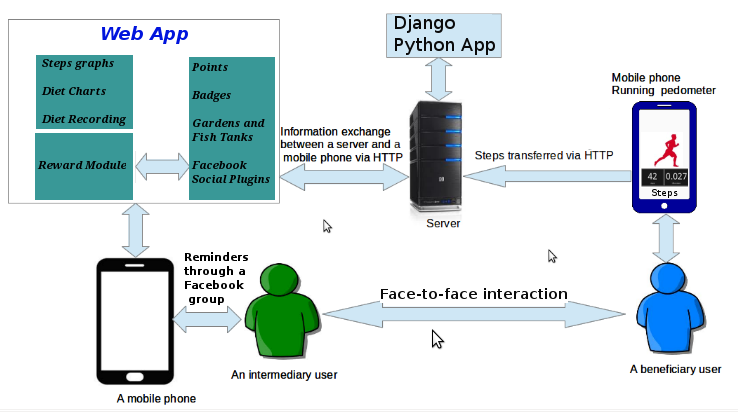
\includegraphics[width=0.8\textwidth]{Figures/prototype_1a.png}
    \rule{35em}{0.5pt}
  \caption{Information flow in the first prototype.}
  \label{figure:prototype_1}
\end{figure}

I developed a web app using a combination of several web technologies such as HTML, JQuery, JavaScript and CSS on the client side, while I achieved the implementation of the server side using Django Python framework. Sample screen-shots of the prototype are shown in Figure \ref{figure:prototype_1_screens}. 

\begin{figure}[htbp]
  \centering
    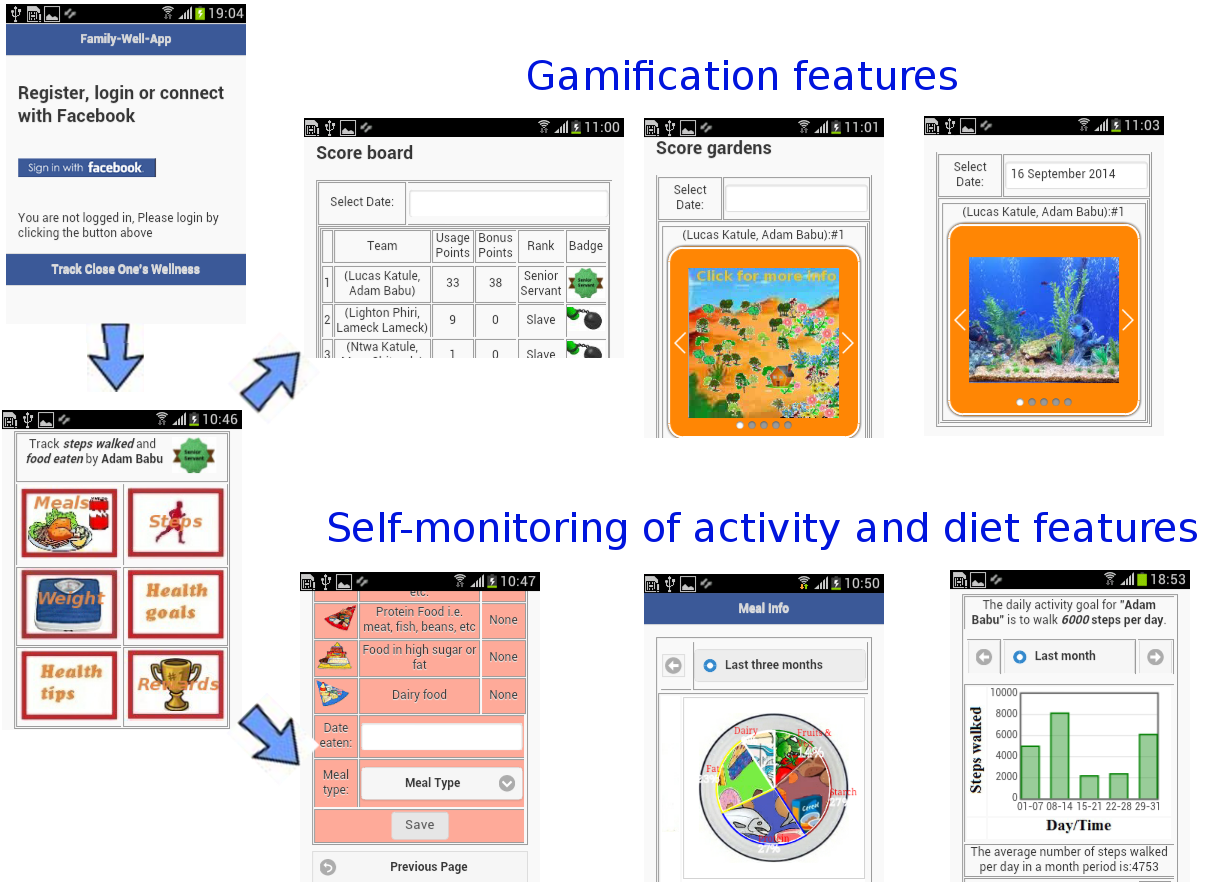
\includegraphics[width=0.8\textwidth]{Figures/Version1/Prototype1Screenshots.png}
    \rule{35em}{0.5pt}
  \caption{Sample screen-shots of the first prototype.}
  \label{figure:prototype_1_screens}
\end{figure}

The system could authenticate users through Facebook accounts of intermediary users. I developed the pedometer app (Figure \ref{figure:pedometer_screen}) in Android environment by extending the open source code downloaded from Github\footnote{https://github.com/bagilevi/android-pedometer}. 

\begin{figure}[htbp]
  \centering
    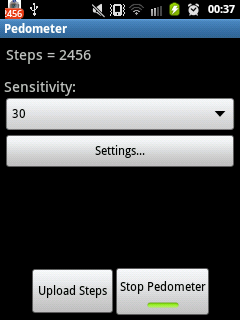
\includegraphics[width=0.3\textwidth]{Figures/pedometerapp.png}
    \rule{35em}{0.5pt}
  \caption{The native pedometer app.}
  \label{figure:pedometer_screen}
\end{figure}

The pedometer code allowed readings from the phone's accelerometer (built-in sensor to detect physical activity) that are above a certain threshold to be detected as bodily bounces from physical activity. The data was then stored in the SQLITE database on the phone. The pedometer app included the capability for transferring data to the server after every 30 minutes, but users could also press an upload button on the pedometer app for immediate transfer of footsteps to the server. The pedometer was not calibrated to differentiate varying intensity of physical activity as it was not an important aspect for this study. A single body bounce was treated as one step regardless of its intensity. 

This prototype aimed at encouraging an increase in physical activity and  a decrease of sedentary behaviours through informing individuals (help-seekers) of their current behaviour trends. In addition, individuals could monitor whether they were eating healthily or not. Some visualization techniques that are similar to this have previously been used  in systems that were designed for direct users such as Fish'n'Steps~\citep{lin2006:fish}, Ubifit~\citep{klasnja2009:using}  and the Few Touch application~\citep{arsand:mobile}. In the reported study in this chapter, the way the fish tank or garden appeared depended on how many footsteps had been captured.  

Another aspect of interface design, was the idea of using a plate to show distribution of meals' nutrition mimicked a practice that was used by dietitians at the hospital where we conducted the contextual enquiry reported on in the previous chapter. In this design metaphor, the amount of each food group that needs to be consumed is presented as a bisector of a pie chart. 
\section{Prototype Evaluation}
There was a slight change of plan  due to contention about the study design and ethical implications when dealing with patients as per requirements of the Faculty of Health Sciences Human Research Ethics Committee (FHS-HREC) of the University of Cape Town. FHS-HREC was interested in having clinical outcomes as one of the expected outputs. These requirements were going to increase the scope of the work, of which the main area of contribution was supposed to be in human-computer interaction. Also, the envisaged technology was only under research; hence it was not expected to be comprehensive enough and ready for any clinical trials even after completion of all evaluations that were meant to be carried out throughout this research. Therefore, I had to look for a different group of participants outside hospital settings. This involved reapplication for ethical approval to an institution body different from the first one that approved the study reported on in the previous chapter (Chapter \ref{contextualenqchapter}). This time the ethical approval was granted by the Faculty of Science Research Ethics Committee (FSREC) of the University of Cape Town (see Appendix B).

In order to evaluate the aforementioned prototype, I recruited participants through help from \textbf{\textit{Mamelani Projects}}\footnote{http://www.mamelani.org.za/}, an NGO
based in Cape Town. This NGO was conducting out outreach programmes on health education in less-privileged communities, and training women on issues of HIV/AIDS, nutrition and gender equality. 

The NGO helped to recruit participants among people who were part of their training in Philippi township. Criteria for recruitment were as follows: (1) participants that were mid-aged and above (contextual enquiry suggested that most prospective beneficiaries could be above mid-aged) and (2) participants who had an intermediary person willing to work with them (someone they trusted or close to them). The NGO identified the targeted participants that met the inclusion criteria. We recruited a total of six adult participants, all of them women above mid-age (\textgreater= 35 years of age). Each of the adults brought one intermediary to form a pair. Three intermediaries were girls between 19 and 23 years of age; the remaining three intermediaries were boys between 14 and 19 years of age. 

In the next step, I informed participants of their rights and that the study will collect their information. Both adults and their respective intermediaries signed consent forms, except those intermediaries who were minors; these signed assent forms that were approved by their parents/guardians. 

The next step entailed training the intermediaries to use the app. I deployed the application in the field from the end of October 2014 to the beginning of December 2014. In order to limit potential complications from deploying the intervention on multiple platforms, each pair of participants was given one Android phone (Samsung GT-S5300) running the pedometer app. I had set each pedometer with the identity of a pair in order to distinguish readings from different pairs. Participants were required to utilize the web application hosted at the University of Cape Town by using a web browser built into their phones. In order to retain participants in the study, each intermediary participant and each beneficiary participant who remained as part of the study received ZAR30 (USD3) worth of airtime every week for the duration of the study. I collected qualitative feedback in the middle and at the end of the study. All names used in the qualitative feedback are pseudonyms to protect the identity of the participants.
\section{Findings}
Observations and qualitative feedback from the six cases/pairs are presented below. The first three pairs were parents working with their children, while the remaining three pairs were an adult working with either a close or distant relative.
\subsection*{\textbf{Pair 1: Mother and Son}}
This pair was a 17-year-old called ``\textbf{Jabulani}'' and his mother ``\textbf{Nandipha}''. Jabulani lived with his mother and siblings. He appeared to be passionate about engaging with a cellphone. Below he describes the intimate relationship he has with his cellphone.

\userquote{\textbf{Jabulani}} {``There is a time I lost my cellphone. It was like the end of the world to me, because I didn't have anything to play with.''}

This shows that a cellphone could be a source of intrinsic motivation for young users in this context. 

He mentioned that he felt happy helping his mother. He also articulated the reason for helping his mother was that he felt it was his duty, since she had taken care of him when he was growing up. 

\userquote{\textbf{Jabulani}} {``I feel happy when I am helping her, because she helped me when I was growing up. So it is my turn to help her''}

\textbf{Nandipha} also felt very happy being helped by her son and said that she thinks her son is more brilliant than her with technology, and that she gets to know things because of him. 

Jabulani and Nandipha were the first to engage with the app for at least three different days. Then all of a sudden, they stopped using it. When I asked them what prevented them from using the app, they replied that, they were more conscious about airtime and so did not log in more often. There were times they ran out of airtime, and thought having more data bundles might solve the problem. Another reason they did not use the app more often was because of a lack of competition from the other pairs and also because they had accomplished the highest challenge within a few days. In the first few days, they were intent on attaining the highest badge. Jabulani said that his mother walked up and down in  order to reach that goal, both having decided to reach that goal in  a week. When they achieved this, the challenge was over for them.

Badges were one source of motivation for this pair. Jabulani was motivated by the badges and he persuaded his mother to work harder so that they could reach the highest badge which was Queen/King.

\userquote{\textbf{Jabulani}} {``We talked, me and my mum, that we must not reach only for today but for the whole week. That was our goal: to reach the queen and the king for the whole week. I remember a day that was the best day. My mum woke up very early to walk around, to go to Philippi Makasikava [a location within the neighbourhood.] just to reach that goal.''}

Jabulani also noticed something on the scoreboard. He and his mother were leading, another team (Pair 3) was in second position, and third position was held by Pair 4. Then after a few days, Jabulani noticed that Pair 4 moved from third position to second position, and he told his mother that ``we must not drop down, because they [Pair 4] are going to reach us''. In that context, competition with others was a source of motivation for Jabulani. Although he was helping his mother, he thought of the winning process as theirs, because he used the word “we” all the time -- he felt that part of the process. Moreover, Jabulani enjoyed the information displayed by a botanical garden and a fish bowl, and he explained why he was so interested in these visualizations. When he was growing up he used to watch cartoons, so when he saw those pictures of trees and fish, he felt he is part of that process of making those images/cartoons. Drawing fish and trees through their team's performance motivated him more and he told his mother that they must have more fish in the bowl.~The idea of fish in the bowl motivated Nandipha to walk more. She did not like to see her bowl empty, so she tried to walk more steps. 

The virtual-pet metaphors such as fish bowls/tanks and garden have previously been utilized in systems that involved only one user interacting with user interfaces in systems such as Fish'n'Steps~\citep{lin2006:fish} and Ubifit Garden~\citep{klasnja2009:using}, the only difference in this context being that the same ideas were extended and tested with two users who were collaborating to attain one objective.
\subsection*{\textbf{Pair 2: Mother and Son}}
``\textbf{Dumisani}'', 14 years of age, lived with his mother ``\textbf{Kholiwe}'' and acted as an intermediary for her. They used the system for the first three days only and then dropped out. Kholiwe said because they were unable to access the system every time they tried. The web page kept giving them time-outs, which discouraged them from trying. But I also noticed that Dumisani was not very familiar with Facebook authentication as he had not had an account before. I created an account for him, but it was not very helpful. I arrived to the decision to use Facebook based on an assumption that all intermediaries already had Facebook accounts, which was not the case. However, despite technical challenges, this pair showed enthusiasm in using the app. Time went by and Fikile never used the web app.
\subsection*{\textbf{Pair 3: Mother and Daughter}}
``\textbf{Zama}'', 20 years of age, was supposed to act as an intermediary for her mother ``\textbf{Fikile}''. Since the daughter appeared to be interested in helping her mother, one would think that intermediation was possible, but they lived in different houses and never used the system at all. There was minimal contact to discuss issues about the system, as Zama was raising a toddler at the time. Fikile appeared to have some expertise in using technology; she was already on Facebook and was interested in learning how to operate the system on her own, but she failed because of her daughter's situation and the fact that the system had been set up to allow a Facebook account for Zama only.
\subsection*{\textbf{Pair 4: Close Relatives}}
``\textbf{Lindiwe}'', a young girl in her early 20s, acted as an intermediary for her aunt ``\textbf{Nceba}'' but they did not live together in the same house. The pair had not been interacting with the application at all, and when I interviewed Nceba to why, her response was that she did not know how to operate it on her own, and her intermediary was not around most of the time. She was curious to access the information but her intermediary was not cooperating, she said she would bring someone else who was also a close relative. The evaluation reached to an end without her having a glimpse of information in the app.
\subsection*{\textbf{Pair 5: Close Relatives}}
``\textbf{Neliswa}'', a 23-year-old girl, acted as an intermediary for her aunt ``\textbf{Nkosazana}''. They lived together in the same house. The pair had not interacted with the application at all, and I never had the chance to find out why, as they were not available for an interview. From personal observation during recruitment, Neliswa appeared to be less interested in the intervention even though she had signed the consent form to participate.  In addition to this, there was one interesting observation about Nkosazana that was reported by another beneficiary participant (Fikile in Pair 3) who was her neighbour: Nkosazana's husband demanded to be the custodian of the study's phone, because he wanted to  control how his wife uses the phone. Patriarchy structures have been suggested as one of the barriers for women in having access to technology~\citep{kumar2015mobile}.   
\subsection*{\textbf{Pair 6: Distant Relatives}}
``\textbf{Nkululeko}'', aged 19, acted as an intermediary for her distant relative ``\textbf{Noluthando}. They did not live close to each other but they saw each other fairly often. System logs showed that they had not been engaging with the application. When I interviewed both of them to find out why that was the case, Nkululeko mentioned a number of things. The first was that he tried to access the application a couple of times but was unable to proceed after login. He was using his personal phone, not the experimental phone that Noluthando had. I checked his personal phone and discovered that his web browser was the problem. But in addition to this, he claimed to be busy with school. Despite his being busy and his phone not being able to support the application, the absence of things like reciprocal benefits and a close social relationship with the beneficiary might have been the reason for his lack of motivation in engaging. The previous user, Jabulani, had trouble accessing the application using his personal phone but he made an effort to access it using the phone given to his mother. So, the closeness/bond between the two members of each pair could be the base for the collaboration to happen. It also made it easier for the intervention phone to exchange hands between members, as a result, intermediaries in such pairs had freedom to access their beneficiary's phone. 
\section{Discussion}
Only two pairs of users engaged with the system for more than two days. Both of these consisted of a beneficiary and an intermediary living in the same house -- mothers working with their sons. One of these pairs was initially very motivated and enthusiastic about the system, but after some time became bored because there was no competition from other teams and they had attained all the challenges within a short period of time. With the third pair, a daughter and her mother were working together but they were not living together, so it was difficult for the daughter to commit to the application. Intermediaries from the remaining two pairs showed little enthusiasm for the project. There are three hypotheses for this lack of enthusiasm: (1) lack of motivation to engage with the system, due to motivational affordances not able to satisfy users' motivational needs; (2) lack of a prior social relationship (a weak bond) between the two users within each pair, hence absence of both empathy and rationale to help by intermediaries; and (3) low frequency of interaction between the two users within a pair due to distance. Chapters \ref{prototype2chapter} and \ref{summativeevalchapter} discuss how both intermediaries and beneficiaries could initiate the intent to use the app; in cases where both members of a pair were motivated, frequent interactions coupled by intents coming from either member, allowed a pair to reflect collaboratively, as a result, this situation led to more engagement than in a situation where members had less encounters. 

Indications point to a prior social relationship being instrumental for intermediaries to perceive value in the act of helping their beneficiary users, in which case the interaction became more meaningful. This is evident for the case of Jabulani, as the rationale for becoming more interested in the intervention was entangled with empathy for his mother and an attempt to nurture their prior social relationship. It was also easier for the two users within a pair to arrange interaction. For the three pairs that consisted of a parent-child relationship (mother and son or mother and daughter), the two members of a pair generally showed an eagerness to work together. For those three pairs without a parent-child relationship, intermediaries showed little enthusiasm in the intervention. Another advantage of a parent-child relationship was in the sharing of phones. It was easier for an experimental phone to move from a beneficiary to an intermediary when a parent and child were involved in a pair. There was a form of trust that existed between the two users with a prior social relationship. This facilitated collaborative reflection which we have already highlighted that it might be important for enhancing user experience. In addition, intermediaries had more authority when they were helping a person who was close to them, as it was seen in the case of Jabulani who desired to see his mother walking more steps. If a pair with a prior social relationship needed to interact with the app, then the frequency of these interactions depended on proximity between the two members of a pair. In instances where they cohabited or lived nearby, it increased the chances of face-to-face meetings and negotiation for interaction. For instance, Zama and her mother Fikile did not cohabit, and Zama had a toddler, which lowered her ability to participate in the intervention. Through interacting with the participants, I observed that, older children tended to be distracted by other activities and were less interested in gamification.  A take away from this observation is that, the less distracted (occupied) the intermediary is, the better the chances for committing to an intervention. As a result of this observation, I tried to put an additional requirement for selecting intermediaries to participate in studies reported on in Chapters \ref{prototype2chapter} and \ref{summativeevalchapter}: preferably, a group of intermediaries who are school going children and cohabit with beneficiary participants.    

A prior social relationship also worked in parallel with the presence of interest in using the app/gamified features. A combination the two factors played a role in  encouraging the two users within a pair to collaborate when they met. For instance, in the case of of Jabulani and Nandipha (mother and son), they discussed strategies to win against other pairs. Although Jabulani was helping his mother, he felt part of the process because he used the word ``we'' all the time. In addition, if intermediaries are motivated, they can become persuaders of beneficiaries with whom they have a prior social relationship, as can be seen with Jabulani who encouraged his mother to walk more. Nandipha was also motivated by gamification, this is shown by an emotional attachment between her and the virtual pet (fish bowl). As a result, the virtual-pet metaphor encouraged Nandipha to be competent, as she attempted to master how to reach the daily-level of recommended physical activity.

To a great extent, the evaluation encountered many hiccups that I could have never anticipated at the beginning. I as the researcher, came to the participants' community as an outsider, hence was not familiar with the context. For instance, on testing the application in the suburb where I was currently living at the time of this study, all features could load without any problems. But after deploying the app to the field, I discovered that there was poor Internet signal, which affected the performance of the app, as a result, some features failed to load when users opened the app. Due to remoteness of the study site, it was difficult to make frequent follow ups and organize meetings with the participants, to discuss any encountered challenges. Challenges in our field work were not specific to this chapter alone, as later chapters (Chapters \ref{prototype2chapter} and \ref{summativeevalchapter}) also continue to bring out more unique challenges; and further discuss in general about challenges of doing field work in the context of ICTD. But it is worth mentioning some of the major drawbacks that affected participation in this evaluation: intermittent Internet connectivity, insufficient airtime, less-motivated intermediaries, and lack of competition/challenges with others in the gamified system. Other factors included how often the two users met (whether they cohabited or they met more often), and untimely reminders. I had very high expectations that Facebook reminders would work for this community, the assumption being that every intermediary would be on, but this was not the case. Some intermediaries had never engaged with Facebook before, and those had were not doing so often as I anticipated. For instance, Jabulani had used Facebook before and was only engaged with Facebook, at most, twice a week. Therefore, Facebook might not be an on-time platform for delivery of reminders or any messages to intermediaries in this context. The presence of above challenges helped in understanding the important contextual factors to consider when setting up an intervention in a low socioeconomic area. 

Despite the above challenges, the one pair that had meaningful engagement with the app, helped me as the researcher to obtain valuable insights about the feasibility of a gamified personal health informatics for intermediated use. The intervention seemed to promote compliance with tracking of physical activity by Pair 1 (Jabulani and Nandipha), however, the pair had a low compliance in the frequency of recording meals consumed by Nandipha. This lack of compliance was due a weak connection between that process and the rewards provided by gamification. As a result, in the second prototype, I did improve this linkage to make pairs of participants to increase frequency of recording meals consumed by the beneficiary.  

Findings from this informative evaluation led to another iteration in the design. It also informed the manner in which I conducted evaluations in chapters \ref{prototype2chapter} (Prototype II) and \ref{summativeevalchapter} (Summative Evaluation). 
%\begin{flushright}
%\end{flushright}

% Chapter 1

\chapter{Prototype II} % Main chapter title

\label{prototype2chapter} % For referencing the chapter elsewhere, use \ref{Chapter1} 

\lhead{Chapter \ref{prototype2chapter}. \emph{Prototype II}} % This is for the header on each page - perhaps a shortened title

%----------------------------------------------------------------------------------------
\section{Prototype Development Iteration II}\label{prototype2descr}
I started the next iteration of prototype development that aimed to improve the first prototype described in Chapter \ref{prototype1chapter} (Prototype I). In the second prototype, the emphasis was more on improving support for the three psychological needs from self-determination theory \citep{ryan2000:self}, which are relatedness, competence and autonomy. I replaced Facebook social plug-ins with features that would allow users to directly comment on or like each other. Facebook social plug-ins failed to integrate seamlessly with the app, since the network signal was poor in the area where I conducted the previous evaluation reported on in Chapter \ref{prototype1chapter}. Therefore, users failed to load them into the app. In addition, the improved system implemented SMS reminders and feedback instead of Facebook-based reminders. The idea in the second prototype was to design challenges that promote collaboration between intermediaries and beneficiaries; as a result, I did improve the design of the challenges to encourage an intermediary and a beneficiary to work together towards the self-monitoring of health for the beneficiary participant. In the evaluation of the first prototype, I observed that collaborative discussions between members of a pair  with prior social relationship, enhanced engagement and made the app more fun to use. Therefore, the design of the second prototype retained the single user interface shared by a pair, to make the collaboration more practical. The new system is shown in Figure \ref{figure:prototype_2_screens}.

\begin{figure}[htbp]
  \centering
    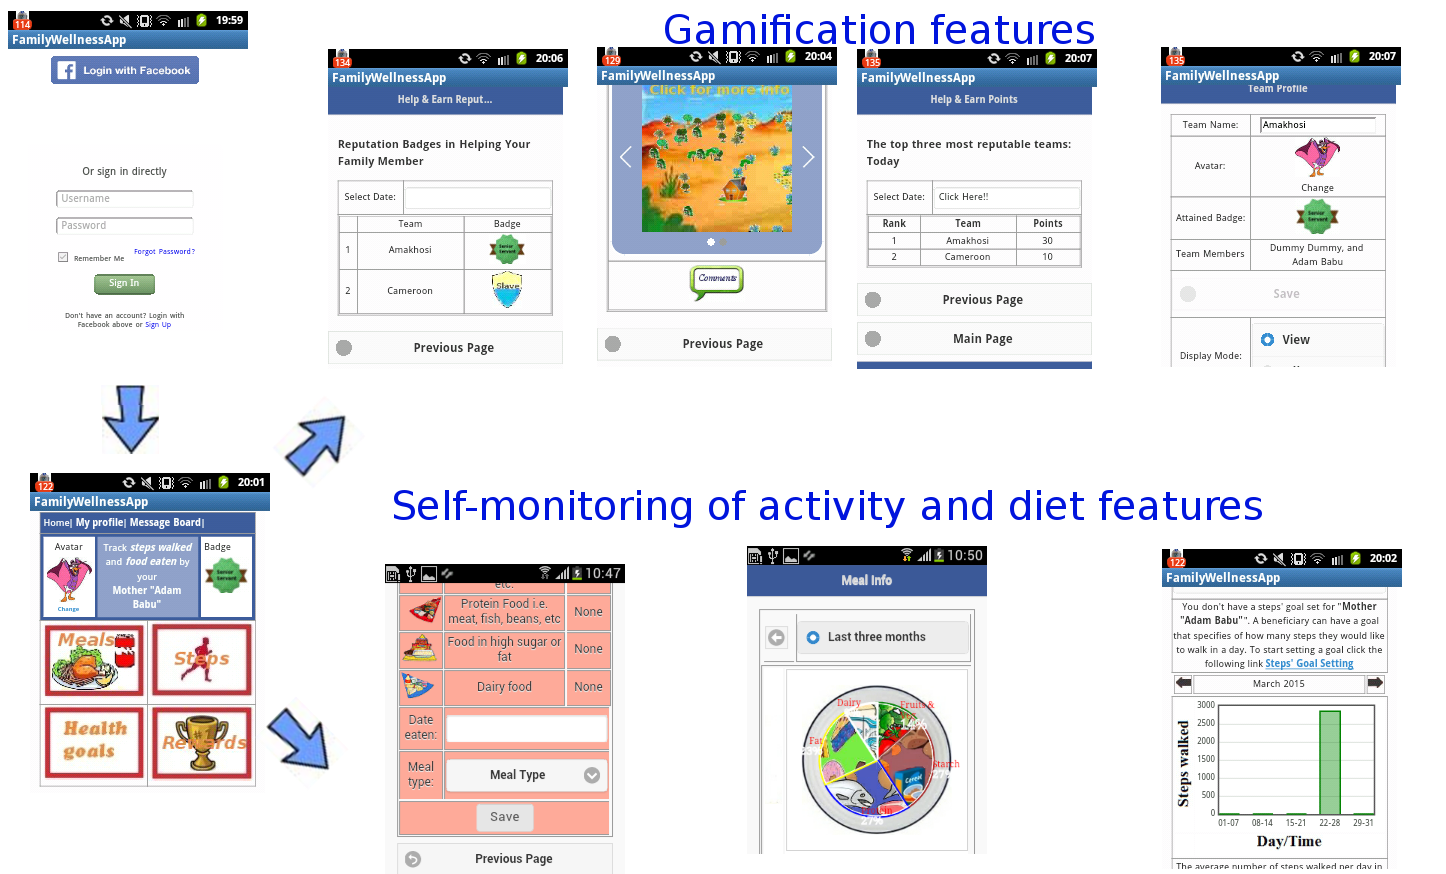
\includegraphics[width=0.8\textwidth]{Figures/Version2/Prototype2Screenshots.png}
    \rule{35em}{0.5pt}
  \caption{Sample screen-shots of the second prototype.}
  \label{figure:prototype_2_screens}
\end{figure}

In this improved prototype, some features remained the same as or slightly improved from, the first prototype. For instance, the journal for
self monitoring of nutrition and physical activity, was only improved to give users the flexibility in navigating across the recorded data by using different intervals of time: daily, weekly or monthly summaries, for physical activity and nutritional components of meals.

This prototype also consisted of a leaderboard as in the previous prototype. In this leaderboard, each team (a pair of users) is ranked based on their points, which are determined using three factors: frequency of app usage, beneficiary's footsteps count, and recorded nutritional components of meals consumed by the beneficiary. However, there is a difference between the leaderboard reported on in the previous chapter and this one: the current leaderboard contains a few information (only displays names and points, for participating teams); in the first prototype, the leaderboard contained points, badges and participant names. Points are more meaningful in a leaderboard as they promote competition with others; badges can be used to promote both competition with self and competition with others. Therefore, I as the developer, decided to separate badges and points to stand independently, on their own interfaces.  

In the improved prototype, badges are awarded sequentially to teams that achieve two important milestones (challenges -- coded in the app): a team must have at least a certain number of both footsteps and days in using the app, that are required to attain a higher badge (by one position) than the current badge. The script that awards teams with new badges was set to run at most once a day and used the predefined challenges similar to the ones in Table \ref{table:badges}; any team that solves the current challenge is then promoted to the next higher badge. These badge-attainment requirements are more stringent than the ones used in the first prototype, where the incremental process was not followed, as a result, teams could skip intermediate badges in between and get to the highest badge that corresponds to their current performance. This made the badge challenge easier to attain within a few days as it was observed in the case of Jabulani and his mother (Chapter \ref{prototype1chapter}). The improved set of challenges required a much longer pair's commitment to the intervention, to reach the highest badge (Queen/King). Therefore, the new rules increased the difficult level of the presented challenges. Each team had their badge displayed in two places: in the top right corner of the main screen and at a separate board that also displayed badges for other teams.
\begin{table}[h!]
  \begin{center}
    \caption{Examples of badge challenges in the app.}
    \label{table:badges}
	\begin{tabular}{|l|l|p{3cm}|p{4cm}|}
		\hline
		Status &Badge &Frequency of app usage (days)&Daily average number of footsteps\\
		\hline
		Queen/King&
\includegraphics[scale = 0.75]{Figures/badges/king.jpg}&18&10000\\
		\hline
		Princess/Prince&
\includegraphics[scale = 0.75]{Figures/badges/prince.jpg}&16&9000\\
		\hline
				Grand Master&
\includegraphics[scale = 0.75]{Figures/badges/grandmaster.jpg}&12&7000\\
		\hline
		 .&.&.&. \\ 
		 .&.&.&. \\   
		 .&.&.&. \\ 
		 .&.&.&. \\
		 .&.&.&. \\
		 \hline
		Servant&
\includegraphics[scale = 0.75]{Figures/badges/servant.jpg}&1&2500\\
		\hline
		Slave&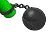
\includegraphics[scale = 0.75]{Figures/badges/slave.jpg}&0&\textless 2500\\
		\hline
	\end{tabular}
  \end{center}
\end{table} 

One observation from the first evaluation (Chapter \ref{prototype1chapter}) is that, the process of recording meals was not as popular as, was the tracking of the steps, because, it did not indicate any pattern in arousing the interest of the participants. One possible reason for this is the weak link between the process of recording meals and the resulting rewards in gamification, as a result, pairs could not offer insights on engagement with this feature, only to focus on the steps. Therefore, I improved challenges for the fish tank and the botanical garden, to bring engagement with the process of diet self-monitoring. The improved design aimed to also promote healthy eating. I made the process of diet self-monitoring more salient by linking it to the vitality of virtual pets (fish and trees): the number of trees in the garden or fish in the tank were determined by the current team's badge and the number of meals recorded. There was a bonus awarded for meals containing portions of fruit and vegetables. This bonus is used to improve the appearance of both plants in the garden and fish in the tank. Therefore, in this new design, steps, frequency of app usage and more specific, frequency of recording meals, all three contributed to both the growth of trees in the garden and fish in the tank; the frequency of app usage and the captured footsteps, contributed indirectly through badges. 

The last additional improvement in the app, aimed to support autonomy: a team is now able to edit their team's name and change their avatar.

I did  specify the rules for engaging with gamification as part of the user manual. But the system also sent periodic SMS hints to pairs, to remind them, what they need to do, to master the presented challenges. These messages were tailored with the name of the intermediary participant. For instance: ``\emph{Tip of the day: Hey Zizile, every recorded meal by your aunt can give you points to buy food for your fish...[Family Wellness App]}''. 
 
\section{Prototype Evaluation Description}
In this evaluation, I had planned to recruit another group of participants. The NGO facilitated access to a group which resided in a different area of Philippi from where evaluation of the first prototype was conducted. The plan, however, did not materialize, as the NGO suggested that we look for a different group, because the group they were working with expressed concerns regarding safety issues after they heard that they were going to be given phones to use throughout the evaluation period. The NGO was concerned about the safety of researchers, since rumours had spread throughout the community that someone was going to bring phones to that area. This posed risks to both prospective participants and the researcher, and highlights the limitations and dangers of doing smartphone-based interventions in low-income areas~\citep{Molapo2015}. 

In order to proceed, I revised the plan, and in the process, found another low-income township called Langa, more modern, not far from the central business district (Cape Town), and safer compared with Philippi. 

A research facilitator who was a resident of Langa helped with the recruitment process. This time, I came up with more stringent recruitment criteria than the previous evaluation (Chapter \ref{prototype1chapter}). I introduced one of the criteria as having intermediaries that cohabit or live near the beneficiaries. Preference was given to schoolgoing children as they were more likely to be interested in gamification. The research assistant managed to recruit a total of nine adult participants for the study: three males and six females, with an average age of 49.3 years (standard deviation of 7.9 years ). Each adult participant brought one intermediary participant and formed a pair. There were three male and six female intermediary participants, with a mean age of 14 years (SD=4.3). Eight of the adults  were relatives/familial relatives of intermediary participants, while the remaining adult was a tenant of her intermediary's grandmother. Eight of the intermediary participants were schoolgoing children.

Prior to commencement of the study, I gave out information about the study to both beneficiary and intermediary participants, informed them that the study's cellphone would be collecting their information related to usage of the app, steps walked, and recorded nutritional components of meals consumed by beneficiary participants. I informed them that the collected information would be transferred to a computer at the University of Cape Town. All participants who were not minors signed informed-consent forms, while minors signed assent forms that were also signed by their guardians/parents.

Once consent and assent forms were signed, one day was allocated to training intermediary participants how to use the app. After the training, I provided each pair with one Android phone (Samsung
GT-S5300), installed with two native apps. The first app was a pedometer (the same given in Chapter \ref{prototype1chapter}), which displayed no useful information other than raw steps data. The pedometer's task was to send these steps to a server so that they could be presented  and viewed in a better format through a web application. The second app provided a link to the web application. One small observation from the previous evaluation reported on in Chapter \ref{prototype1chapter} (Prototype I), it was difficult for users to remember the URL for the web app, therefore a native link provided the easy way to access the app.

In order to encourage participation, each beneficiary participant received ZAR40 ($\approx$USD4) worth of airtime four times in a period of three weeks: ZAR160 ($\approx$USD16) in total. To encourage participation of intermediary participants, the research credited each pair with 300MB of data to use on the Android phone, as it was expected that intermediaries would borrow phones to access other things on the Internet that were beyond the prescribed uses. Providing data bundles was so as to avoid the problem of intermittent usage due to lack of data as observed in the previous chapter.

I deployed the app in the field for three weeks and at the end I conducted an evaluation. The next subsection provides the description of the evaluation.
\section{Prototype Evaluation Methods}
The evaluation relied on two approaches: (1) collecting user logs and (2) interviews. As, all respondents were familiar/comfortable with English, I conducted all the interviews in English. I interviewed a total of three intermediary participants, and five beneficiary participants. These were the only participants that I could reach during the time of interviews. Each short interview lasted for 15 minutes at most. Pseudonyms have been used in findings from the interviews in order to protect the identities of the participants. On reporting the age of participants in interview excerpts, the notation \emph{yrs} refers to years. When the participant's name is introduced or appearing within text (including excerpts) for the first, their age and gender are also mentioned. When participants are mentioned without their age or gender, it implies that they have already been introduced before. 
\section{Findings}
The key findings were based on social technical settings and motivational strategies that influenced usage of the app. Some of the findings from this chapter together with findings from the previous chapter (Chapter \ref{prototype1chapter}) have appeared in a conference paper that I co-authored \citep{katule2016leveraging}.

In this context, intermediaries were very useful in facilitating access on behalf of their respective beneficiary users; hence intermediaries were acknowledged as having expertise that beneficiaries did not have (Table \ref{table:skilledintermediaries}).

\begin{table}[h!]
\renewcommand{\baselinestretch}{1.5}
  \begin{center}
    \caption{Excerpt: an example of how intermediaries trusted as experts by beneficiaries.}
    \label{table:skilledintermediaries}
	\begin{tabular}{|l|C{12cm}|}
		\hline
		No.&Comment\\
		\hline
		1.&\userquote{\textbf{Dlamini}, a male beneficiary, 72 yrs} {``When it comes to the app, I give it to him [\textbf{Vuyo}, a male intermediary, 10 years old]. He is the mastermind on it. All I tell him is just what happened during the course of the day, the meals were as follows, and he is the one that manoeuvres all the stuff.''} \\
		\hline
	\end{tabular}
  \end{center}
\end{table} 

There were two main factors that were crucial in facilitating intermediated use in the context of this evaluation. The subsections below have highlighted these factors.

\subsection{The Role of a Familial Relationship in the Intervention}
As noted in the previous chapter (Chapter \ref{prototype1chapter}), a parent-child relationship may be important in the implementation of such an intervention. In this case, a prior social relationship was also very important. Intermediaries who were working with their parents were eager to support their parents because they cared about them. 

I clustered usage by each pair to its respective relationship type as shown in Figure \ref{figure:relation}. There were three types of relationships: parent-intermediary, relative-intermediary, and not related, with four, three and one as their respective number of pairs. I measured usage within each relationship through three dimensions: (1)~the mean number of days for all pairs; (2)~the average number of sessions per pair; and (3)~the average number of clicks per pair. As a result, I observed more usage for pairs with a parent-intermediary relationship. 
\begin{figure}[htbp]
  \centering
    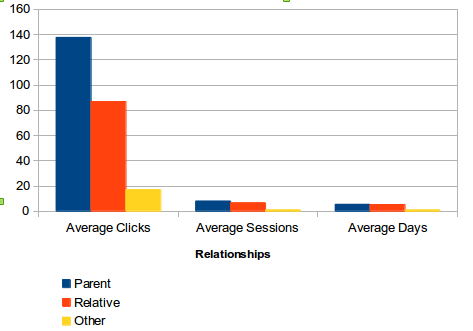
\includegraphics[width=0.7\textwidth]{Figures/relationships.png}
    \rule{35em}{0.5pt}
  \caption{Usage in three groups of relationships~\citep{katule2016leveraging}.}
  \label{figure:relation}
\end{figure}
In the case of parent-intermediary or relative-intermediary relationships, negotiation for interaction that was initiated by beneficiary users was more possible because of the nature of the prior social relationship. In cases of a good prior social relationship, requests from beneficiaries were always successful most of the time. For instance, \textbf{Zandiwe}, \emph{a beneficiary user, a 50-year-old woman}, was working with her sister's daughter. In another case, \textbf{Lulama}, \emph{an intermediary user, a girl aged 20}, was working with her mother, \textbf{Nokhanyo}, \emph{57 years old}. The two cases are presented in Table \ref{table:negotiations}

\begin{table}[h!]
\renewcommand{\baselinestretch}{1.5}
  \begin{center}
    \caption{Excerpts: examples of how a good prior social relationship gave an advantage to beneficiaries when negotiating for intermediated use.}
    \label{table:negotiations}
	\begin{tabular}{|l|C{12cm}|}
		\hline
		No.&Comment\\
		\hline
		1.&\userquote{\textbf{Zandiwe}, a beneficiary} {``I used to call Lindiwe [an intermediary, 16 years of age] like `Lindiwe, there is something that I don't understand'. Or I call her the day before when I walk for a long time, I call her to come and help me some way somehow.''} \\
		\hline
		2.&\userquote{\textbf{Lulama}, an intermediary} {``My mother was the one who was pushing me, let’s do it, let’s do it. And we spent more time together. But we are always together around that time; I do the app at around eight o'clock at night. So we talk more than before because she would ask `How am I doing on this?' ''}\\
		\hline
	\end{tabular}
  \end{center}
\end{table} 

There were instances where a beneficiary user would request assistance at the time when the intermediary was either resting or occupied with other activities or felt that there was no urgency in fulfilling such a request. However, a social relationship still played a role in getting intermediaries to immediately attend to such requests; this was possible, due the empathy on the side of intermediaries; hence such intermediaries had more sense of being accountable to their family members regardless of whether their autonomy was violated or not (Table \ref{table:autonomy_vs_relationship}). The excerpt by Lulama, demonstrates that she was aware that her mother had limited skills in operating technology and it was a sufficient rationale to give that kind of assistance, because she cared for her. 

\begin{table}[h!]
\renewcommand{\baselinestretch}{1.5}
  \begin{center}
    \caption{Excerpts: examples for intermediaries' inclination towards balancing between the need for own's autonomy and the need to preserve an existing relationship with their beneficiaries.}
    \label{table:autonomy_vs_relationship}
	\begin{tabular}{|l|C{12.5cm}|}
		\hline
		No.&Comment\\
		\hline
		1.&\userquote{\textbf{Nokhanyo}, a beneficiary} {``We like to fight each other. Sometimes she [\textbf{Lulama}] is lazy to record. I say to her `come up come up you didn’t do your job'. She would say `I am tired from work'. But she would wake up and do everything for me.''} \\
		\hline
		2.&\userquote{\textbf{Lulama}, an intermediary} {``I am helping her so it [the app] has to mean a lot to me.~I am helping her (Nokhanyo) because she doesn't know anything. She is like `What is this?' This is how you do this. She is like `Ooh okay'. So it [the app] means a lot to me because I am helping someone I care about.''}\\
		\hline
	\end{tabular}
  \end{center}
\end{table}  

Another observation from pairs with a parent-child relationship was that  intermediaries demonstrated a sense of being co-owners of the information from the system, because of being absorbed by the experience of interacting with certain motivational affordances in the app. For instance, Lulama used the terms ``we'' or ``our'' repeatedly to describe actions that needed to be carried out by her beneficiary user as shown in Table \ref{table:coownership}. Here it means such an individual's actions are perceived as belonging to the team and not to an individual only. Such cases demonstrated a sense of collaborative ownership of information in the app, which promoted collaboration in using the app. A sense of collaborative ownership was the result of both prior social rapport and engagement from motivational affordances.

\begin{table}[h!]
\renewcommand{\baselinestretch}{1.5}
  \begin{center}
    \caption{Excerpt: an example of an intermediary showing a sense of being a co-owner of the process and outcome in using the app.}
    \label{table:coownership}
	\begin{tabular}{|l|C{12.5cm}|}
		\hline
		No.&Comment\\
		\hline
		1.&\userquote{\textbf{Lulama}, an intermediary} {``When I saw the garden I was like `yeah, our garden is looking beautiful. Let's do more. Let's take more steps. Let's eat more veggies, because it is the veggies and fruit that are important'.''} \\
		\hline
	\end{tabular}
  \end{center}
\end{table} 
 
From a sense of co-ownership, there was a collaborative reflection. Collaborative reflection happened after negotiation to initiate interactions was successful. Negotiations would be initiated within a pair by either member of a pair. Once a negotiation to initiate interaction was successful, then intermediary users navigated through the app. In the process of navigating through the app, anything intermediaries found interesting would be shared with their respective beneficiary users (Table \ref{table:proximatetranslation}).

\begin{table}[h!]
\renewcommand{\baselinestretch}{1.5}
  \begin{center}
    \caption{Excerpt: an example of how intermediaries enabled proximate translation of intents to interact with the app.}
    \label{table:proximatetranslation}
	\begin{tabular}{|l|C{12.5cm}|}
		\hline
		No.&Comment\\
		\hline
		1.&\userquote{\textbf{Nokhanyo}, a beneficiary} {``I didn't use the app. Lulama used the app. I can't use it. She just shows me and then she presses everything.''} \\
		\hline
	\end{tabular}
  \end{center}
\end{table} 

This kind of interaction sparked a conversation between the two users (members of a pair).~As a result of sharing information between members of a pair, there was a collaborative reflection that increased engagement and promoted a bond between two members of a participating pair through motivational affordances that were either directly situated in the app or indirectly situated in the app (i.e. social comparison among beneficiaries who had formed an informal social support group). Through a collaborative reflection, there were attempts by intermediaries to  persuade their respective beneficiaries to do what would be beneficial in getting virtual rewards for the team (i.e. walking more steps) as shown in Table \ref{table:persuaders}.

\begin{table}[h!]
\renewcommand{\baselinestretch}{1.5}
  \begin{center}
    \caption{Excerpt: an example of how intermediaries posed as persuaders for their beneficiaries.}
    \label{table:persuaders}
	\begin{tabular}{|l|C{12.5cm}|}
		\hline
		No.&Comment\\
		\hline
		1.&\userquote{\textbf{Lwazi}, an intermediary, a boy aged 14 yrs} {``I tell her [his mother] like every two or three days `you must go to town to see if you can find a couple of clothes good for me; you will take the steps also'. She takes the phone with her. She puts the phone in her pocket.''}\\
		\hline
	\end{tabular}
  \end{center}
\end{table}

And such intermediaries did not persuade solely for attaining virtual rewards; they also cared about the health of the people they were helping. This phenomenon was observed in two pairs as shown in Table \ref{table:caretakers}.

\begin{table}[h!]
\renewcommand{\baselinestretch}{1.5}
  \begin{center}
    \caption{Excerpts: examples for intermediaries posing as caretakers for their beneficiaries.}
    \label{table:caretakers}
	\begin{tabular}{|l|C{12.5cm}|}
		\hline
		No.&Comment\\
		\hline
		1.&\userquote{\textbf{Nokhanyo}, a beneficiary} {\enquote{Sometimes she used to shout at me. \enquote{No, no you didn't eat that thing. Tell me what you ate in the morning. I saw you eating this. It seems there is nothing for fruits, peanuts. You must remind me to check you}.}}\\
		\hline
		2.&\userquote{\textbf{Lwazi}, an intermediary}{``It [the app] was really good because my mother was limiting herself on stuff like pies and fat food. I would tell her `Don't eat this; don't eat that'. She wasn't eating much vegetables but I was encouraging her to eat vegetables.''}\\
		\hline
	\end{tabular}
  \end{center}
\end{table}

For those pairs that did not have a parent-child relationship, interactions between members were minimal or absent except for cases where an intermediary was motivated by access to the intervention's phone or motivation affordances provided by gamification. Nevertheless, in such cases a prior social relationship, played a role, i.e. relative-intermediary (child), although it was not as strong as a parent-intermediary relationship. In a parent-child relationship the bond was much stronger to the point where intermediaries had authority in persuading their respective beneficiary users. However, the relative-child relationship was better than the absence of a familial relationship. In such cases of relative-intermediary relationships, intermediaries would still provide infrequent help to their beneficiaries. Where there was no relationship between an intermediary and beneficiary, even infrequent help was not available, e.g. \textbf{Anele} (a beneficiary user, a 47-year-old woman, who was working with the granddaughter of her landlord; hence they did not have a familial relationship. Anele shared her frustrations that the child she was working with was not being cooperative.  Every time she requested help, her intermediary claimed to be busy and kept on procrastinating by saying they would do it the next day, and when that day came it was the same thing. Therefore, a familial relationship was an integral component in mediating motivation of some intermediaries to help in this context.   
\subsection{Sources of Motivation for the Two Sets of Users}
In cases where both users of a pair were motivated to use the app and there was a prior social relationship between them, the pair tended to interact in a more playful manner, which brought the two users closer that they were before using the app. This happened when an intermediary was sharing the information to a beneficiary user. In that process of sharing, the interaction was enjoyable and less tense. The excerpt in Table \ref{table:collaborativereflection} describes how the interaction  between members of one pair was enjoyable when the two users were collaboratively engaging with the app. Lindiwe shows excitement upon seeing steps walked by Zandiwe. 

\begin{table}[h!]
\renewcommand{\baselinestretch}{1.5}
  \begin{center}
    \caption{Excerpt: an example of how collaborative reflection enhanced engagement.}
    \label{table:collaborativereflection}
	\begin{tabular}{|l|C{12.5cm}|}
		\hline
		No.&Comment\\
		\hline
		1.&\userquote{\textbf{Zandiwe}, a beneficiary} {` When she [\textbf{Lindiwe}, a girl aged 16 yrs] got time, when she is done with her homework she comes and sees the app. And then laughs at me like `Yo yo yo [an interjection for Xhosa speakers to express the feeling of amazement by something], you can walk yo yo yo', like `you walked a lot today' and what what [referring to other things said by Lindiwe].''}\\
		\hline
	\end{tabular}
  \end{center}
\end{table}

Also, Nokhanyo mentioned how interaction with her daughter was accompanied by laughter during the exchange of information retrieved from the app. This playful environment fostered relatedness and made it easier for the two users from a pair to collaborate and continue engaging with the app. 

However, in engaging with the app, intermediaries and beneficiaries had different motivational goals. Intermediaries were interested in pursuing a goal related to either steps or eating healthily for their beneficiaries in order to achieve rewards in gamification.~For beneficiaries, the primary goal was to achieve more steps for the purpose of informal comparisons with others or for instrumental value to their health. The subsections below expand further on these different sources of motivation.
\subsubsection{Sources of Motivation in Beneficiaries}
One of the factors that played a role in motivating beneficiaries was informal comparison of steps/diet. In the app, there was no feature that supported direct comparison of steps or diet. Instead, beneficiary participants who knew each other implicitly formed a social support group (Table \ref{table:informalsupport}) . In this support group, they interacted with each other through either face-to-face meetings or SMS/voice. These interactions were centred around comparison of steps or diet among each other. Beneficiaries within social support groups were curious about how others were doing and expressed as much while conversing with the respective intermediary users.

\begin{table}[h!]
\renewcommand{\baselinestretch}{1.5}
  \begin{center}
    \caption{Excerpts: examples for existence of informal social support groups for beneficiaries.}
    \label{table:informalsupport}
	\begin{tabular}{|l|C{12.5cm}|}
		\hline
		No.&Comment\\
		\hline
		1.&\userquote{\textbf{Zandiwe}, a beneficiary} {``We [with Nokhanyo] were talking about what we ate. Like Tuesday I phone Nokhanyo to ask her `Did you eat a lot?'. She said `Not today' But she said she ate a lot the day before. It was Monday.''}\\
		\hline
		2.&\userquote{\textbf{Lulama}, an intermediary} {``She [Nokhanyo] would ask `I wonder how so and so is doing?'. She would ask them when she sees them. She wouldn't ask on the app.''}\\
		\hline
	\end{tabular}
  \end{center}
\end{table}

These kinds of social comparisons led to competition between beneficiary participants. Such competition was a consequence of how the app was utilized in the existing social context and not an intended goal of design, as participants extended comparisons beyond what the design of the app supported. Some beneficiary users had set their targets or goals in order to perform better than beneficiaries from other teams within their social support group (Table \ref{table:comparisonbeneficiaries}).

\begin{table}[h!]
\renewcommand{\baselinestretch}{1.5}
  \begin{center}
    \caption{Excerpt: an example of how comparison for steps within the informal social support group steered competition.}
    \label{table:comparisonbeneficiaries}
	\begin{tabular}{|l|C{12.5cm}|}
		\hline
		No.&Comment\\
		\hline
		1.&\userquote{\textbf{Ndileka}, a female beneficiary user, 35 yrs}
{\enquote{I think I was in competition with steps [she is chuckling]. Because others would have said `Ooh I have walked', maybe we look at the thing [pedometer], it says 1900 steps [referring to steps walked by her peers]. And for me I will say \enquote{No, tomorrow I need to walk more than her because she walked 1900 steps. Then I need to walk 2500 steps}.}}\\
		\hline
	\end{tabular}
  \end{center}
\end{table} 

Also, some beneficiaries became interested in some of the gamification features after \emph{proximate translation by intermediary users} (Table \ref{table:bengamengage}). Therefore, intermediaries needed interpretation of what was going on in gamification in order for them to understand it.

\begin{table}[h!]
\renewcommand{\baselinestretch}{1.5}
  \begin{center}
    \caption{Excerpts: examples for beneficiaries' engagement with gamification through proximate translation of information in the app.}
    \label{table:bengamengage}
	\begin{tabular}{|l|C{12.5cm}|}
		\hline
		No.&Comment\\
		\hline
		1.&\userquote{\textbf{Lulama}, an intermediary} {``She [Nokhanyo] saw the garden. The first day she saw just the house and brownish. She is like `what is this'. I told her. She said `Aha! [expressing
dissatisfaction]. It must look green and healthy'. And then
she saw the garden again and said `It is looking good'.''} \\
		\hline
		2.& \userquote{\textbf{Lwazi}, an intermediary} {``She [his mother] doesn't understand the app. I just tell her that people are having ones twos threes (on the scoreboard and badges) and she laughs.''}\\
		\hline
	\end{tabular}
  \end{center}
\end{table} 

Therefore, the most motivating factors for beneficiaries were steps feedback (for challenging self) and comparison (competition) of steps with others. 
\subsubsection{Sources of Motivation in Intermediaries}
There are several factors that motivated intermediaries to use the app, apart from a prior social rapport. Factors that manifested in participants' responses include gamification features, effect of intervention's phones, and self-monitoring of steps. Some intermediaries nudged their beneficiary
users to do more steps or to eat healthily, so that their pairs would win rewards offered by gamified elements of the web app. The extent of nudging was evident in pairs with a parent-child relationship. Gamification features such as badges, a leaderboard and gardens mediated both competition with other intermediaries and competition with self as shown in Tables \ref{table:intermleadengage}.

\begin{table}[h!]
\renewcommand{\baselinestretch}{1.5}
  \begin{center}
    \caption{Excerpt: an example for the role of gamification in motivating intermediaries.}
    \label{table:intermleadengage}
	\begin{tabular}{|l|C{12.5cm}|}
		\hline
		No.&Comment\\
		\hline
		1.&\userquote{\textbf{Lwazi}, an intermediary}{``The app challenged me to compete [with others] because there was this lady I think it was Lulama. She was getting points and I was really stressed out because she was reaching the amount I was getting, so I was pushing hard to get there. But now I am second. If I was using the app so much, I was going to be number one but I am not using the app so much because my mother is not putting her SIM card on the phone....It's the same like a battle; you are battling with other people. So you must be on your toes with the app and see what is going on with your family.''} \\
		\hline
	\end{tabular}
  \end{center}
\end{table} 

Intermediaries were able to interpret some of the intentional motivational affordances that were aimed at persuading intermediary users to perform certain tasks on behalf of their respective beneficiary users. An example of such motivational affordances is where the size of the fish was related to how often meals consumed by a beneficiary user within a pair were recorded. When \textbf{Lwazi} (an intermediary user) was asked what the size of the fish in his tank was, his response was as follows: \emph{``They were medium sized because I wasn't really feeding them.''} By not feeding them he implied that he was not doing enough to record the meals eaten by his mother. This is an example of a connection that was made between playful interfaces and actual health self-monitoring behaviours. Other examples of how such motivational affordances motivated intermediaries are provided in Table \ref{table:intermgardenengage}

\begin{table}[h!]
\renewcommand{\baselinestretch}{1.5}
  \begin{center}
    \caption{Excerpts: examples of how intermediaries' reacted to challenges.}
    \label{table:intermgardenengage}
	\begin{tabular}{|l|C{12.5cm}|}
		\hline
		No.&Comment\\
		\hline
		1.&\userquote{\textbf{Vuyo}, an intermediary}{``When I had little trees it [the garden] encouraged me to record more meals''}\\
		\hline
		2.&\userquote{\textbf{Lulama}, an intermediary} {``When I saw the garden, I was like `Yeah, our garden is looking beautiful. Let's do more. Let's take more steps. Let's eat more veggies, because it is the veggies and fruit that are important'.''}\\
		\hline
	\end{tabular}
  \end{center}
\end{table} 

The findings also revealed unintentional persuasive effects that resulted from SMS reminders. In one context, three participants (one intermediary and two beneficiaries) were convinced that messages were sent by the researcher (myself). The system auto-generated messages tailored with the participants' names. The three participants perceived them as real messages forwarded by the researcher, who probably was following their performance and was trying to encourage them. For instance, in the case of \textbf{Nokhanyo} (a beneficiary user), every time she received a message she would call her daughter to come and see by telling her that it is from so and so (mentioning the name of the researcher). This caused \textbf{Lulama} (an intermediary user) to panic whenever she heard her mother call her about a received SMS. \textbf{Lulama} kept thinking that she had done something wrong.  In a different scenario, \textbf{Lwazi} (an intermediary user) thought that messages were sent by other participants through a message board that was on the app. Therefore, he passed these reminders on to his mother, saying that people were reminding them about eating healthily, and the mother always responded with laughter. \textbf{Lwazi} used these messages to encourage his mother to walk more steps and eat healthily.  

Apart from gamification features, the phone motivated intermediaries to participate, especially those who had a prior social relationship with their beneficiaries. Intermediaries were involved in tasks that were non-prescribed in the course of carrying out tasks within prescribed use. For instance, two intermediaries aged 10 and 14 had installed games on the intervention's phones that their parents had.  In another case, an intermediary user called \textbf{Lindiwe}, lived a distance from a beneficiary user \textbf{Zandiwe}, but she came all the way to use the phone and to interact with gamification.~\textbf{Zandiwe} was \textbf{Lindiwe}'s aunt (Table \ref{table:phoneeffect}).   

\begin{table}[h!]
\renewcommand{\baselinestretch}{1.5}
  \begin{center}
    \caption{Excerpt: an example for the effect of the study's phone in increasing intermediaries' engagement.}
    \label{table:phoneeffect}
	\begin{tabular}{|l|C{12.5cm}|}
		\hline
		No.&Comment\\
		\hline
		1.&\userquote{\textbf{Zandiwe}, a beneficiary} {``\textbf{Lindiwe} likes the phone too much. She is always here after school. She lives with my sister on the other side and she comes here every day. Sometimes I call her to come. We are closer than before. We always talk about the app while other people (relatives) are around. These people also got interested''} \\
		\hline
	\end{tabular}
  \end{center}
\end{table}

There was also the novelty effect of the self-monitoring tasks (diet's pie chart and steps' bar chart). Some intermediaries were excited to see visualization of information about people they cared about. For instance, one 10-year old intermediary, mentioned that steps were the most interesting of all the features. 

\subsection{Perceived Value in Using the Prototype}
The beneficiaries said they had gained knowledge about living a healthy lifestyle (Table \ref{table:benknowledge}).

\begin{table}[h!]
\renewcommand{\baselinestretch}{1.5}
  \begin{center}
    \caption{Excerpts: examples of how the app improved beneficiaries' knowledge.}
    \label{table:benknowledge}
	\begin{tabular}{|l|C{12.5cm}|}
		\hline
		No.&Comment\\
		\hline
		1.&\userquote{\textbf{Zandiwe}, a beneficiary} {``There are a lot of things I didn't know I now know, like how to eat. I know walking is very important. Because, you know, I am fat. When I stay on the bed the whole day, my blood doesn't circulate.''}  \\
		\hline
		2.&\userquote{\textbf{Ndileka}, a beneficiary} {``The app helped me because sometimes you don't realize you eat more carbohydrate than fruit. You just eat bread but you don't know that bread is carbohydrate. So when it says a large amount of carbohydrate, you know I am eating a large amount of carbohydrate. You think `Now I must eat more fruit than meat or less meat'. So for me automatically it helped me to think that I need to eat a large amount of fruit.''}\\
		\hline
	\end{tabular}
  \end{center}
\end{table} 

The case of Ndileka above is referred to as cognitive dissonance. This is why self-monitoring is so important: it shows an individual if there is a discrepancy between their beliefs and their actions. Cognitive dissonance supports individuals to restore consistency between beliefs and actions~\citep{Oinas-kukkonen:psd}.

Intermediaries who engaged with the app also reported that their beneficiaries had become more knowledgeable about living healthily. 
\section{Discussion}
Two important aspects of the findings are worth discussing in this subsection: the importance of a familial relation in user experience and variation in motivational needs of the two sets of users.
\subsection{Familial Relationship in Increasing Users' Engagement} 
The kind of social rapport that proved to be of great importance was a familial relationship, especially a parent-child relationship. The value of this relationship can be perceived as a social support from within the family that is available for beneficiaries. This relationship created a conducive atmosphere for motivational affordances to foster collaboration between an intermediary user and a beneficiary user. A familial relationship helped even in areas of competing needs between intermediaries and their beneficiaries. An important take away out of this observation is how the competing needs from individual members of a pair were inherently harmonised through an existing structure: a social relationship. Structuration theory by~\cite{jones2008giddens}, discusses how recreation of societal structures can be challenged by contradiction and conflict; and in a situation where conflict does not emanate as a result of contradiction, it is because actors are aware of both their differences and motivated to work on them. If we refer to excerpts of \textbf{Lulama} and \textbf{Nokhanyo} in Table \ref{table:autonomy_vs_relationship} above, where \textbf{Nokhanyo} felt of not ready to help because of the timing (her being exhausted after work), but at the end she always agreed to help, one can view our two users (the intermediary and the beneficiary) as a community where members contradict each other concerning the right time for collaborating in using the app, but are always able to reach a consensus, because, their existing familial relationship takes precedence to motivate them to do so. 
  
Through motivational affordances, an interaction was perceived more as a collaboration between two people with one goal than as an intermediated use where one person was only assisting the other person with his/her information need, but with no ties to the information being shared. In this context, intermediaries who engaged with the app became attached to the information that was being shared with their respective beneficiary users.

External sources of motivation such as phone effect and gamification could enhance an existing familial relationship, as the findings suggest. Perceived relatedness between family members increased, and familial relationships created an opportunity to utilize young family members as persuaders for behaviour change. These intermediaries could create intents to persuade. This approach becomes impractical in the absence of a prior social rapport between members of a participating pair. Pairing users (an intermediary and a beneficiary) who have a familial relationship intensified value of the intervention more than pairing individuals with no familial relationship or bond. This approach was quite different from existing approaches in ICTD context.  For instance, there is a project in India that leverages trust between community health workers and expectant mothers for  persuasion~\citep{ramachandran2010mobile,ramachandran2010research}, and this trust is based on persuasive information that community health workers (CHWs) possess on their phones. Therefore, the prior social rapport is relatively weak, and the  influence of these CHWs can be limited to infrequent visits, and much of the persuasive strategy relies on the messages possessed by CHWs \citep{katule2016leveraging}. 

\subsection{Parallel Persuasion of the two Sets of Users} 
Apart from the prerequisite of a prior social relationship, motivation strategies are important as they appeared to strengthen what already exists, the social relationship. Intermediaries and beneficiaries had different motivational needs when engaging with the app. Intermediaries focused on the gamification part as their primary objective. Steps and meals were secondary objectives, since they were somehow linked to the gamification part. Beneficiaries considered steps and meals as their primary objective. Intermediaries competed for points on the leaderboard but beneficiaries competed for the number of steps walked or healthy meals. Therefore, in this context we have two sets of users that we need to persuade differently, since they have different objectives. Motivational strategies for the two users need to be examined separately, and a designer has to come up with an optimal strategy that will combine motivational strategies for the two groups. An understanding of context is crucial and this has been emphasized by~\cite{Oinas-kukkonen:psd} and \cite{Oinas-Kukkonen:foundation}. 

If we delve into the sources of motivation by intermediary users, one can see motivation is twofold. The first dimension has an aspect of ego involved and the second dimension with an aspect of task-mastery climate. The ego involved aspect is exhibited through review of statements by the following two intermediary users, \textbf{Lwazi} and \textbf{Lulama}. Let's refer to one excerpt by \textbf{Lwazi} which mentioned being stressed upon seeing others coming to the top of the leaderboard. If one interprets that statement through the view of internalization of behaviour regulation discussed in the literature review chapter, the above scenario promotes introjected regulation, where ego is involved; hence usage in such context may appear to be influenced by attempts to outperform others. Also, the same emphasis on outperforming others is exhibited by \textbf{Lulama}. The aforementioned comparisons were with respect to the leaderboard. The aspect of motivation that focuses on problem solving or task mastery is demonstrated in the excerpt by \textbf{Lulama} where she explains the discussion with her mother (\textbf{Nokhanyo}) about the meaning of a garden. From this conversation, \textbf{Nokhanyo} emphasizes that their garden must look green. Also, in some of \textbf{Lulama}'s conversations, she keeps on emphasizing making their garden green by eating more vegetables. Therefore, both \textbf{Lulama} and \textbf{Nokhanyo} are able to make a connection with what they need to do in order to master the task of making the garden greener.

In the next chapter (Chapter \ref{summativeevalchapter}), I have expanded the discussion on the two aspects of motivation: one of which promotes ego-involved climate and the other task-mastery climate. Also, the conclusion chapter (Chapter \ref{discussionchapter}) attempts to collate the discussion from all three evaluations in order to broaden the discussion about the implication of this specific finding to the design of gamification.
 
\begin{flushright}
\end{flushright}

        % Chapter 1

\chapter{Summative Evaluation} % Main chapter title

\label{summativeevalchapter} % For referencing the chapter elsewhere, use \ref{Chapter1} 

\lhead{Chapter \ref{summativeevalchapter}. \emph{Summative Evaluation}} % This is for the header on each page - perhaps a shortened title

%----------------------------------------------------------------------------------------
\section{Recruitment of Participants}
With the help of one research assistant and her team (one female field worker who also became one of the adult subjects in the study), I managed to recruit a total of 14 adult participants (beneficiary users) through convenience sampling. By the ``researcher'', in the context of this chapter, I mean myself. In cases where I use ``we'' within text, it implies the researcher and research assistant's team collaborated in doing the work. The research assistant's team approached potential participants for the study at the beginning of  October 2015, and recruited participants from two townships in Cape Town, namely Langa (where the research assistant resided) and Athlone (where the field worker resided). The research assistant coordinated the process while the field worker assisted her. Out of 14 adults, Langa had five, while in Athlone there were nine. There was only one male out of 14 adult participants. It was easier to  recruit females than males, as females were more eager to participate than males; this resulted in a gender imbalance among adult participants.  The study in Chapter \ref{prototype2chapter} also showed this trend of gender imbalance, with more females present. The average age of these adult participants was 44.21 years, with a standard deviation (SD) of 9.99 years. The age range was between 26 and 60 years. The highest education level among adult participants was secondary school, while the lowest was the last grade of primary school. 

The research assistant's team notified adult participants before recruitment that one of the requirements to be part of the study was to have a family member, preferably a schoolgoing child, willing to be part of the study. Each adult participant we recruited elected/brought one of their children/grandchildren to act as their intermediary user. The two people, an adult and a child, formed one pair of users. As a result, we had 14 children in the study. Thirteen adult participants teamed up with their children, and the remaining one adult teamed up with her grandchild. Child participants had a mean age of 15.42 (with a standard deviations of 2.06 years), and the age range of child participants was between 12  and 20 years. There was a gender balance among intermediary participants. 

I visited the two research sites on separate occasions (days) to talk to all participants (adults and children). In these meetings, I gave out detailed information of what the study was about to both intermediary and beneficiary participants. I informed them about the different ways I would be collecting data. The data collection approaches included usage logs, questionnaires and interviews (see more details in section \ref{datacollect} -- Data Collection and Analysis). All the beneficiary participants signed informed consent forms agreeing to be part of the study. Since all intermediaries were under 21 years of age (the legal age for giving consent in South Africa is 21 and above), they signed assent forms which were also signed by their respective parents/guardians who were part of the study.

I allocated one day for training all intermediary participants how to use the Family Wellness app. I conducted training in Athlone (one of the research sites), and the research assistant and her team organized transport for children from Langa (the second site) to be able to attend this meeting. The reason we brought the children together was, firstly, to let them become acquainted with each other (this would be instrumental in gamification). Secondly, it was a good idea to train all intermediary participants at once so that they could start using the Family Wellness app immediately after the training. During the training, each intermediary participant/user received a user manual. After the training, I assigned one Android phone (Samsung GT-S5300) to each pair of participants; children collected these phones on behalf of their parent or grandparent. In each phone, I had installed two native apps on each phone (same apps used in Chapter \ref{prototype2chapter}): the pedometer app and the main `Family Wellness app. The Family Wellness app loaded all its content from a web application, which I hosted at the University of Cape Town. There were two versions of the web app, and I have described the details of these two versions in the Experiment Design section (\ref{exp_design}) below. Each beneficiary participant had to carry the  pair's assigned phone in order for the pedometer app to count their footsteps. Participants had six weeks to use the two apps (main app and pedometer).~Each pair of participants provided the phone number of the SIM card that would be inserted into their given Android phone. I allocated 1.3GB of data to each SIM card, and each beneficiary participant was given a total of ZAR240 ($\approx$ US\$20) for the duration of the study. This amount covered compensation for participants' transportation and time spent on data collection activities such as questionnaires and interviews. The details of the experiment are outlined in the next section. 

\section{Experiment Design}\label{exp_design}
The research objective was to evaluate the effectiveness of gamification in promoting intermediated use in the context of personal health informatics. Therefore, the experiments entailed comparisons between an app that was not gamified and a gamified app. The non-gamified app (the logbook app) was simply a diary/journal part of the prototype described in Chapter \ref{prototype2chapter} -- it enabled pairs of participants to track both the nutritional components of the meals a beneficiary participant consumed and the footsteps of the beneficiary member. The second version of the application was an extension of the logbook; it included all the features of the logbook with the addition of a rewards/gamified subsystem. The details of the gamified subsystem have also been provided in the previous chapter (Chapter \ref{prototype2chapter}). I carried out the experiments from mid-October 2015 to the end of November 2015.

I opted to use the ``within-group'' approach for the experiment design. In this approach there are no fixed control/intervention groups, as the same group of subjects have a chance to experience both control and intervention conditions. The rationale for choosing this design approach was that it reduces interference from confounding factors. The second benefit is that it reduces the cost of recruitment, as the same group is observed in both control and intervention conditions. This approach could also be of benefit in ICTD: recruitment of participants is one of the daunting tasks in ICTD studies~\citep{anokwa2009stories,ramachandran2010research} and this may compromise the rigour of such studies~\citep{ramachandran2010research}. The within-group approach offers benefits in terms of increasing the power of a study by using only half the number of subjects/participants that would have been required in a typical control/intervention study.

I created two experimental conditions one referred to as the logbook condition and one referred to as the gamification condition, and used the same group of subjects for both conditions. There is a caveat in using this approach: the learning effect could affect the rigour of the findings  if all participants start together in one experimental condition and thereafter switch to the other experimental condition. The learning effect would favour any experimental condition that comes first (predecessor), and disadvantage the one that comes last (successor). I dealt with this particular issue by creating experimental sequences, as highlighted in the next paragraph. 

I divided pairs of participants into two groups, the difference being the order in which experimental conditions started and finished.  I referred to each of these modes of starting and finishing as an experimental sequence. Therefore, both groups had a unique experimental sequence. I labelled these two groups ``LG'' and ``GL''.  In the LG group, pairs of participants started with the logbook condition and later switched to the gamification condition. In the GL group, pairs of participants started with the gamification condition and later switched to the logbook condition. I designed the switching of experimental conditions to happen at the midpoint of the experiment. These experimental sequences prevented the learning effect from affecting individual experimental conditions. The objective was to cancel out the learning effect, as each experimental condition was present before midpoint and after midpoint. One drawback of the within-group approach is that it makes the duration of experiments much longer, and this can be tiresome for research participants. However, this was an added advantage for this particular research, since the study was trying to understand any differences in sustained usage of a system using logbook and a system using gamification.

I randomly selected and assigned seven pairs of participants to the LG group, while the remaining seven pairs went to the GL group. Initially the plan was to have the time spent on each experimental condition be three weeks, but phase 1 had extended beyond its allocated block of three weeks up to the fourth week, as pairs of participants were not available for midpoint assessments at the end of the third week. Therefore, I carried out the midpoint assessment at the end of the fourth week. After the assessment, pairs that were using the gamified app switched to using the logbook app, and vice versa. It was not feasible to extend phase 2 to four weeks as in phase 1, because it was approaching December when most people travel for holidays; gathering participants during that time would have been impractical. This shortened the duration of phase 2 to two weeks. These kinds of eventualities are common in field research within the ICTD context. Researchers have argued that even though eventualities may appear to affect the rigour of research, such compromises offer benefits as they tend to preserve contextual interactions which are key to facilitating an intervention~\citep{anokwa2009stories,ramachandran2010research}. Through the course of doing the series of studies reported on in previous chapters up to the current reported study, not everything went according to plan, and compromises and constant negotiations had to be made; these contextual aspects were vital in making this intervention/research a success. Compromises on the rigour of the methods, and how it offered benefits in terms of preserving contextual factors, played an important role in this study. Examples of negotiations were on issues to do with recruitment of participants, and location (meeting points for interviews) and the availability of participants -- interaction between space and time. The aim of this study was not to make any generalization based on statistical tests, but rather to garner insights on human factors on intermediated use when utilizing gamification.  As a result, the takeaways and contribution made by this study are still valid when considering the arising need to understand and preserve the social relations that were crucial in the execution of this field work.
\section{Data Collection and Analysis}\label{datacollect}
I carried out data collection through a triangulation of the application's usage logs, questionnaires and interviews. Questionnaires and usage logs resulted in the generation of quantitative data, while interviews yielded qualitative data. Triangulation of different methods is important when doing research in ICTD, as it strengthens the reliability of the findings~\citep{burrell2009constitutes}.

I analysed quantitative data using both descriptive and inference statistics. Before each inferential statistical test, I tested data points to see if they followed normal distribution. The test that I applied to check for normality was the \emph{Shapiro-Wilk Normality Test}\footnote{http://sdittami.altervista.org/shapirotest/ShapiroTest.html}. I have outlined my reasons for choosing specific statistical tests below.
\begin{enumerate}[label=(\alph*)]
\item  Part of the quantitative data consisted of sets of data with paired samples (two dependent samples) used for analysis. On deciding what statistical test to use, the first step was to test the normality of the difference between repeated measures of each data point. If there was no normality, I would apply a log transformation on the original data, and repeat the normality test. For cases where the data assumed normality, I used parametric tests such as the student-t test with repeated measures. All the sets of paired samples achieved normality on either the original data or transformed data; as a result, non-parametric tests where never used in cases of all sets of two dependent samples.
\item Quantitative data also consisted of sets of data with three dependent samples. In the first step, I paired each sample to one sample from the same set. This process created three pairwise samples. Then  I used the same procedure to check for normality in two dependent samples. In all cases where there were three dependent samples, there was normality on the original data; hence the data did not need any transformation. As a result I ended up using one-way analysis of variance (ANOVA) with repeated measures in all cases where there were three dependent samples.  
\item The third part of the quantitative data sets consisted of two independent samples. I did the normality test on each independent sample. In the absence of a normal distribution in any of the two independent samples, a log transformation was applied. In some cases, data followed normal distribution. In such cases, I used the student-t test with no repeated measures. There was one case of two independent samples that did not adhere to the requirement of normal distribution on either original data or transformed data. In that case, I resorted to using the Mann-Whitney U test -- a non-parametric test\footnote{Mann-Whitney test, a non-parametric test for independent samples}. 
\end{enumerate}
The next subsections provide details of the three data collection methods used in this study.
\subsection{Family Wellness App Logs}
\subsubsection{Generation of Usage Logs}
The web application captured usage logs on the client (user) side through JavaScript events. The app generated events when users touched/clicked links that loaded features/functionality on the app. Asynchronous JavaScript (AJAX) transferred all events to the server for storage on a database, after wrapping them into JSON (JavaScript Object Notation) format. Each object mapped a pair's identity to events in order to know to whom events belonged. Figure \ref{figure:events_logs} shows the logical organization for capturing, transferring and storing events.
\begin{figure}[htbp]
  \centering
    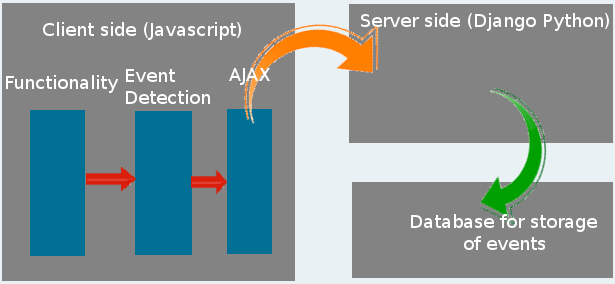
\includegraphics[width=0.6\textwidth]{Figures/events_capture.png}
    \rule{35em}{0.5pt}
  \caption{Generation of usage logs.}
  \label{figure:events_logs}
\end{figure}
Before sending out events, the client application stored them temporarily   until the user moved from one functionality to the other. Then AJAX would send out past events that the client program had already stored in its variables. Due to this delay, the server program was not recording events in real time. This approach of delaying until the user accessed the next feature was intentional in order to minimize the frequency of data transfers between clients and server. This delay did not affect the ability to understand the usage behaviour pattern. 

I chose not to capture the client's clock time on the client side during the capturing of events, because recording the phone's time on the client side had its limitations. There were periods during which the dates on the experimental phones were not correct. I had learned in previous studies (Chapters \ref{prototype1chapter} and \ref{prototype2chapter}) that participants had a tendency of removing SIM cards from their phones, and this would require removing the batteries. After removal of its battery, a phone would lose its clock time. If a user then tried to access the app immediately, time recordings would be incorrect; for instance, the Android phones used for the experiments would set date and time to the default one from the manufacturer. I noticed this pattern by looking at the logs from a pedometer: there were times when the pedometer reported a few incorrect time readings. I confirmed this behaviour of changing SIM cards during interviews reported on in Chapters \ref{prototype1chapter} and \ref{prototype2chapter}. Because of the above stated reasons, I made a decision to capture the time of events on the server side. 

Once events arrived on the server side, the server program (written in Python) would attach on arrival time and store those events in a database. Therefore, the database kept information such as when there was user activity on the app, which pair was accessing the app at that time, and what functionality/feature a pair accessed. The system also categorized events into their respective experimental conditions.  
\subsubsection{Analysis of Usage Logs}\label{log_analysis}
Through the analysis of events that the app was able to capture, I was able to synthesize usage into two useful dimensions: (1) the number of usage sessions of each pair of participants; and (2) the number of views of certain features by each pair of participants, which I will refer to as the ``number of impressions''.

I defined a new session as starting when user activity on the app was detected after an absence of any activity by that particular user/pair in the past one hour or more. The term ``impressions'' is commonly used in social network platforms (e.g. Instagram) to describe views on status updates by userz (things posted by users e.g. text, photos, etc.). In this context, I define impressions as the number of times a certain feature was viewed by a pair. If multiple clicks by one user/pair on one feature happened within an interval of less than one minute, they were grouped as a single impression. If clicks on the same feature differed by a minute or more, I then considered the current click to be a new impression while the previous click belonged to the previous impression. If the time difference between clicks on the same feature was beyond one minute, then it was assumed that the user had gone away or moved to a different feature and was coming back to this feature for another series of clicks. The purpose of computing a pair's total impressions on each feature was to understand where users of the app were likely to go among the many options of gamification features, namely leaderboard (score board), score badge, botanical garden and fish tank (fish aquarium). 
 
I conducted two major analyses of usage logs by using data on number of impressions and sessions. 
\subsubsection*{Comparison of Usage Sessions Between Logbook and Gamification.}
This particular analysis was twofold.
\begin{enumerate}[label=(\alph*)]
\item \textbf{Comparison of Daily Total Sessions Between Logbook and Gamification}
\end{enumerate}
In the first part of this comparison, I obtained the daily total number of sessions in each experimental condition, through adding sessions from all users in an experimental condition. I repeated this process for all 41 days of running the experiment, using the format of Table \ref{table:totaldailysessions}. As the result there were 41 data points. I then compared daily total sessions of logbook and gamification. I treated each experimental condition as an independent variable. I also treated the total number of sessions from all users in a particular experimental condition as a dependent variable.    

\begin{table}[h!]
  \begin{center}
    \caption{An example of total daily sessions from each experimental condition.}
    \label{table:totaldailysessions}
	\begin{tabular}{|l|l|p{6cm}|}
		\hline
		Day&Daily total of logbook sessions&Daily total of gamification sessions\\
		\hline
		Day 1&X&Y\\
		\hline
		Day 2&......&...... \\
		\hline
		.&.&. \\ 
		.&.&. \\   
		 && \\  
		.&.&. \\ 
		.&.&. \\ 
		\hline
       	Day 41&U&V \\
		\hline
	\end{tabular}
  \end{center}
\end{table}

The statistical test that I applied to do the comparison was the Mann-Whitney U Test. I highlighted at the beginning of this section (\ref{datacollect}) how arrived at the decision of choosing one among different tests in each case of inferential statistical analysis. 
\begin{enumerate}[label=(\alph*)]
\setcounter{enumi}{1}
\item \textbf{Comparison of Sessions Between Logbook and Gamification in Each Pair}
\end{enumerate}
I conducted the second comparison between sessions in logbook and gamification at the level of individual pairs of participants. In this comparison, I was looking at how each pair performed in logbook and gamification (i.e. repeated measures for usage during logbook and usage during gamification by the same pair of users). The number of weeks spent on the experiment prior to the midpoint assessment (four weeks) was not the same as the number of weeks spent on the experiment after the midpoint assessment (two weeks). Therefore, it was not fair to compare between an experimental condition that was available for four weeks and an experimental condition that was available for only 2 weeks. For instance, if a pair had started with logbook, they then spent four weeks in logbook and two weeks in gamification. The reverse applies for a pair that started with gamification. In order to make the comparison of the number sessions by the same pair of participants in the two experimental conditions fair, I opted to use a relative (normalized) number of sessions  as a unit of measurement. The formula I used for the normalized number of sessions is as shown below,
\begin{mdframed}[style=MyFrame]
$$T_{mj}=S_{mj}/D_{mj}$$
\end{mdframed}
\textbf{where}:

$T_{mj}$ is the number of sessions per day for a pair $m$ in experimental condition $j$,


 $S_{mj}$ is the total number of sessions for a pair $m$ in experimental condition $j$, and

$D_{mj}$ is the total number days on which pair $m$ could access experimental condition $j$ (27 days $\approx four$ weeks if the experimental condition started before midpoint, and 14 days = two weeks if the experimental condition started after midpoint).
%\noindent

I formulated a hypothesis with the aim of understanding the difference in usage sessions for the same pair of participants, when in logbook and when in gamification.

\begin{enumerate}
   \item{Hypothesis 1}
      \begin{itemize}
       \item{H\SB{0}}: There is no difference in the normalized number of sessions of a logbook app and a gamified app
       \item{H\SB{A}}: There is a difference in the normalized number of sessions of a logbook app and a gamified app
      \end{itemize}
   \end{enumerate}
   
I made a decision to exclude four pairs in testing the aforementioned hypothesis. These were pairs that faced hurdles when utilizing the app as a result of technical glitches. Technical glitches affected their performance in terms of usage sessions. Table \ref{table:usageproblems} provides a list of excluded pairs. 

\begin{table}[h!]
  \begin{center}
    \caption{Excluded pairs as the result of technical glitches.}
    \label{table:usageproblems}
	\begin{tabular}{|l|l|l|p{6cm}|}
		\hline
		&Pair&Group&Problem\\
		\hline
		1&Pair-A&GL-sequence &App failed to load due to poor Internet connectivity and malfunctioning of the phone.\\
		\hline
		2&Pair-B&GL-sequence&This pair didn't have data bundles due to misallocation. \\
		\hline
		3&Pair-C & LG-sequence& Their pedometer didn't transmit steps throughout the duration of the study.\\
		\hline
		4&Pair-D & LG-sequence& Pedometer worked for a while before it stopped transmission of data.\\
	\hline
	\end{tabular}
  \end{center}
\end{table}

For \textbf{Pair-A}, the app failed to load every time the intermediary user tried to use it. The intermediary user from this pair sent a message to the researcher, complaining that the app was unstable as he could not start it most of the time. After a follow-up, I observed that in the house where this particular pair lived, there was poor Internet signal. Hence the app failed to load most of the time and this frustrated the intermediary user. In addition to that, the device itself appeared to have problems, because the intermediary participant reported that all the installed intervention's apps were misbehaving. Majority of the intervention's phones were not new, as they had been used before by other researchers to conduct their experiments. 

For the second pair (\textbf{Pair-B}) in Table \ref{table:usageproblems}, I had sent Internet data bundles to the wrong phone number. I was using Internet banking to buy Internet data and send them to individual phone numbers. In this case, the pair provided a phone number of a SIM card that belonged to a relative: they had put into the experimental phone a SIM card with a phone number that was different from the one they provided to the researcher during the orientation/training. I did this misallocation of Internet data to the wrong phone number at the beginning of the experiment, which the participants did not report on time. When I met them for interviews they claimed they had not received data bundles. Upon showing them the phone number to which the Internet data had been sent, they recognized it as the number of their relative. The problem was a breakdown in communication as the pair had not understood the researcher's instruction about the relation between the requested phone numbers and allocation of data bundles. These two pairs (Pair-A and Pair-B) had the lowest usage days, which were two and three days respectively, during which usage happened only in the gamification condition. I did not realise at the time that lack of Internet data was attributing to their infrequent usage. There was the possibility of making a phone call to participants, but I did not prefer this approach as it would have introduced a confounding effect. Asking participants why there were not using the system would appear to be nudging them and might influence their behaviour. Hence I relied on receiving queries from participants, like in the case of the intermediary user in \textbf{Pair-A}, who made an effort to contact the researcher. In the last paragraph of this section I explain further why it was difficult for the researcher to receive this information on time.
 
For the last two pairs (\textbf{Pair-C} and \textbf{Pair-D}) in Table \ref{table:usageproblems}, the pedometers had malfunctioned and this affected their ability to experience gamification. The two pairs started to experience the technical glitches while still in the logbook condition, before being switched to the gamification condition.

Removing these four pairs was advantageous as it reduced confounding noises. Confounding noises  tend to favour one experimental condition over the other. The logic of bias being an outcome of technical difficulties is as follows. These users/ pairs started to experience hurdles at the beginning of the experiment. But two pairs still had access to the web app throughout the experiment. The remaining two pairs failed to continue using the web application either because of not having Internet data, or the app failing to load. Phase 1 of the experiment had the advantage of the novelty effect; hence the pairs that could still access the web application (\textbf{Pair-C} and \textbf{Pair-D}) in Table \ref{table:usageproblems} continued to do so, despite the presence of technical glitches that affected the transmission of the pedometer data to the server. However, after the app usage stabilized, this novelty effect diminished. The implication of this is that phase 2  had a disadvantage: the learning effect was coupled with technical glitches. Taking this into consideration, it is clear that the four pairs had more sessions in phase 1 than in phase 2 regardless of their respective experimental conditions. Therefore, I decided to exclude these pairs from the analysis of usage sessions. This increased the power of the study to detect significant statistical difference in usage sessions between logbook and gamification.

There were a lot of logistical constraints and breakdowns in communication between myself and participants. Being foreigner affected the researcher's ability to use public transport to visit unfamiliar locations due to safety issues, and private transport was required in order to visit participants at the study sites (Langa and Athlone). There was one location in each study site of where I would meet with participants from that site. These meeting points were the houses of the research assistant and field worker in Langa and Athlone respectively. On the day of a visit, participants would gather at the meeting point near their neighbourhood. Planning these visits was a daunting task, and this affected the frequency of visits to the field.  As a result, I had only four meetings with participants. In the case of technical difficulties, it was difficult for I as the researcher to stay informed. When I learned of technical challenges that could have been fixed (e.g. pedometer malfunctions), it was too late.~\cite{anokwa2009stories} have also discussed how ICTD researchers face challenges in accessibility of research sites.  
\subsubsection*{Discerning the Relationship Between Usage of Gamification Features and Internalization}
In this analysis, I examined the impact of gamification features on internalization. Perceived usefulness is a predictor of internalization. I carried out this analysis by examining how the number of impressions on certain gamification features affected perceived usefulness.
 
The term ``impressions'' on a feature/functionality is a pair's frequency of viewing a particular feature (refer to the definition in subsection \ref{log_analysis}). The total number of impressions for each gamification feature was recorded for each pair of participants.

In this analysis, I considered all 14 pairs, including the four that had technical glitches. Since this comparison involved only one experimental condition, pairs could access any gamification features equally. So if the user failed to use the app, that would count as a failure to use all the gamification features. If the user managed to get into the app, then the user could visit any  gamification feature they wanted. This meant technical glitches did not favour any specific gamification feature: if they were technical glitches, they affected all gamification features equally. Therefore, if a user with technical glitches accessed  gamification, the consequence of the malfunction was the same for all gamification features. 

Another reason for considering all gamification users was that the system delivered some feedback through SMS, meaning that such messages were delivered to all pairs without failure. As a result, pairs had some form of interaction with the gamified app regardless of whether the app was directly accessible or not.  I made an assumption that all pairs that had received SMS feedback would be able to judge the perceived usefulness of the app. In addition, intermediary users frequently interacted with one another face to face, to talk about the app.  I also made an assumption that regardless of the app's accessibility, intermediary users would perceive helping their parents with app usage as something that was meaningful. Hence if the user/pair had never viewed a particular gamification feature, this would not be disregarded but simply recorded as a score of zero for the number of impressions on that feature. The objective was to understand how gamification features affected internalization. The literature review (Chapter \ref{literaturereview}) highlighted four types of internalization of behaviour regulation, and this analysis viewed internalization in the light of those four types. Part of the next subsection discusses in detail the questionnaires that, I as the researcher used to capture aspects of internalization (perceived usefulness).

\subsection{Questionnaires}\label{methodsquestionnaire}
The research team administered questionnaires to all participants at baseline, midline (during switching of experimental conditions) and endline. These questionnaires targeted both intermediary and beneficiary participants. The list of questionnaires described below are attached as Appendices C and D.
\begin{enumerate}
\item{\textbf{Intermediaries}}
\begin{itemize}
\item{\textbf{Baseline Questionnaire}}: Intermediary participants' baseline questionnaire had three sections. The first captured demographic information such as age, gender and number of services/apps used on cellphones. The second section involved an IMI (Intrinsic Motivation Inventory) questionnaire  to assess participants' intrinsic motivation in using cellphones. The third section involved an IMI questionnaire to assess participants' intrinsic motivation in helping their parents with cellphone-based tasks. 

\item{\textbf{Midline Questionnaire}}: Intermediary participants' midline questionnaire had only one section, which was an IMI questionnaire  to assess participants' intrinsic motivation in using the Family Wellness app.

\item{\textbf{Endline Questionnaire}}: Intermediary participants' endline questionnaire had only one section, which was an IMI questionnaire  to assess participants' intrinsic motivation in using the family wellness app.
\end{itemize}

\item{\textbf{Beneficiaries}}

\begin{itemize}
\item{\textbf{Baseline Questionnaire}}: Beneficiary participants' baseline questionnaire had three sections. The first section was an IMI questionnaire  to assess participants' intrinsic motivation in using the cellphone. The second section involved an IMI questionnaire to assess participants' intrinsic motivation in self-monitoring diet/nutrition. The third section was an IMI questionnaire to assess participants' intrinsic motivation in self-monitoring physical activity.

\item{\textbf{Midline Questionnaire}}:~Beneficiary participants' midline questionnaire had three sections. The first section involved an IMI questionnaire  to assess participants' intrinsic motivation in using the Family Wellness app. The second section was an IMI questionnaire to assess participants' intrinsic motivation in self-monitoring diet/nutrition.The third section involved an IMI questionnaire to assess participants' intrinsic motivation in self-monitoring physical activity.

\item{\textbf{Endline Questionnaire}}: Beneficiary participants' endline questionnaire had three sections. The first section was an IMI questionnaire  to assess participants' intrinsic motivation in using the Family Wellness app. The second section involved an IMI questionnaire to assess participants' intrinsic motivation in self-monitoring diet/nutrition. The third section was an IMI questionnaire to assess participants' intrinsic motivation in self-monitoring physical activity.
\end{itemize}
\end{enumerate}

I developed the IMI questionnaires based on procedures specified by a website maintained by the authors of self-determination theory\footnote{http://www.selfdeterminationtheory.org/intrinsic-motivation-inventory/}, Richard Ryan and Edward Deci~\citep{deci1985intrinsic}. I tested these questionnaires during the informative evaluation of prototype II in Chapter \ref{prototype2chapter}. The most important subscales for the theoretical construct of this research were perceived competence and perceived autonomy, which are part of the three basic psychological needs. I also included the relatedness subscale in all questionnaires even though it had not yet been empirically validated up to the period of when we were conducting this evaluation. Other subscales that were included in all questionnaires or some of the questionnaires were perceived enjoyment and perceived usefulness. Perceived enjoyment is the only direct measure of intrinsic motivation, while perceived competence and perceived autonomy are predictors of intrinsic motivation~\citep{sdtweb}. Self-determination theory suggests that an individual's behaviour can begin as externally motivated and, if external motivators support the three basic psychological needs, which are relatedness, competence and autonomy, then that behaviour can be internalized. The individual will then start to perform an activity because they find it resonates with their core values and beliefs. Perceived usefulness is a predictor of internalization.

In addition to the aforementioned subscales, perceived effort also appeared in specific questionnaires (e.g. self-monitoring of diet and activity and use of cellphone). This additional subscale was included as part of the IMI questionnaires, as it can be directly linked to the main subscales. However, its results were of less interest to the theoretical constructs of this research.
  
The research computed the overall IMI scores by averaging the scores from each subscale. In each question from the IMI subscales, respondents rated their experience on a scale of 1 to 7 points: 1 meant the statement was ``not true at all'' and 7 meant the statement was ``very true''.

The study had two main objectives of using the IMI questionnaire. The first objective was to assess the ability of the two prototypes in supporting the participants with the three basic psychological needs. The difference in experimental durations was expected not to have any effect on motivations to use either of the two systems, since both logbook and gamification were both present in both phases of experiments. Therefore, effects on motivation's scores due to different durations were expected to cancel out one another during analysis. I compared the capability of the two prototypes in affording the three basic psychological needs suggested by self-determination theory, and I also included perceptions on enjoyment, as it is a direct measure of intrinsic motivation. I administered the corresponding subscales from the IMI questionnaire at midline and endline. As a result, there were four main sub-scales that I considered: perceived autonomy, perceived competence, perceived enjoyment and perceived relatedness. I included the additional supporting subscale: perceived usefulness, whose purpose was to extract the pattern of internalization as far as gamification features were concerned.

The second objective of using IMI questionnaires was to assess the motivation/self-determination of beneficiaries in self-monitoring their diet and activity (baseline, midline  and endline), and the baseline motivation/self-determination to use cellphone of both intermediaries and beneficiaries. These IMI questionnaires included beneficiaries' perceptions of enjoyment, competence, autonomy, relatedness, enjoyment, effort and usefulness.

The hypotheses of interest for both intermediaries and beneficiaries on the intrinsic motivation subscales related to the usage of the app in different experimental conditions were:

\begin{enumerate}
 \setcounter{enumi}{1}
\item{Hypothesis 2}
\begin{itemize}
\item{H\SB{0}}: There is no difference in scores of perceived competence when using the app in logbook and in gamification
\item{H\SB{A}}:There is a difference in scores of perceived competence when using the app in logbook and in gamification.
\end{itemize}
\item{Hypothesis 3}
\begin{itemize}
\item{H\SB{0}}:There is no difference in scores of perceived autonomy when using the app in logbook and in gamification.
\item{H\SB{A}}:There is a difference in scores of perceived autonomy when using the app in logbook and in gamification.
\end{itemize}
\item{Hypothesis 4}
\begin{itemize}
\item{H\SB{0}}:There is no difference in scores of perceived relatedness when using the app in logbook and in gamification.
\item{H\SB{A}}:There is a difference in scores of perceived relatedness when using the app in logbook and in gamification.
\end{itemize}
\end{enumerate}

I tested each of the four aforementioned hypotheses to the two groups of users. In the first round of hypotheses tests, I focused on the scores from intermediary users. In the second round of hypotheses tests, I focused on the scores from beneficiary users. There were also hypotheses of interest for beneficiaries in self-monitoring of health behaviours, reported below:

\begin{enumerate}
 \setcounter{enumi}{4}
\item{Hypothesis 5}
\begin{itemize}
\item{H\SB{0}}: There is no difference in the overall self-determination to self-monitor diet when using the logbook app and the gamified app.
\item{H\SB{A}}: There is a difference in the overall self-determination to self-monitor diet when using the logbook app and the gamified app.
\end{itemize}
\item{Hypothesis 6}
\begin{itemize}
\item{H\SB{0}}: There is no difference in the overall self-determination to self-monitor activity when using the logbook app and the gamified app.
\item{H\SB{A}}: There is a difference in the overall self-determination to self-monitor activity when using the logbook app and the gamified app.
\end{itemize}
\end{enumerate}

In comparing the self-monitoring of diet and activity, the first IMI comparison  entailed comparing the IMI score of each participant at baseline, midline and endline, regardless of the experimental condition. In the second comparison, I compared scores at baseline, and during logbook and gamification conditions. In this process, I computed the IMI score from the average of scores obtained from the perceived competence subscale, perceived autonomy subscale, perceived relatedness subscale, perceived enjoyment subscale, perceived effort subscale, and perceived usefulness subscale. I used one-way ANOVA with repeated measures to test if there was a difference  between scores at: (1) baseline, midline and endline; and (2) baseline, logbook and gamification. I used Mauchy's test\footnote{Read more on how Mauchy's test is used from http://www.statisticshell.com/docs/repeatedmeasures.pdf} to check if different measuring points had the same covariance in each ANOVA test I carried out, and this helped in deciding what SPSS software output to use: sphericity-assumed output, Greenhouse-Geisser output, or Huynh-Feldt output.

The number of participants used in testing hypotheses 2\thinspace-\thinspace6 varied from one hypothesis to the other. The rationale behind this variation is explained in subsections \ref{interm_user_xp} and \ref{ben_user_xp} -- when the results of the corresponding hypothesis are presented.
 
\subsection{Interviews}
I also conducted short unstructured interviews at midline and endline. I selected fewer intermediaries and beneficiaries for the interviews. Interview responses were important in supplementing data collected through questionnaires and the application's logs. All the names used to refer to participants or their excerpts are pseudonyms to protect the confidentiality of participants.
\section{Findings}
I as the researcher focused on four primary findings of analysing the data: (1) usage trend of the app; (2) user experience/intrinsic motivation on using the app of both intermediaries and beneficiaries; (3) intrinsic motivation of beneficiaries in self-monitoring diet/nutrition; and (4) intrinsic motivation of beneficiaries in self-monitoring physical activity. Some of these findings together with quotes are also reported in a paper by~\cite{katule2016family} of which I was the first author. On reporting the age of participants in interview excerpts, the notation \emph{yrs} refers to years. In addition, age and gender of participants are mentioned once, when a participant is introduced for the first time in the text. 
\subsection{Findings on Application's Logs}
\label{usageoutcome}
The average number of days on which pairs used both versions of the application was $10.5$ ($SD=7.39$). The most active usage was by a pair that utilized the app for a total of 23 days, with 21 days in gamification alone. The least active usage was by a pair that used the app for only two days out of 41. I analysed this usage, using different dimensions, covered in subsections \ref{dim1}, \ref{dim2} and \ref{dim3}.
\subsubsection{General Comparison Between Logbook and Gamification}\label{dim1}
The first analysis of usage comprised of comparison for usage trends between logbook and gamification. Figure \ref{figure:usagedailysessions} demonstrates trends in total daily usage sessions of both logbook and gamification conditions. These trends indicate that on most days, the gamified system had more total number of sessions than logbook. This is supported by the statistical comparison of the daily total number of sessions accumulated from all users in each experimental condition, which showed that the gamification condition had a significantly higher total number of daily sessions compared to logbook, as demonstrated by the Mann-Whitney U Test in Table \ref{table:usagedays}.

\begin{figure}[htbp]
  \centering
    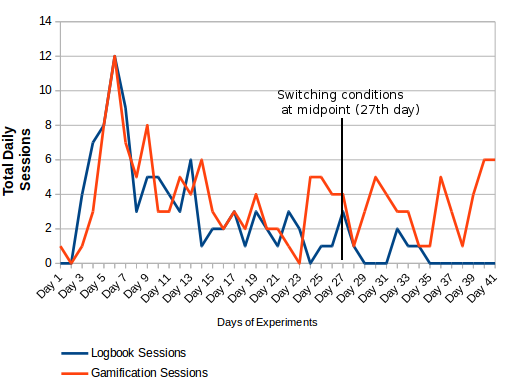
\includegraphics[width=0.6\textwidth]{Figures/scatter_daily_sessions.png}
    \rule{35em}{0.5pt}
  \caption{Comparison for trends of daily total sessions between logbook and gamification in 41 days of app usage.}
  \label{figure:usagedailysessions}
\end{figure}

\begin{table}[h!]
  \begin{center}
    \caption{Daily usage comparison between logbook and gamified systems for 41 days.}
    \label{table:usagedays}
	\begin{tabular}{|L{2.5cm}|c|c|c|c|c|c|}
		\hline
		Groups&N (days)&Mean&Sum Ranks&U&Z&P\\
		\hline
   		Daily logbook sessions&$41$&$33.72$&$1701.5$&\multirow{2}{*}{$1159.5$}&\multirow{2}{*}{$-2.9538$}& \multirow{2}{*}{$0.00318$}\\\cline{1-4} 
   		 		    Daily gamification sessions&$41$&$49.28$&$1701.5$&&&\\
\hline
	\end{tabular}
  \end{center}
\end{table}

\begin{figure}[htbp]
  \centering
    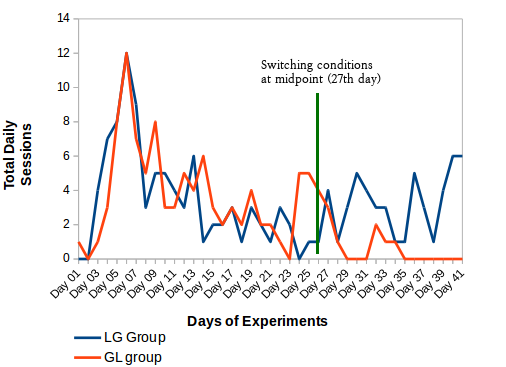
\includegraphics[width=0.6\textwidth]{Figures/usagedailysessions_lg_gl.png}
    \rule{35em}{0.5pt}
  \caption{Comparison of daily total sessions between LG group and GL group in 41 days of app usage.}
  \label{figure:usagedailysessions_lg_gl}
\end{figure}
\subsubsection{The Impact of Gamification Features on Internalization}\label{dim2}
An interesting phenomenon that expands on the usage pattern of Figure \ref{figure:usagedailysessions} is that of Figure \ref{figure:usagedailysessions_lg_gl}, which shows the usage trends of the LG (logbook-gamification) and GL (gamification-logbook) groups. It can be observed that there is a sudden drop in the number of usage sessions for users/pairs in the GL group after they switched from the gamification app to the logbook app. This pattern suggests that most behaviour regulation during the gamification condition was ego-involved (introjected) regulation. This hypothesized situation is supported by a further exploration of the number of impressions on gamification features. On checking the average impressions among the four gamification features, leaderboard had the highest average number of impressions, as shown in Figure \ref{figure:gamification_impressions_latest_all}. 
\begin{figure}[htbp]
  \centering
    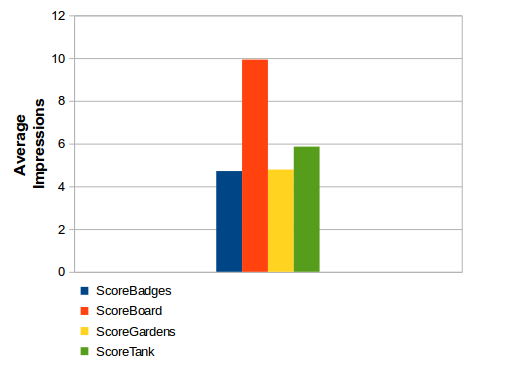
\includegraphics[width=0.6\textwidth]{Figures/gamification_impressions_latest_all.png}
    \rule{35em}{0.5pt}
  \caption{Total daily impressions for two groups (LG and GL).}
  \label{figure:gamification_impressions_latest_all}
\end{figure}
I conducted statistical comparisons on the number of impressions between leaderboard and each of the other gamification features (score badges, botanical garden and fish tank). The findings indicated that the number of impressions was significantly higher statistically for leaderboard ($Mean=9.93$, $SD=13.90$) than score badges ($Mean=4.71$, $SD = 5.50$) ($t (13) =2.1747$, $p=0.0487$). There was no statistical significance in either the number of impressions on leaderboard ($Mean=9.93$, $SD=13.90$) compared with botanical garden ($Mean = 4.79$, $SD = 5.26$) ($t(13)=1.716$, $p= 0.1096$) or the number of impressions on leaderboard ($Mean= 9.93$, $SD = 13.90$) compared with fish tank ($Mean=5.86$, $SD=7.40$) ($t(13)=1.5707$, $p = 0.1403$). However, the trend showed the dominance of leaderboard over other gamification features. 

A further exploration of gamification features' impressions revealed some insights on the trend of promotion of ego-involved and task-mastery climates. This exploration follows the discussion in the previous chapter (Chapter \ref{prototype2chapter}), where I observed that some statements from qualitative feedback reflected that gamification features tended to promote either a task-mastery climate or an ego-involved climate. In that discussion, the leaderboard tended to promote the ego-involved climate for some intermediary users, while features like the fish tank or botanical garden were inclined to promote the task-mastery climate. Literature suggests that the promotion of a task-mastery climate may foster integrated internalization of behaviour regulation, while the promotion of an ego-involved climate may only promote the introjected internalization of behaviour regulation~\citep{saksono2015spaceship}.

Since perceived usefulness is the only predictor of internalization (refer to the discussion on questionnaires in subsection \ref{methodsquestionnaire}), one of the logical steps was to compare perceived usefulness scores between intermediary users who had visited the leaderboard more often than other gamification features (i.e. the number of impressions on the leaderboard was greater than the number of impressions on any of the other gamification features) and those intermediary users whose number of impressions on the leaderboard was similar to or less than the number of impressions on any of the other gamification features. Since the average number of impressions on botanical garden, score badges and fish tank were fairly similar, as indicated in Figure \ref{figure:gamification_impressions_latest_all}, I selected only the botanical garden as a point of reference (to represent features that may promote a task-mastery climate) for comparison with leaderboard (to represent those features that may promote an ego-involved climate). 

Perceived usefulness concerned how intermediaries rated the usefulness of the app to them and their parents. I made an assumption based on literature that if the regulation was introjected, then the intermediaries would care less about the usefulness of the app. Therefore, the next task was to compare perceived usefulness between those intermediary users with high leaderboard impressions relative to the botanical garden and those with low leaderboard impressions relative to the botanical garden. In order to know whether an intermediary user fell into the high or low group, I computed a ratio by dividing the number of impressions on the leaderboard by the number of impressions on the botanical garden. After the computation of ratios, I divided 14 intermediary participants into two groups based on whether their ratio was below or above the median ($0.91$). As a result, I assigned seven intermediary users to a group with $ratio\geq Median$, while the remaining seven intermediary users were put into a group with $ratio<Median$. The next step compared perceived usefulness of the gamified app between intermediary users with $ratio \text{ of impressions }\geq Median$ and intermediary users with $ratio \text{ of  impressions }<~Median$. The two independent samples followed a normal distribution. Table \ref{table:pu_leaderboard_bias} shows the outcome  of a student-t test, which indicates that the group with $ratio<Median$ scored significantly higher in perceived usefulness than the group with $ratio\geq Median$. The implication of this finding is that those who had never accessed the leaderboard, or had accessed it fewer times relative to the botanical garden, had a higher tendency to view the intervention that utilized the gamified app as useful, compared to those who had used the leaderboard more than the botanical garden. 

\begin{table}[h!]
  \begin{center}
    \caption{Comparison of perceived usefulness between group with $ratio~\geq\textbf{Median}$ and group with ratio~\textless~\textbf{Median} (ratio = impressions on leaderboard/impressions on botanical garden).}
    \label{table:pu_leaderboard_bias}
	\begin{tabular}{|c|c|c|}
		\hline
		Mean &Group with ratio~\textgreater=~\textbf{Median}&Group with ratio~\textless~\textbf{Median}\\
		\hline
		 \multirow{2}{*}{Perceived usefulness}&$Mean=4.143$ ($SD = 0.763$)&$Mean=5.171$ ($SD = 0.962$)\\\cline{2-3} 

		 &\multicolumn{2}{|l|}{$t(12)=2.2156$, $p=0.0468$, 95\% $CI = -2.040 \text{ to }  -0.017$} \\
\hline
	\end{tabular}
  \end{center}
\end{table}

Since usage of leaderboard showed a significant decrease in scores of perceived usefulness, the next task was to see if that affected the gamification condition in general. Let's examine the trend of intermediaries' perceived usefulness between midpoint and endpoint for both the group with $ratio \geq Median$ and the group with $ratio \leq Median$. An earlier assumption was that the relationship between parents and children would make children view the app as meaningful; hence the regulation would be considered either identified or integrated regulation. But from the findings above, the trend indicated that most users concentrated on the leaderboard and, as a result, those with a higher number of impressions on the leaderboard than other gamification features such as the botanical garden had low scores in perceived usefulness.

In order to verify the significance of the aforementioned trend on impressions, I began with the hypothesis that gamification affected the perceived usefulness of the app through its leaderboard feature.  The first logical step was to assess perceived usefulness between midpoint and endpoint for the two aforementioned groups. The perceived usefulness was significantly higher at endpoint (Mean = 5.4, SD = 1.058) than midpoint ($Mean=4.67$, $SD=1.37$) ($t(6)=4.9670$, $p=0.0025$) for the group with $ratio<Median$, while for the group with $ratio>=Median$, there was no statistically significant difference between endpoint ($Mean=4.34$, $SD=1.081$) and midpoint ($Mean=4.66$, $SD=0.781$) ($t(6)=0.8742$, $p= 0.4156$). The intermediary user with the highest ratio was the one with the lowest scores on perceived usefulness. There was a negative correlation between ratio of impressions (leaderboard/botanical garden) and perceived usefulness without statistical significance ($r=0.52$, $p=0.06$, $N=14$).

What can be concluded so far from the trend on number of impressions is that it is very likely that the leaderboard played a role in hindering internalization, since perceived usefulness is a good predictor of internalization. High usage of leaderboard also suggests that most usage in gamification was, on account of ego-involved, introjected regulation.~The presence of introjected regulation is supported by the excerpt from one participant shown in Table \ref{table:introject_reg}, but it emerged in most of the excerpts of users while in the gamification condition. Therefore, usage in such cases was mostly influenced by the desire to dominate others in the competition. These different analyses support the conjecture of Figure \ref{figure:usagedailysessions} about the presence of introjected regulation due to a sudden drop in usage by pairs in the GL group  after day 27. If internalization was on the levels of identified and integrated regulations, then there would have been no sharp drop, but rather a steady one.  

\begin{table}[h!]
\renewcommand{\baselinestretch}{1.5}
  \begin{center}
    \caption{Excerpt: an example of introjected regulation.}
    \label{table:introject_reg}
	\begin{tabular}{|l|C{12cm}|}
		\hline
		No.&Comment\\
		\hline
		1.&\userquote{\textbf{Ayesha}, a beneficiary working with her son, 35 yrs} {``We [with Keagan] were not talking to others because all we wanted was to win. We didn't want them to know but they could see from the app.''}~\citep{katule2016family}\\
		\hline
	\end{tabular}
  \end{center}
\end{table} 

\subsubsection{Pairwise Comparison Between Logbook and Gamification}\label{dim3}
A different dimension of usage analysis looked at whether there was a significant difference in the number of sessions between the two experimental conditions (repeated measures of the same pairs in logbook and gamification conditions). As highlighted in the section above that describes the methods, the four pairs with technical glitches were excluded in order to make the comparison of the two experimental conditions fair (Table \ref{table:usageproblems}). The analysis showed that the means of logarithmic transformed data of normalized number of sessions between gamification and logbook were significantly different ($t(9)=2.6593$, $p=0.0261$)~\citep{katule2016family}. This implies that the number of times the app was used per day during the gamified condition was significantly higher than when pairs were in the logbook condition. The log mean had to be used in this comparison because the test for normality on differences of data points between logbook and gamification failed. A natural logarithmic transformation rectified the situation.

The next sub section report on user experiences of both intermediaries and beneficiaries.
\subsection{Intermediaries' User Experience}\label{interm_user_xp}
In most cases, the intermediary user facilitated usage of the app through proximate enabling and proximate translation. The work of~\cite{sambasivan2010} discussed these types of intermediated interactions. Baseline data indicated that intermediary participants had more interest in using cellphones than beneficiary participants. For instance, in an overall IMI scores to use a cellphone, intermediaries ($Mean=5.76$, $SD=0.41$, $N=14$) scored  significantly higher than beneficiary participants ($Mean=5.06$, $SD= 0.71$, $N=13$) with ($t(25)=3.1764$, $p=0.0039$).

If one refers back to the trend in Figure \ref{figure:usagedailysessions_lg_gl}, during the initial days of the experiment both gamification and logbook had patterns that were similar. However, after the second week, logbook usage started to go down while the trend for gamification remained steady for a couple of days. One of the possible explanations for why logbook had the same trend as gamification at the beginning is because both experimental conditions experienced the novelty effect which wore off after a few days. Also, the effect of having access to a smartphone contributed to high usage to most of the intermediary users in the logbook condition during phase 1 of the experiment. The act of sharing a phone during the intervention was important for nurturing the relationship between intermediaries and beneficiaries. In cases where parents shared the intervention's phone with their children, the children tended to be more interested in the intervention. Free access to the intervention's phone played a role in increasing the engagement of intermediary participants who did not have their own smartphones or data bundles in their smart-phones. In some cases, intermediary users installed and utilized other apps on the intervention's phones, such as games and social networks. To understand how the phone had a strong effect on motivation, I explored the relationship between perceived autonomy to use the cellphone at baseline and perceived enjoyment of using the Family Wellness app at midline for the group that started with the logbook. This exercise revealed an interesting phenomenon: there was a significant negative relationship between perceived autonomy to use a cellphone at baseline and perceived enjoyment of using the app at midline for the LG group ($r=-0.84$, $p=0.017$, $N=7$). A possible explanation for this is that those intermediary users with low autonomy to use a cellphone suddenly had free access to the intervention phone, and this increased their interest to participate in the intervention. For instance, one intermediary user (\textbf{Siphosethu}) from the LG group, who was the youngest participant (12 years of age), reported the lowest score in perceived autonomy to use a cellphone at baseline, and the highest score in  perceived enjoyment of using the app at midpoint (after using the logbook condition). She reported that she had freedom to use the intervention's phone as shown by the excerpt in Table \ref{table:interm_freed}.

\begin{table}[h!]
\renewcommand{\baselinestretch}{1.5}
  \begin{center}
    \caption{Excerpt: an example of a participant with freedom to use the intervention's phone.}
    \label{table:interm_freed}
	\begin{tabular}{|l|C{12cm}|}
		\hline
		No.&Comment\\
		\hline
		1.&\userquote{\textbf{Siyamthanda}, an intermediary} {``I had freedom because sometimes she left the phone with me and I was able to play games''}~\citep{katule2016family}\\
		\hline
	\end{tabular}
  \end{center}
\end{table}

There was an indication that having access to a phone, coupled with the novelty effect, had mediated engagement of some intermediaries that had started with the logbook condition. These intermediaries were helping their parents, and in return they had a free pass to access the intervention's cellphone. This finding is inconclusive due to the limited sample size; however, it highlights what could be explored in future studies. For the GL group it was difficult to isolate the gamification effect from the phone and novelty effect -- literature suggests that gamification has a novelty effect too~\citep{koivisto2014demographic}, for example. However, the trend shows that gamification accumulated more sessions compared to logbook, hence gamification alone increased utilization of the Family Wellness app. Gamification appeared to be the most dominant factor, that influenced usage, as we have already seen that the frequency of usage was higher in gamification than in logbook.

In addition to the novelty and phone effects, and gamification, another factor that contributed to intermediaries' interaction with the Family Wellness app was requests from beneficiaries. There were times when intermediary users opened the app for interaction only upon receiving requests from beneficiaries. In both absence and presence of gamification, intermediaries had to fulfil requests from beneficiaries.  But during the logbook condition, intermediaries appeared to be less enthusiastic in handling those requests. Some beneficiaries complained that there were several instances when their intermediary users refused to fulfil these requests, and this happened more often during the logbook condition. I had observed that in most of these cases, intermediary participants' autonomy was violated as requests came at times when intermediary participants were either studying for exams or doing something else, and they felt it was not the right time to fulfil those requests. As a result, some intermediary participants felt nagged by their parents. This happened during the logbook condition or in cases where gamification was demotivating for intermediary users who had not made progress~\citep{katule2016family}.

I categorized motivational drivers for all the requests that were put forward by beneficiary users to be originating from two main sources The first source of motivation was the instrumental value derived from using the app. The second source was gamification. Requests that were mediated by gamification fostered a sense of collaboration between members of a pair, while in the scenarios where beneficiaries were not concerned about gamification, or during the logbook condition, requests tended to be of an authoritative nature~\citep{katule2016family}. %Therefore the presence of gamification in this context tended to promote a collective responsibility for pairs where both members of a pair were motivated by gamification unlike in logbook condition where there was an absence of that cooperation.

\begin{table}[h!]
\renewcommand{\baselinestretch}{1.5}
  \begin{center}
    \caption{Excerpt: how gamification promoted collaboration.}
    \label{table:promote_collabo}
	\begin{tabular}{|l|C{12cm}|}
		\hline
		No.&Comment\\
		\hline
		1.&\userquote{\textbf{Ayesha}, a beneficiary}{``I would always ask him [Keagan] `Where are we. Are we first? And what badge do we have? Where are the others? How far is Simon [intermediary] then? How far is that one?' `No Mum, we are on top. We are first. We are the champions' [during gamification].''}~\citep{katule2016family} \\
		\hline
	\end{tabular}
  \end{center}
\end{table}

The excerpt from \textbf{Ayesha} (Table \ref{table:promote_collabo}) demonstrates a sense of collaboration between the two members of a participating pair (\emph{Ayesha} and \emph{Keagan}). The presence of gamification in this context tended to promote a collective responsibility for pairs (a sense of collectivism), where both members of a pair were motivated by gamification, unlike in the logbook condition where there was an absence of that cooperation. The excerpt shown in Table \ref{table:authoritarian} came from a beneficiary participant in the logbook condition and it indicated that she initiated usage while showing a sense of authority; it was not a cooperation between members of the pair. 

\begin{table}[h!]
\renewcommand{\baselinestretch}{1.5}
  \begin{center}
    \caption{Excerpt: a beneficiary demonstrating a tendency of being authoritative.}
    \label{table:authoritarian}
	\begin{tabular}{|l|C{12cm}|}
		\hline
		No.&Comment\\
		\hline
		1.&\userquote{\textbf{Sisipho}, a beneficiary working with her son, 43 yrs} {``I always start the conversation. Because I always want to make sure if he records because I can't use it. It was difficult for me to use it [during logbook].''}~\citep{katule2016family}\\
		\hline
	\end{tabular}
  \end{center}
\end{table}

The gamified app was designed in such a way that a pair would earn rewards based on cooperation between members: usage controlled by the intermediary participant and the average number of steps walked by the beneficiary participant (see more details in section \ref{prototype2descr}). The purpose of rewards was to foster users' intrinsic experiences such as competitiveness and a sense of autonomy, which are main contributors for intrinsic motivation, with the goal of improving collaboration between members of a pair. The presence of gamification nurtured teamwork even though the regulation of self-monitoring through intermediary users was mostly introjected (regulation done for the purpose of becoming better than others), as shown by the excerpts in Table \ref{table:introject_regulation2}.

\begin{table}[h!]
\renewcommand{\baselinestretch}{1.5}
  \begin{center}
    \caption{Excerpts: examples of teamwork as a result of competition from others.}
    \label{table:introject_regulation2}
	\begin{tabular}{|l|C{12cm}|}
		\hline
		No.&Comment\\
		\hline
		1.&\userquote{\textbf{Keagan}, an intermediary for his mother, 16 yrs} {``When I see other people trying to come above me [on the leaderboard], I hand over the phone to my mom so she can walk more steps.''}~\citep{katule2016family}\\
		\hline
		2.&\userquote{\textbf{Christine}, an intermediary for her mother, 16 yrs} {``I told my mom that me myself I want our team to have the highest points. `Yes', she said, she is going to do that.''}~\citep{katule2016family}\\
		\hline
	\end{tabular}
  \end{center}
\end{table}

Through these collaborations, goals were set. In most cases they were set by the intermediary user, who informed their beneficiary about what they wanted the team to do (excerpts in Table \ref{table:goal_formulation}); a pattern shown in Chapters \ref{prototype1chapter} and \ref{prototype2chapter} repeats itself for these intermediaries: a sense of joint ownership of the whole process in using the app. 

\begin{table}[h!]
\renewcommand{\baselinestretch}{1.5}
  \begin{center}
    \caption{Excerpts: examples of intermediaries suggesting goals for their team.}
    \label{table:goal_formulation}
	\begin{tabular}{|l|C{12cm}|}
		\hline
		No.&Comment\\
		\hline
		1.&\userquote{\textbf{Sophia}, an intermediary for her mother, 17 yrs} {``Sometimes that person may be first so I tell my mom that we must also be at the first place. [She looks at the  leaderboard and sees other people in the first place, and tells her mother that they should also aim for first position].''}\\
		\hline
		2.&\userquote{\textbf{Jenner}, a beneficiary working with her son, 45 yrs} {``When he [15-year-old Leon] looked through it [The app] and saw their points, he would say `Mom, we need to do something here, because look at their points and our points'. So it was quite interesting.''}\\
		\hline
	\end{tabular}
  \end{center}
\end{table}

Comparison of virtual rewards among intermediary users motivated them to check the app more often, compared with when they were in the logbook condition, as highlighted in the usage findings (subsection \ref{usageoutcome}). Intermediaries competed which each other through the leaderboard, and as a result there were frequent face-to-face interactions that entailed comparing scores, since most of the intermediary participants who lived in the same study's site (Langa or Athlone), either attended the same schools or lived not far from each other. The presence of these face-to-face interactions is shown an the excerpt in Table \ref{table:interm_facetoface}. These face-to-face interactions have been common throughout all evaluations reported in the previous chapters, as result in some situations, either the social features implemented in the app were never utilized or they were infrequent utilized. This part is revisited when presenting findings on relatedness, and it is further expanded in the discussion section, on its implications to the design of systems that encourage social comparison. 

\begin{table}[h!]
\renewcommand{\baselinestretch}{1.5}
  \begin{center}
    \caption{Excerpt: an example of face-to-face interactions between intermediaries.}
    \label{table:interm_facetoface}
	\begin{tabular}{|l|C{12cm}|}
		\hline
		No.&Comment\\
		\hline
		1.&\userquote{\textbf{Jenner}, a beneficiary} {``He [Leon] likes this exercise [using the app] because among him and his friends, they would have that competition like `I got more points than you' and that motivated him to get interested with the app.''}\\
		\hline
	\end{tabular}
  \end{center}
\end{table}
 
In most of the cases presented above, the pattern suggests that regulation was mostly introjected, as it was mediated by the need to be better than other participants in terms of points or being at the top of the leaderboard. This comparison among participants obscured the presence of other features to a great extent; this is proved by the fact that these features were not discussed in detail in the interviews, as intermediary users or beneficiary users who the researcher interviewed did not give any insights. The desire to be better than other participants led to cheating in some cases. For instance, in one pair, the beneficiary user and the intermediary user took turns to use the pedometer, therefore accumulating more steps and more points (Table \ref{table:cheating}). 

\begin{table}[h!]
\renewcommand{\baselinestretch}{1.5}
  \begin{center}
    \caption{Excerpt: an example of a case where steps were accumulated by both members of a pair.}
    \label{table:cheating}
	\begin{tabular}{|l|C{12cm}|}
		\hline
		No.&Comment\\
		\hline
		1.&\userquote{\textbf{Christine}, an intermediary for her mother, 16 yrs} {``I ask her `How far did you walk?' She would say she walked very far. She tells me that I must have the phone to walk more steps. She would say `I got more walking than you' [mother and daughter were collaborating in accumulating steps]. She sometimes writes the steps on the page and she tells me `Yesterday I had more points than you [points referring to steps]'.''} \\
		\hline
	\end{tabular}
  \end{center}
\end{table} 

Competition appeared to also affect pairs that had started with the logbook condition. Some intermediary users pushed their beneficiaries to do more, expecting rewards once they switched to the gamification condition. As a result, during the logbook condition there were intermediary participants who showed ambition to win while conversing with their respective beneficiaries~\citep{katule2016family}. The presence of gamification was also inclined to strengthen the family bond or relatedness between members of a participating pair (Table \ref{table:related_increase}).

\begin{table}[h!]
\renewcommand{\baselinestretch}{1.5}
  \begin{center}
    \caption{Excerpt: an example of an increase relatedness between members of a pair.}
    \label{table:related_increase}
	\begin{tabular}{|l|C{12cm}|}
		\hline
		No.&Comment\\
		\hline
		1.&\userquote{\textbf{Khanyiswa}, a beneficiary working with her daughter, 26 yrs} {``I think we talk more [with \textbf{Siphosethu}] than before the Family Wellness app. Before the Family Wellness app, after work it was just `Hi' and then I go to my room. But now she would come to my room  and say `Let me see your phone. What did you eat today?' and write everything down on the phone.''}\\
		\hline
	\end{tabular}
  \end{center}
\end{table} 

When it came to relatedness among intermediary users, social features were infrequent utilized: only two users showed interests towards such features. One of those two users appeared to attempt to make a social connection with other users through the app. It was observed that this particular user was not in physical contact with other users, hence using social features on the app was the only way to feel connected with others. One of the comments made by this user, to a fish tank that belonged to the other team is as shown in Table \ref{table:social_features}.

\begin{table}[h!]
\renewcommand{\baselinestretch}{1.5}
  \begin{center}
    \caption{Excerpt: an example of utilization for social features in the app.}
    \label{table:social_features}
	\begin{tabular}{|l|C{12cm}|}
		\hline
		No.&Comment\\
		\hline
		1.&\userquote{\textbf{Siphosethu}, an intermediary} {``Wow it shows that you are working hard  Clara\#2. [congratulating [Clara a female intermediary aged 14 years, for having her fish tank ranked number 2 in quality.]''}\\
		\hline
	\end{tabular}
  \end{center}
\end{table}    

The overall findings on user experience indicated mixed results, with some intermediary users having a positive experience while utilizing gamification, while the perceived enjoyment of some intermediary users was lower in gamification compared with logbook, despite the fact that there were more sessions reported in gamification. A leaderboard can indeed demotivate users at the bottom, but it can also foster aspects of relatedness for all users~\citep{sailer2013:psychological}. Since the leaderboard drew most attention, it could have played a role in demotivating users with lower performance. Therefore, in looking for evidence that supports this conjecture, I analysed the trend for both perceived enjoyment and usage, for each of the 14 intermediaries. As a result, I was able to identify several intermediary users whose trend for user experience showed a pattern worth discussing here. The process is as explained in the next paragraphs.

If we refer to the way the experiments were set, there were seven intermediaries in gamification, for each of the two phases of the experiment (phase 1: weeks 1\thinspace-\thinspace4, and phase 2: weeks 5 and 6). As a result, at any point of time, the leaderboard had seven teams. I went ahead to defining the criterion for identifying teams that were considered at the bottom, as the word bottom was vague. I looked for the teams that achieved only one badge (the lowest of all available badges) throughout the gamification condition; five teams in total were identified from both phases. Table \ref{table:bottom} shows the resulting list of teams at the bottom. The order of this list cannot be interpreted as pair's respective position on the leaderboard. Let's just view these teams as the bottom ones according to their respective leaderboard in either phase 1 or phase 2. The list also shows the total number of days that each team utilized the leaderboard and the change in the intermediaries' perceived enjoyment scores between gamification and logbook. A negative change means the score in gamification was lower than logbook, while a positive change means the score in gamification was higher than logbook. A negative change implies that, gamification harmed intrinsic motivation -- perceived enjoyment is the direct measure for intrinsic motivation. 

\begin{table}[h!]
  \begin{center}
    \caption{Pairs at the bottom of the leaderboard.}
    \label{table:bottom}
	\begin{tabular}{|c|c|c|c|c|c|}
		\hline
		&\multirow{2}{*}{Pair}&Intermediary's  & Group &Leaderboard's& Change in perceived\\
         &&pseudonym&sequence&visits (days) &enjoyment scores\\	
		\hline
		1&Pair-C&Lelethu&LG&0&1\\
		\hline
		2&Pair-D&Lindela&LG&2&-1.58\\
		\hline
		3&Pair-E&Leon&GL&4&-2.42\\
		\hline
		4&Pair-F&Keller&LG&4&-0.42\\
	\hline
		5&Pair-G&Jaquan&LG&1&0.25\\
	\hline
	\end{tabular}
  \end{center}
\end{table}

The findings in Table \ref{table:bottom} above, suggests that the negative change in motivation is observed in three intermediary users that accessed the leaderboard for at least two days. The simple explanation for the trend is that, users spent their first day of usage in trying to familiarise themselves with the gamification features. For those who came back to the leaderboard after the first day, it was because of the interest in comparing performance between them and others. Two users showed positive change: Lelethu (a 16-year-old male) and Jaquan (an 18-year-old female), but did not fully engage with the leaderboard (zero days for Lelethu and one day for Jaquan) like their peers at the bottom's list. Let's now answer the question for how the remaining three intermediaries, namely Keller (a 13-year-old male), Lindela (a 17-year-old male) and Leon, were negatively affected by the leaderboard. Let's start by reviewing Lindela's case first. Lindela's pair had their pedometer malfunctioned. The same situation happened to Lelethu, but unlike Lindela, his score on perceived enjoyment was higher in gamification than logbook. The two users had also shown more efforts in interacting with the logbook app before they switched to gamification; this is supported by a testimony from a 16-year old Anathi, who explained how unsure she was of the credibility of the gamified system, because her peers appeared to have more interest in the app but were at lower positions on the leaderboard than her (Table \ref{table:credibility}).

\begin{table}[h!]
\renewcommand{\baselinestretch}{1.5}
  \begin{center}
    \caption{Excerpt: an example of how technical glitches reduced the credibility of the app.}
    \label{table:credibility}
	\begin{tabular}{|l|C{12cm}|}
		\hline
		No.&Comment\\
		\hline
		1.&\userquote{\textbf{Anathi}, an intermediary for her mother} {``It [the experience of using the gamified app] was the same as last time [during the logbook condition] except for the game part. I was actually above some of the others. That was weird. Because they were more interested in the app than me. [She was making a reference to the two intermediary users that were found to be experiencing problems with their pedometers: Lindela and Lelethu. The three lived nearby each other''} \\
		\hline
	\end{tabular}
  \end{center}
\end{table}     

Anathi expected her peers to be more competent than her once she switched to gamification. Contrary to her expectations she was ahead of them, and this made her doubt her competence. This is further shown by her reported score on perceived competence in logbook and in gamification, where she reported lower score in gamification compared to logbook, despite using gamification for seven out of 14 days and logbook for only four out of 27 days. However, Anathi reported a slightly higher perceived enjoyment score  during gamification than logbook. This excerpt by Anathi together with the usage logs, suggest that an intermediary user from Pair-C (Lindela) was negatively affected with the leaderboard as a result of technical glitches. For Lelethu, his absence of contact with the leaderboard improved her perceived enjoyment in using the app while in the gamification condition. Also in this case, it is also clear that, technical glitches not only negatively affected the motivation of some intermediary users, but it also raised questions about credibility of the app. System credibility support has been highlighted as one the four important aspects of persuasive system design~\citep{Oinas-kukkonen:psd}. 

\begin{figure}[htbp]
  \centering
    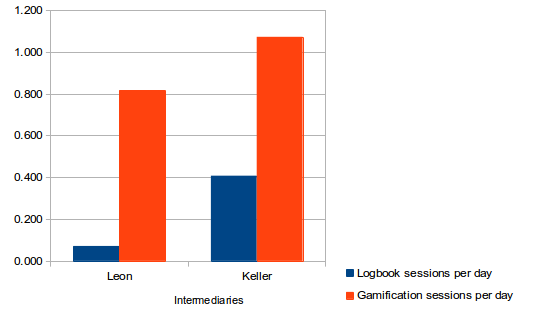
\includegraphics[width=0.5\textwidth]{Figures/badgesfailures2.png}
    \rule{35em}{0.5pt}
  \caption{Usage of two pairs with lack of progress in badges due to insufficient number of footsteps.}
  \label{figure:badge_failure_2}
\end{figure} 

The leaderboard also affected intermediary users in Pair-E and Pair-F (Leon and Keller), as a result of the app not being able to tailor challenges to the skills of the intermediary users. Their beneficiary participants were not walking enough steps, despite the fact that these two intermediaries had put more efforts into using the app during the gamification condition than in the logbook condition as shown in Figure \ref{figure:badge_failure_2} above; this means the two users were more eager to engage with the app in the gamification condition than logbook, but were let down by their beneficiaries. Their performance relied to a great extent on the performance of their respective beneficiary users. For the intermediary users in this case , their negative experience was assumed to be the result of the gamification design's failure to match challenges with abilities. The efforts of their beneficiary differed from their own, and this had an effect on the overall performance of the team. In that context, intermediary users had little control over the performance of their beneficiaries. Some intermediaries reacted negatively when they thought their beneficiary was not complying with carrying the pedometer when they should (Table \ref{table:negativereact}). 

\begin{table}[h!]
\renewcommand{\baselinestretch}{1.5}
  \begin{center}
    \caption{Excerpt: an example of negative reaction that threatened the social relationship between members of a pair.}
    \label{table:negativereact}
	\begin{tabular}{|l|C{12cm}|}
		\hline
		No.&Comment\\
		\hline
		1.&\userquote{\textbf{Jenner}, a beneficiary} {``Sometimes maybe I forget to take the phone when I go walking and he [Leon] would ask me `Did you take the phone with you?' `Ooh Gosh I forgot.'  Because when I walk to Park Town to exercise, sometimes  I am in such a hurry I forget the phone, and he gets crossed with me.''}\\
		\hline
	\end{tabular}
  \end{center}
\end{table} 

The excerpt above, demonstrates how an intermediary user was attempting to control his beneficiary user as a result of competition with intermediary users in other pairs. Instead of gamification being something enjoyable in this context it had a negative result that threatened the existing social rapport between parent and child. The exposure to the leaderboard contributed to the frustrating situation of not progressing. At one point, Leon contacted the researcher, because he wanted to know what else he needed to do in order to progress in the game. This suggests that challenges and skills were far apart.

In comparing the support of the three basic psychological needs in logbook and gamification, I made a decision to exclude four intermediary users, whose perceived enjoyment was largely affected by either technical glitches or exposure to the leaderboard coupled with the inability to participate fairly in gamification because of either the pedometer not working or design limitations of the app. The first three intermediaries have already been discussed above: Lindela (Pair-D), Pair-E (Leon) and Keller (Pair-F). The fourth intermediary user on the list is from Pair-A in Table \ref{table:usageproblems}. The technical glitches negatively affected his whole user experience of using the app and this happened during the gamification condition. His experience is reflected by the message in Table \ref{table:negativexp} that he sent to the researcher. The message was sent on the 11\SP{th} day since the beginning of the experiment, through the chat room that was available on the app. 

\begin{table}[h!]
\renewcommand{\baselinestretch}{1.5}
  \begin{center}
    \caption{Excerpt: an example of negative user experience due to technical glitches.}
    \label{table:negativexp}
	\begin{tabular}{|l|C{12cm}|}
		\hline
		No.&Comment\\
		\hline
		1.&\userquote{\textbf{Nathan}, an intermediary for his father, 20 yrs} {``Chief! [Chief -- a nickname for the researcher] This app is unstable. Kicks me out for days, stops running, doesn't respond, exits when orientation changes and the list goes on. As for the pedometer, that too has bugs. It crashes or sometimes freezes (doesn't respond), makes it difficult to use the app.''}\\
		\hline
	\end{tabular}
  \end{center}
\end{table}    

The decision to exclude the four pairs above, aimed to minimize the negative effect of extraneous factors in reducing the power of the study, in detecting differences in motivation scores between the logbook condition and the gamification condition. These extraneous factors were: weak design  for gamification -- as the system lacked the ability in supporting adaption of challenges to skills, and the unexpected technical problems that affected the overall user experience. 

As a result of excluding the scores of four intermediary participants, only 10 out of 14 intermediary users were considered in the subscales that measured the three aspects of SDT (autonomy, competence and relatedness). On perceived competence in using the app, the gamified condition scored significantly higher than the logbook condition ($t(9)=3.495$, $p=0.0068$)~\citep{katule2016family}. There was no significant difference between logbook and gamification scores of perceived autonomy ($t(9)=0.027$, $p=0.98$) and perceived relatedness ($t(9)=0.719$, $p=0.49$)~\citep{katule2016family}.

\subsection{Beneficiaries' User Experience}\label{ben_user_xp}
As most beneficiaries only interfaced with the app through intermediary users, beneficiaries' user experience relied on cooperation from intermediaries. Concerning support for the three basic psychological needs, there was no difference between logbook and gamification. However, relatedness ($N=14$) appeared to improve significantly with time between midpoint ($Mean=4.43$, $SD=0.92$) and endpoint ($Mean=5.38$, $SD=1.08$)($t(13)=2.3736$, $p=0.0337$). Therefore, the intervention in general made beneficiaries feel more related to others (their respective intermediaries and other beneficiaries) who were part of the intervention.
  
When utilizing the app through intermediaries, there were cases where beneficiaries had a negative experience as a result of intermediaries refusing to assist when asked to. This happened in cases where intermediary users did not feel like helping, either because they were occupied by other tasks such as learning for exams, or because they felt the app was boring, especially in the logbook condition. 

In the next subsection, the IMIs in the self-monitoring of diet and activity are reported on. Four pairs with usage problems (Table \ref{table:usageproblems}) were excluded due to their self-monitoring being affected. Therefore, in total only 10 out of 14 beneficiaries had their results included for analysis, in order to have only beneficiaries who had meaningful engagement with the app through their respective intermediaries.
\subsubsection{IMI in Self-Monitoring of Diet}
The results for self-monitoring of diet (baseline, midline and endline) are shown in Table  \ref{table:imidietbenf}. The Mauchly’s test indicated that the assumption of sphericity was not violated with  $\chi{}^2(2)=3.76$, $p=0.152$. The results ($N=10$) on self-monitoring of diet shown in Table \ref{table:imidietbenf}, were from sphericity assumed output. ANOVA showed that there was a significant difference in average IMI scores for self-monitoring of diet measured at baseline, midline and endline.
\begin{table}[h!]
  \begin{center}
    \caption{Comparison of 10 beneficiaries' IMI scores in self-monitoring of diet at baseline, midline and endline.}
    \label{table:imidietbenf}
	\begin{tabular}{|L{2.8cm}|L{3.2cm}|L{3.2cm}|L{3.2cm}|}
		\hline
		Mean IMI Score &Baseline&Midline&Endline\\
		\hline
		 %\multirow{3}{*}
		 {Self-monitoring}&$Mean=4.48$, $SD=1.24$&$Mean=5.07$, $SD=1.19$&$Mean=5.55$, $S.D=0.95$\\\cline{2-4} 

		of Diet &\multicolumn{3}{|l|}{$F(2,18)=3.787$, $p=0.042$} \\
\hline	\end{tabular}
  \end{center}
\end{table}
A finding from pairwise comparisons (a paired student t-test) indicated that the IMI score at endline was significantly higher than at baseline (Table \ref{table:imipairwisediet}). The difference between baseline, midline and endline was not significant (Tables \ref{table:imipairwisediet1}, and \ref{table:imipairwisediet2}). Motivation to self-monitor diet appeared to increase with time, as shown in Figure \ref{figure:imi_diet}. The interpretation of the above findings is that the wellness app appears to have had a significant effect over time on the motivation of beneficiaries to self-monitor their diet.
\begin{table}[h!]
  \begin{center}
    \caption{Pairwise comparisons of IMI scores for self-monitoring of diet: baseline versus midline.}
    \label{table:imipairwisediet}
	\begin{tabular}{|L{2cm}|L{4cm}|L{4cm}|}
		\hline
		Mean &Baseline&Midline\\
		\hline
		 \multirow{2}{*}{IMI Score}&$Mean=4.48$, $SD=1.24$&$Mean=5.07$, $SD=1.19$\\\cline{2-3} 

		 &\multicolumn{2}{|l|}{$t(9)=1.298$, $p=0.227$} \\
\hline
	\end{tabular}
  \end{center}
\end{table}
\begin{table}[h!]
  \begin{center}
    \caption{Pairwise comparisons of IMI scores for self-monitoring of diet: baseline versus endline.}
    \label{table:imipairwisediet1}
	\begin{tabular}{|L{2cm}|L{4cm}|L{4cm}|}
		\hline
		Mean &Baseline&Endline\\
		\hline
		 \multirow{2}{*}{IMI Score}&$Mean = 4.48$, $SD = 1.24$&$Mean = 5.55$, $SD = 0.95$\\\cline{2-3} 

		 &\multicolumn{2}{|l|}{$t(9)=2.457$, $p=0.036$} \\
\hline
	\end{tabular}
  \end{center}
\end{table}
\begin{table}[h!]
  \begin{center}
    \caption{Pairwise comparisons of IMI scores for self-monitoring of diet: midline versus endline.}
    \label{table:imipairwisediet2}
	\begin{tabular}{|L{2cm}|L{4cm}|L{4cm}|}
		\hline
		Mean &Midline&Endline\\
		\hline
		 \multirow{2}{*}{IMI Score}&$Mean=5.07$, $SD=1.19$&$Mean=5.55$, $SD=0.95$\\\cline{2-3} 

		 &\multicolumn{2}{|l|}{$t(9)=1.975$, $p=0.08$} \\
\hline
	\end{tabular}
  \end{center}
\end{table}

\begin{figure}[htbp]
  \centering
    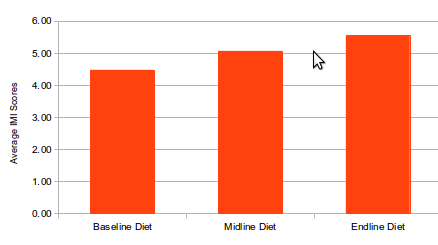
\includegraphics[width=0.4\textwidth]{Figures/imi_diet.png}
    \rule{35em}{0.5pt}
  \caption{Trend for average IMI scores for self-monitoring of diet at three points: baseline, midline and endline.}
  \label{figure:imi_diet}
\end{figure}
This ANOVA finding does not discern between the different experimental conditions which pairs of users were exposed to. The ANOVA finding (N=10) (Table  \ref{table:imidietbenf2}) on the comparison of IMI scores for the self-monitoring of diet during baseline, logbook, and gamification conditions showed that there was no significant difference in average IMI scores. This finding was a result of sphericity-assumed output of the ANOVA test, since the Mauchly’s test indicated that the assumption of sphericity was not violated with  $\chi{}^2(2)=2.19$, $p=0.335$. The trend for averages shows both logbook and gamification to be slightly higher than baseline, as shown in Figure \ref{figure:imi_diet2}. The conclusion from this finding is that both versions of the prototype cause an increase in motivation of beneficiaries to self-monitor their diet.
\begin{table}[h!]
  \begin{center}
    \caption{Comparison of 10 beneficiaries' IMI scores for self-monitoring of diet at baseline, after logbook, and  after gamification conditions.}
    \label{table:imidietbenf2}
	\begin{tabular}{|L{2.8cm}|L{2.5cm}|L{2.5cm}|L{2.5cm}|}
		\hline
		Mean IMI Score &Baseline&Logbook&Gamification\\
		\hline
		 %\multirow{3}{*}
		 Self-monitoring&$Mean=4.48$, $SD=1.241$&$Mean=5.28$, $SD = 1.05$&$Mean=5.34$, $SD=1.16$\\\cline{2-4} 
		 of Diet&\multicolumn{3}{|l|}{$F(2,18)=3.787$, $p=0.087$} \\
\hline	\end{tabular}
  \end{center}
\end{table}
\begin{figure}[htbp]
  \centering
    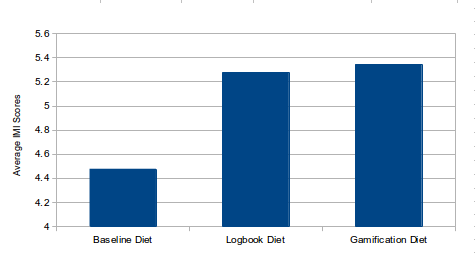
\includegraphics[width=0.4\textwidth]{Figures/imi_diet2.png}
    \rule{35em}{0.5pt}
  \caption{Trend for average IMI scores for self-monitoring of diet at three points: baseline, logbook and gamification.}
  \label{figure:imi_diet2}
\end{figure}
\subsubsection{IMI in Self-Monitoring of Activity}
The results for self-monitoring of activity are shown in Table  \ref{table:imiactivitybenf}. The results are based on a sample of nine beneficiary users, as one participant did not complete this part of the questionnaire at baseline.  The Mauchly’s test indicated that the assumption of sphericity was violated with  $\chi{}^2(2)=8.248$, $p=0.016$. The value $\epsilon$ on Greenhouse-Geisser was $<0.75$, therefore, I selected the results for self-monitoring of activity shown in Table \ref{table:imiactivitybenf} from Greenhouse-Geisser output. ANOVA showed that there was no significant difference in the average IMI scores for self-monitoring of activity measured at baseline, midline and endline. The trend of means increases from baseline to endline, as shown in Figure \ref{figure:imi_activity}.

There are several factors that might have contributed to results not being significant among baseline, midline and endline points. The first hypothesized reason is that tracking of physical activity appeared to be easy for the majority of the participants, even without tracking devices, as people can estimate the distance they walk daily and they consider this to be tracking, even though they might not have means to record this information. Hence participants' motivation was high at baseline, unlike diet self-monitoring, which they considered to be cumbersome due to external barriers such as healthy food being expensive and lacking of knowledge about healthy food; therefore at baseline, participants felt more motivated to track their activity. The second hypothesized reason is that the sample size was small, hence it was more difficult to detect a significant difference. But we have seen that the trend in motivation increases with time.
\begin{table}[h!]
  \begin{center}
    \caption{Comparison of 10 beneficiaries' IMI scores for self-monitoring of activity at baseline, midline and endline.}
    \label{table:imiactivitybenf}
	\begin{tabular}{|L{2.8cm}|L{2.5cm}|L{2.5cm}|L{2.5cm}|}
		\hline
		Mean IMI Score &Baseline&Midline&Endline\\
		\hline
		 %\multirow{3}{*}
		 Self-monitoring&$Mean=4.82$, $SD=1.002$&$Mean=5.28$, $SD=1.003$&$Mean=5.41$,$SD=0.894$\\\cline{2-4} 
		 of activity&\multicolumn{3}{|l|}{$F(1.182, 9.455)=2.936$, $p = 0.116$} \\
\hline	\end{tabular}
  \end{center}
\end{table}

\begin{figure}[htbp]
  \centering
    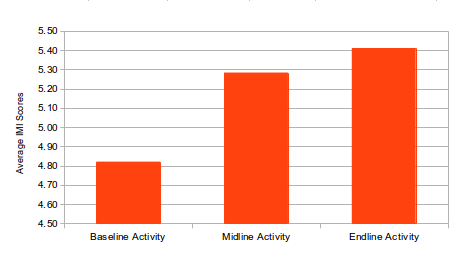
\includegraphics[width=0.4\textwidth]{Figures/imi_activity.png}
    \rule{35em}{0.5pt}
  \caption{Trend for average IMI scores for self-monitoring of activity at three points: baseline, logbook and gamification.}
  \label{figure:imi_activity}
\end{figure}
The finding from an analysis ($N=9$) where I examined if there was a difference between baseline, logbook and gamification in self-monitoring of activity, showed that there was no significant difference of average IMI scores (Table \ref{table:imiactivity2benf}). The Mauchly’s test indicated that the assumption of sphericity was violated with  $\chi{}^2(2)=6.788$, $p=0.034$. The value of $\epsilon$ on Greenhouse-Geisser was \textless 0.75; therefore, I selected the results for  self-monitoring of activity from Greenhouse-Geisser output of one-way ANOVA (with repeated measures) test. The trend in motivation increases in both logbook and gamification compared to baseline, as shown in Figure \ref{figure:imi_activity2}
%epsilon=0.617
\begin{table}[h!]
  \begin{center}
    \caption{Comparison of 10 beneficiaries' IMI scores for self-monitoring of activity at baseline, logbook and gamification.}
    \label{table:imiactivity2benf}
	\begin{tabular}{|L{2.8cm}|L{2.5cm}|L{2.5cm}|L{2.5cm}|}
		\hline
		Mean IMI Score &Baseline&Logbook&Gamification\\
		\hline
		 %\multirow{3}{*}
		 Self-monitoring&$Mean=4.82$, $SD=1.002$&$Mean=5.33$, $SD=0.9762$&$Mean=5.37$,$SD=0.9276$\\\cline{2-4} 
		 of activity&\multicolumn{3}{|l|}{$F(1.234, 9.872)=2.783$, $p=0.123$} \\
\hline	\end{tabular}
  \end{center}
\end{table}
\begin{figure}[htbp]
  \centering
    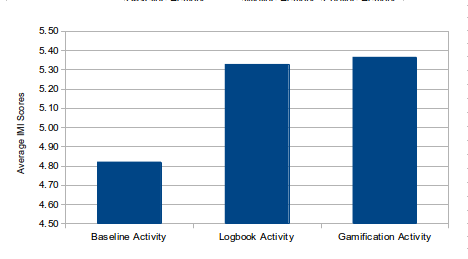
\includegraphics[width=0.4\textwidth]{Figures/imi_activity2.png}
    \rule{35em}{0.5pt}
  \caption{Trend for average IMI scores for self-monitoring of activity at three points: baseline, logbook and gamification.}
  \label{figure:imi_activity2}
\end{figure}

\section{Discussion}
\subsection{Motivational Affordances' Impact on Intermediaries}
As reported above, intermediary users facilitated interaction with the app. Intermediaries were motivated to engage with the app mostly because of two main reasons: either to follow up on competition with others, or in response to requests from their respective beneficiary users. Gamification was the main source of motivation for intermediaries. It played a pivotal role in mediating usage during the gamification condition, and even in the logbook condition for intermediary users in pairs that had started with the logbook condition before being switched to gamification. Some users who started with the logbook condition were eager to experience gamification, and this motivated them to sustain engagement while in logbook. This was true in the case of \textbf{Siphosethu}, an intermediary user who talked of winning while still in logbook condition. This affected the separation of experimental conditions, since the randomization of experimental sequences was not blind. Those that started with logbook already knew that they would start using gamification after a period of three weeks, and this positively affected their engagement with the app. On perceived competence, the difference between logbook and gamification was statistically significant, showing intermediary users in gamification felt more competent. A statistically significance difference was not seen for autonomy and relatedness, possibly due to uncontrolled interaction between experimental conditions and some other contextual factors that I have hypothesized later on this section. Perceived competence and perceived autonomy are the most important predictors of intrinsic motivation. 

From the findings it is also evident that gamification played a role in improving intermediaries' perceived enjoyment (a direct measure of intrinsic motivation) in using the app, except for a few cases where it appeared to harm  perceived enjoyment due to several reasons already highlighted in the findings section above. For instance, the use of leaderboard had both positive and negative effects depending on the characteristics of the intermediary user and pair in general. Intermediary users responded differently to gamification due to great variation in users' traits (personalities) and the skills possessed by their respective team mates (beneficiaries), leading to mixed results. Literature has vastly explored how important it is to tailor game design mechanics to players' personalities. One survey that investigated how preferences in motivational affordances are linked to individuals' personality traits came to the following conclusions: (1) extraverts tend to be motivated by points, levels and leaderboards; (2) avatars are likely to be preferred by people with high levels of imagination; (3) extraverts prefer to be centre stage; hence the position they desire in a feature like a leaderboard is the top one; and (4) introverts may not be comfortable in a crowd of strangers~\citep{jia2016personality}. Personality traits that are exhibited by game players may also cross over into gamification, since the boundary between gamification and games is diminishing~\citep{ferro2013towards}. What may be considered a simple gamified system in one context will be socially perceived as a game in a different context~\citep{deterding2011game}. Personalization of healthy interventions for gamer types  is already common~\citep{arteaga2010:persuasive,orji2013:tailoring}, but it has only been used in the context of direct users of technology and not in the context of intermediary and beneficiary users.

Apart from tailoring game mechanics, another aspect of personalization is  the tendency of involuntary participation in gamification features. Involuntary participation might violate users' autonomy. Gamification borrows its game mechanics from games, and playing games has been pointed out as voluntary~\citep{seaborn2015:gamification,knaving2013designing}. Participating in a gamification layer should be opt-in (invisible) and not mandatory, in order not to obscure the main activity being promoted~\citep{knaving2013designing}. In most current gamification designs, the line between voluntary and involuntary participation is not clear, as a user may voluntarily participate in gamification but involuntarily participate in a feature like a leaderboard, which may come as part of the package of gamification~\citep{ferro2013towards}. This concerns the autonomy of users in selecting which parts of gamification they would like to participate in. There was an additional aspect of autonomy that was a shortcoming in this intervention, and that was the inability of intermediary users to select the level of gamification appropriate for their skills. The only support for autonomy that the app provided was the configuration of avatars and editing of team profiles. Intermediaries stated goals, as indicated in the findings, but were not able to accomplish them as the goals largely depended on the skills of their respective beneficiaries. Literature suggests approaches on which autonomy could be supported; these include, but are not limited to, configuration of profiles, avatars, macros, configurable interface, alternative activities and privacy control~\citep{francisco2012analysis}. These approaches may scale to the context of technology use through intermediaries, but there is a need to explore how intermediary users can have autonomy in the formulation and execution of goals to tackle challenges based on their skills. When challenges are too difficult, because they do not match users' skills, end users can become demotivated \citep{zhang2008motivational}.    

Absence of autonomy in the formulation and execution of goals may foster  negative experiences, which appeared to harm the intrinsic motivation of some intermediary users in this context. For instance, in most cases the presence of gamification fostered collaboration between intermediary and beneficiary members of a pair. Out of this collaboration, intermediaries attempted to influence or persuade their respective beneficiaries. Negative experiences ensued when persuasion did not work or there was evidence of non-compliance by beneficiaries. An example of a negative experience is when nudging evolves into nagging, like in the case of \textbf{Jenner} above. A beneficiary user, she described how seriously her son was taking the competition with others by constantly reminding her to carry the pedometer whenever she wanted to go out, and at times her son would get annoyed if she forgot to carry the pedometer. The ramification of this is that it deviates from the goal of promoting collaboration between an intermediary user and a beneficiary user, and instead creates tension between them. In such scenarios, intermediary users may react out of frustration of not having control of the skills possessed by their respective beneficiaries. Intermediaries relying solely on the skills of their respective beneficiaries did  not help the effort to match challenges with user skills, and it was the main source of tension between members of a pair. 

An approach that could be used to minimize the effect of the  aforementioned shortcoming is to give users more autonomy to select different levels of gamification. There could be levels such as beginner, intermediate and advanced. Pairs that are on the same level could be grouped together and not mixed with pairs on different levels. In addition, users could be allowed to select which features they would like to include in their interfaces from a range of features such as chatrooms, leaderboards and botanical gardens. More autonomy could also be given through the customization of privacy, in terms of whether or not participants would like to share their information. Customization of avatars is also important; it was observed that most users changed their avatars during gamification, and one user explained that she saw the avatar she selected as a representation of herself. These avatars embodied intermediary users' identities.

The second possible approach for increasing the engagement of intermediary users is to give intermediary participants a direct benefit, by incorporating their own wellness data (i.e. steps). There were some observed scenarios that support the utilization of this approach. For instance, there was one pair in which both the beneficiary and intermediary participants were using the pedometer. They took turns to use it, thus collaborating in accumulating steps, and had discussions of whether the person whose turn it was had walked enough steps. The goal was to accumulate more steps than other pairs. A similar concept has been explored with participants in a low-income neighbourhood in the USA, using an exergame that encourages cooperation between parents and children~\citep{saksono2015spaceship}. This approach of supporting direct participation of intermediary users can also be combined with the customization approach we discussed above.

A third proposed way of increasing engagement takes into account the intermediaries' claims that also they benefited from nutrition/diet information, since the same type of meal is shared at home. If beneficiary participants ate something unhealthy while at home, then it was likely the intermediary participant would it too.~According to literature, parents who live a healthy lifestyle are likely to influence their children to live healthily~\citep{grimes2009toward}. It is possible that by creating a system that allows intermediaries to also benefit from usage, one can foster regulation that is either type \emph{identified} or type \emph{integrated}, which are both nearer to the border that separates extrinsic motivation from intrinsic motivation. 

Apart from gamification, another important source of motivation which one could leverage is the sharing of phones between participating members of a pair. Beneficiaries were custodians of intervention's phone, but in many cases, when beneficiaries were at home, they left the phone with the intermediaries who were interested in social media sites and games. Intermediaries were interested in the phones for both or either of these two reasons: (1) the intervention's phones were better than the intermediaries, or intermediaries did not have smartphones that could access services they desired; and (2) the free data bundles on the intervention's phones (data provided by the research at the beginning). In these scenarios, some intermediaries were implicitly reciprocating the favour of having freedom to use the phone with responding to requests from their beneficiaries. This kind of non-prescribed use is important and it has the capability to increase engagement of participants in an ICTD intervention~\citep{ferrplay2015}. One can capitalize on this motivation, introduced as a result of sharing phones, and it can be viewed as part of motivational affordances to encourage the ongoing use of a system through young intermediaries within family settings. Utilization of the motivational effect of the phone in mediating such an intervention depends on the interest of beneficiaries in the intervention. Without requests from beneficiaries, and with the absence of gamification on the app for intermediaries, the phone effect itself cannot mediate usage of the app, unless it works in tandem with those two mediating factors.

Perceived relatedness is the last aspect of self-determination theory worth discussing. The trend of intermediary users not using social features recurred from the previous chapters. There were face-to-face interactions outside the context of usage logs, as can be noted from some of the participants' excerpts. These interactions crossed over beyond the boundaries of the experimental conditions (logbook and gamification). As has been highlighted in the study by~\cite{lin2006:fish}, social features may be appropriate in contexts where users are not in close proximity; hence there is absence of face-to-face interactions and the only way for users to interact is through social features provided by the app. For instance, the one intermediary user was keen to use the social features did not have face-to-face interactions with the rest, besides at the meeting organized by the research team. 
\subsection{Motivational Affordances' Impact on Beneficiaries}
As was reported on in the findings section, beneficiaries engaged with the app through intermediaries upon either the intermediaries coming to them or the beneficiaries requesting that something be done on the app. Requests from beneficiaries were as a result of their being interested in either the leaderboard, the instrumental value provided by the app or both. Not all beneficiaries were motivated by gamification. Different strategies are required in order to engage older adults. Literature suggests that emotional stability increases with age~\citep{carstensen2011emotional}; this implies that adults tend to have higher emotional stability than children. Gamification may be less effective for people with higher emotional stability~\citep{jia2016personality}. In the previous chapter (Chapter \ref{prototype2chapter}), I as the researcher observed that adults cared most about social support from other adults, and social comparison increased their perceived relatedness. In this evaluation, there were fewer interactions between beneficiaries, hence less social comparison among beneficiaries alone. Improving the relatedness of beneficiaries may be one way to improve their engagement. Also, features that promote a task-mastery climate may be of interest to this group of participants. For instance, one intermediary participant reported that her mother was more interested in the botanical garden than her. 

In general, the app was perceived well by beneficiaries, and gamification was of less importance compared with the perceived value of the app. This was demonstrated by the overall scores of intrinsic motivation inventory (IMI) for the self-monitoring of diet and activity. The improvement in the IMI score from baseline to endpoint for the self-monitoring of diet was significant, while for the self-monitoring of activity there was an indication of improvement but without statistical significance.
\subsection{Internalization of Helping in Self-Monitoring}
The dominance of the leaderboard resulted in introjected regulation mostly where individuals do not view a behaviour as  having value in itself; rather individuals perform that behaviour for the sake of maintaining their self-worth. This had an impact on internalization. Those intermediary users that had no contact with the leaderboard, or fewer contact than other gamification features, reported viewing the intervention as more useful in gamification than logbook condition. It is clear that the leaderboard had a tendency to create an atmosphere of introjected regulation, and this kind of regulation overshadowed the main activity (monitoring the health of beneficiary users). A challenging task is to design gamification in such a way that it does not become the main focus, taking away from the activity being promoted~\citep{knaving2013designing}.

A leaderboard may be appropriate for some users, but it has a negative effect on others -- this has already been highlighted in the discussion about personality traits and gamer types, and perceived autonomy. This finding cannot be conclusive as it stands due a sample size I used, but it can be the basis for a much larger study with a bigger sample size, in order to test the hypothesis about the domination of introjected regulation in the presence of a leaderboard.

\subsection{Impact of Cognitive Flow on User Experience}
One important aspect in supporting optimal cognitive flow is to provide feedback on time~\citep{csikszentmihalyiflow}. Flow has been examined in the context of direct usage, not in intermediated use. Therefore, exploring maintenance of flow in the context of intermediated use is crucial for improving the user experience. One of the challenges in the intervention was achieving an optimal flow in intermediated use. I had installed the application on one phone to be shared by a pair and beneficiary users were the ones that had custody of the phone. Therefore, in most cases intermediaries only had access to the phone when around their beneficiary. Although this arrangement proved to be beneficial in collaborative reflection, but it resulted to challenges of not having timely feedback in some cases where the beneficiary user was away -- intermediaries had limited access to the app since their respective beneficiaries had gone away with the phone. In those situations, beneficiaries did not have someone to help them translate their intents into the app, while at the same time, intermediaries did not have physical means to translate their intents into the app. This had a negative impact on the cognitive flow of both sets of users, as they could not self-reflect on time. This raises the question of how to optimally maintain flow. How users and technology are arranged, can have an impact on cognitive flow; intermediaries need to be able to access a system, even in cases where their respective beneficiary users are not present. On the side beneficiaries, services that are easy to access such as SMS can be used to give timely feedback.

\section{Chapter's Contribution}
The contribution of this chapter is on understanding the role of gamification in increasing collaboration between an intermediary user and a beneficiary user. I have discussed how gamification can be effective in fostering or preventing internalization. The leaderboard was the main source of introjected regulation here; hence it prevented optimal internalization of helping in self-monitoring tasks. Generally, gamification appeared to increase collaboration between members of a pair. This collaboration seemed to strengthen bonds, which is crucial for future negotiations of interaction between an intermediary user and beneficiary user. However, in some scenarios, where competition through the leaderboard was excessive, gamification created tension that threatened the relationship between an intermediary user and a beneficiary user. This happened in cases where an intermediary user felt the non-compliant behaviour (e.g. forgetting to carry the phone running the pedometer) of their beneficiary user was letting down the team.  This also brings in the concept of personality types, and the importance of matching them with gamification features that support them.

In this chapter, it also became clear how a confounding factor such as sharing phones can play a role in increasing collaboration. I argued that such confounding variables should not be viewed as affecting the rigour of a study, but as contextual facilitators of an intervention. However, since the experiment design was within-group, such confounding factors affected the same intermediary users in both experimental conditions; hence they did not affect any comparison between logbook and gamification.~Designers of collaborative systems such as the one in this study need to take all the discussed factors into consideration in order to design a system that is emotionally engaging in a positive way. This chapter has brought to light both the pros and cons of gamification in the context of intermediated use. The next chapter reflects back to the research questions and provides a general view of the contribution and limitations, of this thesis.
\begin{flushright}
\end{flushright}


% Chapter 1

\chapter{Conclusions and Future Research} % Main chapter title

\label{discussionchapter} % For referencing the chapter elsewhere, use \ref{Chapter1} 

\lhead{Chapter \ref{discussionchapter}. \emph{Conclusions and Future Research}} % This is for the header on each page - perhaps a shortened title

%----------------------------------------------------------------------------------------
The main research questions were centred around the factors that could affect utilization of a personal health informatics application through intermediaries, and also the effectiveness of gamification in increasing both engagement of intermediaries and collaboration between members of a pair in intermediated use. This chapter revisits the research questions and discusses how they were addressed. It also summarizes takeaways which can be regarded as design considerations for motivational affordances in intermediated use of a self-monitoring application that promotes healthy behaviours. These design considerations reveal social factors that can contribute to the success of an intervention such as the one in this study, and motivational strategies that can be utilized to keep both intermediaries and beneficiaries engaged with a personal health informatics (self-monitoring) system/application.

\section{Discussion of Research Questions}
The main focus of this research was to uncover how social factors and persuasive systems' inspired motivational affordances might impact intermediated use of personal health self-monitoring applications. Intermediated technology use is an interaction model that is prevalent in low-income areas of the developing world. Many health self-monitoring applications have motivational affordances that cater for personal or direct usage, but such motivational affordances have not been explored in the context of intermediated use. In order to understand design requirements for motivational affordances targeting intermediated use, this research aimed to provide answers to the following research questions.

\textbf{RQ1}: What is the role of social-technical settings in the intermediated use of a gamified self-monitoring application targeting the promotion of healthy eating and physical activity? 

This research question had two sub-questions. The first aimed to identify prerequisite factors that could affect intermediated use, and the second explored the extent to which an understanding of the identified factors is important in the context of intermediated use. In order to provide answers to these research sub-questions, I conducted a series of studies. These studies included one contextual enquiry (Chapter \ref{contextualenqchapter}) and two consecutive evaluations of two versions of the prototype (Chapters \ref{prototype1chapter} and \ref{prototype2chapter}). 

The most noteworthy factors that came to light in the aforementioned studies included but were not limited to, social relationship; collaborative reflection using a shared device; and motivational affordances, either as part of the app or socially constructed as a result of using the app. 

Informative evaluations suggested that involving children who are family members is the key to the success of this kind of intervention, and running an app running on a shared device increases the tendency of members of a pair to reflect collaboratively. In such contexts, the interaction is no longer just a matter of help-seeking and help-giving, but more a collaborative effort towards a joint goal. The use of collaborative interfaces for organizing health information within family settings has been extensively studied in computer supported collaborative work (CSCW) literature. \cite{colineau2011motivating} designed a system that supported a family to select a collective health goal and receive feedback that entailed comparisons between families. Their system was found to encourage members from within a family, or members of different families, to work together and, in particular, to help each other in finding ways to live a healthy lifestyle. 

Family settings can provide an ideal opportunity for members to discuss health issues collaboratively. For instance, the three chapters on the evaluations of the prototype (Chapters \ref{prototype1chapter}\thinspace-\thinspace\ref{summativeevalchapter}) indicated that collaboration between members of a pair had positively impacted intermediaries with knowledge about eating healthily, although that knowledge targeted beneficiaries. In addition, intermediaries in some cases logged their data about meals because what they ate was not different from what had been eaten by their respective beneficiaries. A study by~\cite{grimes2009toward} identified four key areas in which sharing of, and reflection on, health information can be leveraged within family context: (1) overlaps of routines between family members through shared meals and space, can provide opportunities for collaborative data logging and reflection among family members; (2) sharing is done at the expense of trying to balance competing values of openness, caring, and modelling with the value of protection; (3) Sensitivity regarding comparisons and competition based on health information in the context of the family, as these may have negative consequences; and (4) collaborative sharing of and reflecting on health information can foster a family's bond. In the context of this research, it was evident that the app had increased the bond between participating family members, as the majority of them claimed that they were interacting more often. This is also demonstrated by playful behaviours that were exhibited in the process of sharing information, as it shown in an excerpt shown below from Table \ref{table:collaborativereflection} in Chapter \ref{prototype2chapter}:

\userquote{\textbf{Zandiwe}, a beneficiary} {` When she [\textbf{Lindiwe}, a girl aged 16 yrs] got time, when she is done with her homework she comes and sees the app. And then laughs at me like `Yo yo yo [an interjection for Xhosa speakers to express the feeling of amazement by something], you can walk yo yo yo', like `you walked a lot today' and what what [referring to other things said by Lindiwe].''}

In existing literature on computer supported collaborative work, the emphasis is on parents trying to model the health behaviours of their children, as it was emphasized in a study by ~\cite{saksono2015spaceship}, where a collaborative exergame was developed with the goal to help the kids learn from their parents, even though the collaborative environment was beneficial to both parents and children.  

In this research, it was the other way around, as children were attempting to nudge (model) their parents to live healthily -- it was not only a parent attempting to guide their children, as suggested by literature. The children also became guides to their parents about healthy choices. This was mediated by an existing familial relationship. In addition, in most cases where pairs consisted of a parent working with a child, the intermediary tended to be reasonable, when asked by their beneficiary users to fulfil requests for translation of intents to interact with the app, even when intermediaries felt their autonomy was being violated. Empathy led to such intermediaries becoming accountable for the well-being of the people they cared about. The bond was further strengthened by the presence of motivational affordances, which had a role to play in making intermediaries believe that information on the app was theirs as well and not only for the beneficiary users who were being assisted. As a result, those intermediaries became responsible team players. Nudging and cooperation in this context can be viewed as a form of social support that beneficiaries received from within their families. Through working together, reflection was done collaboratively and not at personal level as is common in existing personal health informatics applications.  However, perceived interest for motivational affordances differed between intermediary users and beneficiary users. Comparison based on abstract things like points was less meaningful to older beneficiaries, as they tended to value perceived benefits and social support from others more. In the absence of interaction among beneficiaries, there was a tendency to have less engagement from the side of beneficiaries. Hence strategies that are applied for this user group need to take into consideration the availability of social support from people who already know each other (other adults or beneficiaries). This kind of social support tended to increase relatedness among beneficiary users, as reported on in the evaluation of the prototype in Chapter \ref{prototype2chapter}. One important conclusion from this finding is that there is a need to have separate persuasive strategies for beneficiaries and intermediaries. Existing game mechanics may work well with intermediaries, while for beneficiaries social support should be encouraged in order to leverage the motivational affordance provided by social comparison.

In response to the first main research question, it can be concluded that motivational affordances are able to foster collaboration and subsequently a relational bond between members of a participating pair in an intervention, provided that there is a prior social relationship between members of a pair. This implies that the combination of motivational affordances and familiar relationships is crucial in making a collaboration more interesting and enjoyable. Therefore, a prior social relationship and perceived motivational affordances were the main determinants for two users from two sets (intermediary set and beneficiary set) to view any efforts in interaction as being carried out on behalf of the team and not the beneficiary user alone.  

The second research question is provided below. This aimed to explore the impact of using gamification as a means to motivate collaboration that leads to the intermediated use of a self-monitoring application.

\textbf{RQ2}: How does gamification play a role in motivating the intermediated use of a self-monitoring application that targets the promotion of healthy eating and physical activity?

This research question was broken down into seven research sub-questions, as provided below:

\begin{enumerate}[label=\alph*.]
\item What is the impact of gamification on supporting the self-determination of intermediary users to engage with a self-monitoring application in intermediated use?
\item What is the impact of gamification on supporting the self-determination of beneficiary users to engage with a self-monitoring application in intermediated use?
\item What is the impact of gamification on the frequency of utilizing the self-monitoring application in intermediated use?
\item What is the impact of gamification on the motivation of beneficiaries to self-monitor diet?
\item What is the impact of gamification on the motivation of beneficiaries to self-monitor physical activity?
\item How does the presence of gamification affect the relationship between the two members of a pair participating in intermediated use?
\item To what extent might gamification encourage or discourage internalization of intermediated use behaviour?
\end{enumerate}

In order to address these sub-questions, I did conduct a summative evaluation (Chapter~\ref{summativeevalchapter}) that compared between a system without gamification and a system with gamification. 

For research sub-question 2(a), gamification demonstrated the potential to increase the perceived competence of intermediary users in using the self-monitoring app with their respective beneficiary users, while aspects of perceived autonomy and perceived relatedness did not show improvement. I have highlighted many insights on design considerations concerning autonomy. The most important was users' freedom to choose which gamification features to participate in and at what level, in order to cater for intermediary users with different personality types and skills. Concerning relatedness, features that promoted socialization and relatedness were only effective for users who were not co-located, and this resonated with findings from other literature. 

For research sub-questions, 2(b), 2(c) and 2(d), the perceived competence, the perceived autonomy and the perceived autonomy (to use the app, to self-monitor diet and to self-monitor physical activity) were the same for each respective comparison between logbook and gamification conditions. However, the presence of a self-monitoring app, regardless of whether or not the app had gamified motivational affordances or not, appeared to increase the self-determination of beneficiaries to monitor their health at endline in comparison to baseline. A significant change was observed in self-monitoring of diet, since there was less prior interest or knowledge in tracking of diet, while for physical activity participants seemed to already be doing implicit tracking through approximation of amount of physical activity done while doing daily errands. For the majority of the beneficiary participants, gamification was of less importance for reasons that have already been highlighted in the discussion of the first research question. Reflecting on the series of user evaluation studies that I conducted, insights reveal that the gamification motivational affordances utilized in this study may work more effectively with intermediaries (who in this case were mostly children) and young beneficiaries. 

For the last three sub-questions, 2(e), 2(f) and 2(g), gamification increased frequency of usage through intermediaries, and fostered collaboration in cases where both intermediaries and beneficiaries were interested in gamification features. However, this usage and collaboration, as reported on in Chapter \ref{summativeevalchapter}, appeared to be mostly due to introjected internalization, and had negative consequences. Literature suggests that despite the ability of gamification to add user experience to an uninteresting activity, there are negative consequences as a result of increased competition~\citep{jia2016personality}. It is even more concerning when these negative consequences occur in health settings~\citep{grimes2009toward}. To curb the negative effects of excessive social comparison and competition, literature emphasizes the need to support challenges at the level of a task-mastery climate, which has been found to promote intrinsic motivation, unlike competition that has an ego-involved climate, which has a tendency to harm intrinsic motivation~\citep{saksono2015spaceship}. In situations where ego is involved, regulation tends to be done for the sake of maintaining one's self-worth, and is considered to be of type introjected~\citep{ryan2000:self}. In cases of introjected regulation, the behaviour that is being promoted may be obscured; hence it will not be perceived as matching the core values and beliefs of an individual. Having a leaderboard in this intervention was counterproductive. Introjected regulation was more evident in Chapter \ref{summativeevalchapter} (Summative Evaluation) than when the prototype was evaluated in Chapters \ref{prototype1chapter} (Prototype I) and \ref{prototype2chapter} (Prototype II). In the qualitative feedback recorded in Chapter \ref{summativeevalchapter}, leaderboard alone was discussed; participants had very little to contribute when features such as fish tank or botanical garden were mentioned during the conversation. This was as opposed to Chapters \ref{prototype1chapter} and \ref{prototype2chapter}, where the interviewees discussed in detail about those features, implying that participants' engagement with those features was meaningful. What I observed was that the number of active intermediary users had increased in the summative evaluation (Chapter \ref{summativeevalchapter}) and was distributed evenly across the leaderboard hence negative effects as a result of extreme competition became conspicuous, while in the chapters covering the informative evaluations, intermediary users who were active were all at the top of the leaderboard and that did not focus much on outperforming others. The excerpt below, from the evaluation of the prototype in Chapter \ref{prototype2chapter} (Prototype II), shows an intermediary user who was not particularly concerned about the competition, as users/teams that were at the bottom of the leaderboard did not pose any challenge to her (most intermediary users at the bottom were those who were less active on usage because of less interaction with their respective beneficiary users). The competition was mostly between three intermediary users who were at the top.  

\userquote{\textbf{Lulama}, an intermediary} {``I am concentrating on winning. I do look at other people but I am like, I am going to beat this one. So I don't need to look at them. Because I saw that the fact that we are on top three, I can do this. I can compete with others and win because we are in the top three. The ones that I am in top three with, yah [I compete with them]. Because I don't want be the third or second. I have to be the first. The others I know I have already passed them.''}

Building on that observation, giving feedback on only the top users may be a good design consideration. During this study, the system broadcasted text messages (SMSes) daily, informing all pairs about the top three teams/pairs on the leaderboard. This appeared not to negatively affect the motivation of intermediary users who had not visited the leaderboard and were not in the top three. Displaying the whole leaderboard may not be a good idea, as it can create pressure that leads to introjected regulation. Features such as fish tank and botanical garden, which appeared to promote task-mastery, could be useful in engaging beneficiary users as well. For instance, in one scenario reported on in Chapter \ref{prototype2chapter} (Prototype II),  a beneficiary user was dissatisfied with the look of her garden (team's garden). 

\userquote{\textbf{Lulama}, an intermediary} {``She [Nokhanyo] saw the garden. The first day she saw just the house and brownish. She is like `what is this'. I told her. She said `Aha! [expressing dissatisfaction]. It must look green and healthy'. And then she saw the garden again and said `It is looking good'[This participant is explaining how the botanical garden challenged her mother to do better].''} 

Features that promote task mastery should be more visible. If designers have to use a leaderboard, they need to be cautious of possible negative impacts on users' perceived enjoyment, despite a leaderboard's ability to foster relatedness~\citep{sailer2013:psychological}. In cases where social comparison is extreme, a leaderboard can damage the relationship between an intermediary user and a beneficiary user because intermediaries feel let down by their beneficiaries. Such a scenario was exhibited in the following excerpt presented in Chapter \ref{summativeevalchapter} (Summative Evaluation)
 
\userquote{\textbf{Jenner}, a beneficiary} {``Sometimes maybe I forget to take the phone when I go walking and he would ask me `Did you take the phone with you?' `Ooh Gosh I forgot.'  Because when I walk to Park Town to exercise, sometimes  I am in such a hurry I forget the phone, and he gets crossed with me.''} 

In this case, the intermediary got angry because of his mother's tendency to forget the pedometer (phone) when she went walking. This highlights the importance of paying more attention to features that promote a task mastery climate.

In the results reported on in Chapter \ref{summativeevalchapter} (Summative Evaluation), the negative impact of social comparison was more apparent in intermediaries. Beneficiaries who participated in informative evaluations (Chapters \ref{prototype1chapter} and \ref{prototype2chapter}) also did a lot of social comparison, but their motivations seemed not to be affected in a negative -- in most cases it proved to increase their enjoyment and motivation to engage with the app. Social comparison challenged beneficiaries to continuously set and revise goals for healthy living. Therefore, for beneficiaries, it showed indications of promoting a task-mastery climate.  In addition, Chapter \ref{prototype2chapter} (Prototype II) showed that beneficiaries were engaged differently outside gamification context, but were able to collaborate with their intermediaries. Intermediary users might have goals of achieving rewards through game mechanics, while beneficiary users' goals can be to accumulate more steps or to eat healthily and receive social support from among themselves. Even though the goals of the two sets of users are entirely different, as long as motivational needs of each set of users are met, it can increase chances of collaboration between an intermediary and a beneficiary. 

In conclusion, it is clear that both gamification and other motivational affordances that were indirectly situated in the app promoted collaboration between participating pairs that had prior social rapport. In addition, gamification -- in particular, social comparison and competition, either socially constructed by users or implemented as an intentional design goal, increased the engagement of both intermediary and beneficiary users.
Gamification was effective in increasing the engagement of intermediaries, but it had some challenges and limitations that need to be addressed, as it appeared to affect both intrinsic motivation and internalization in the summative evaluation (Chapter \ref{summativeevalchapter}).
 
\section{Limitations}
The aim of this study was to uncover social technical settings affecting the intermediated use of gamified personal health systems. There are two main limitations with this study. First, the researcher (myself) relied on interviews to capture user experiences, as a result, findings were generated based on limited interactions with participants. An ethnographic study and a diary might have been useful in capturing profound insights on user experience that could not be recalled or revealed in interviews.~The second limitation of this study is that the evaluation of motivational affordances was done in a holistic manner, making it difficult to discern the impact on individual users. In addition, the evaluation of motivational affordances did not take into consideration how the personality of a user affected the intervention. There was a limitation on understanding the effect of different motivational affordances, as the researcher (myself) used several motivational affordances (leaderboard, fish tank, badges and botanical garden), hence it was difficult to discern the isolated effect of each one of them.   

Despite these limitations, the series of these small studies done in this research laid a good foundation for understanding the social dynamics that play a role in the intermediated use of personal health informatics applications. This foundation is also important in formulating several hypotheses that can be tested in larger empirical studies. 

\section{Future Directions}
In order to enhance user experience, support for factors such as task mastery, reflection, enhancement of collaboration within a family (intra-family), and inter-family collaboration should be further explored. In addition, factors such as personality of users, and different styles of parenting such as neglectful, permissive and authoritarian, should be explored within the realm of intermediated use of a personal health informatics application. How users and technology are arranged is also an important area that needs further exploration, as it may affect the achievement of optimal flow. This issue had an effect on the flow of both sets of users in this research. 

Another concept that needs to be further explored by future studies is sustained usage over a long period of time. Long-term usage and prolonged benefits of personalized apps are still debatable. One study conducted a two-year trial that compared three strategies: an interactive smartphone application on a cellphone (CP); personal coaching enhanced by smartphone self-monitoring (PC); and handouts (pamphlets) as the control group. The study found the smartphone strategies to be better than the control in the short term, but long term, the results were not different~\citep{svetkey2015cell}. In their conclusion, they argued that usage of these smartphone apps should go hand in hand with other conventional strategies. In addition, long-term engagement is a key challenge in personalized apps for health. Once the novelty effect has worn off, users may often revert to their old habits. Gamification is not exceptional when it comes to the issue of the novelty effect. When technology is utilized through intermediary users, it can be even more challenging to sustain engagement, since we are dealing with more than one layer of users. This is still a grey area that needs further exploration. However, the concept of sustained usage can be debatable, based on the following argument. We have seen in the literature review section that, users of personal informatics are expected to transition back and forth between the discovery phase and the maintenance phase~\citep{li2011understanding}. While in the maintenance phase, it is possible for usage to stop once the user has reached the last level of trans-theoretical model (TTM)~\citep{grimley1994transtheoretical} -- in this level the user has already established a healthy living routine that can be followed through with determination, hence it is possible for them to stop using their personal informatics system, as was observed in a study by~\cite{lin2006:fish}. Therefore, sustained usage should be interpreted as a situation where beneficiaries have intents to interact with personal informatics systems and intermediaries are available to help. Sustained usage should be explored in that dimension.    

I also recommend that future studies should explore the impact of each motivation affordance in isolation instead of combining them under one interface. This should extend the discussion of features that harm intrinsic motivation and those that promote.

The last concept that needs exploration is whether one could use the same model to support older adults in higher income areas. There could be some similarities between lessons learned through this study and ones that may be uncovered by repeating the same research in higher-income areas.
\begin{flushright}
\end{flushright}
 
%\input{Chapters/Chapter5} 
%\input{Chapters/Chapter6} 
%\input{Chapters/Chapter7} 
%
%----------------------------------------------------------------------------------------
%	THESIS CONTENT - APPENDICES
%----------------------------------------------------------------------------------------

\addtocontents{toc}{\vspace{2em}} % Add a gap in the Contents, for aesthetics

\appendix % Cue to tell LaTeX that the following 'chapters' are Appendices

% Include the appendices of the thesis as separate files from the Appendices folder
% Uncomment the lines as you write the Appendices

%% Appendix A

\chapter{Appendix A. Ethics Approval -- Faculty of Health Sciences} % Main appendix title
\clearpage
\label{AppendixA} % For referencing this appendix elsewhere, use \ref{AppendixA}

\lhead{Appendix A. \emph{Ethics Approval -- Faculty of Health Sciences}} % This is for the header on each page - perhaps a shortened title
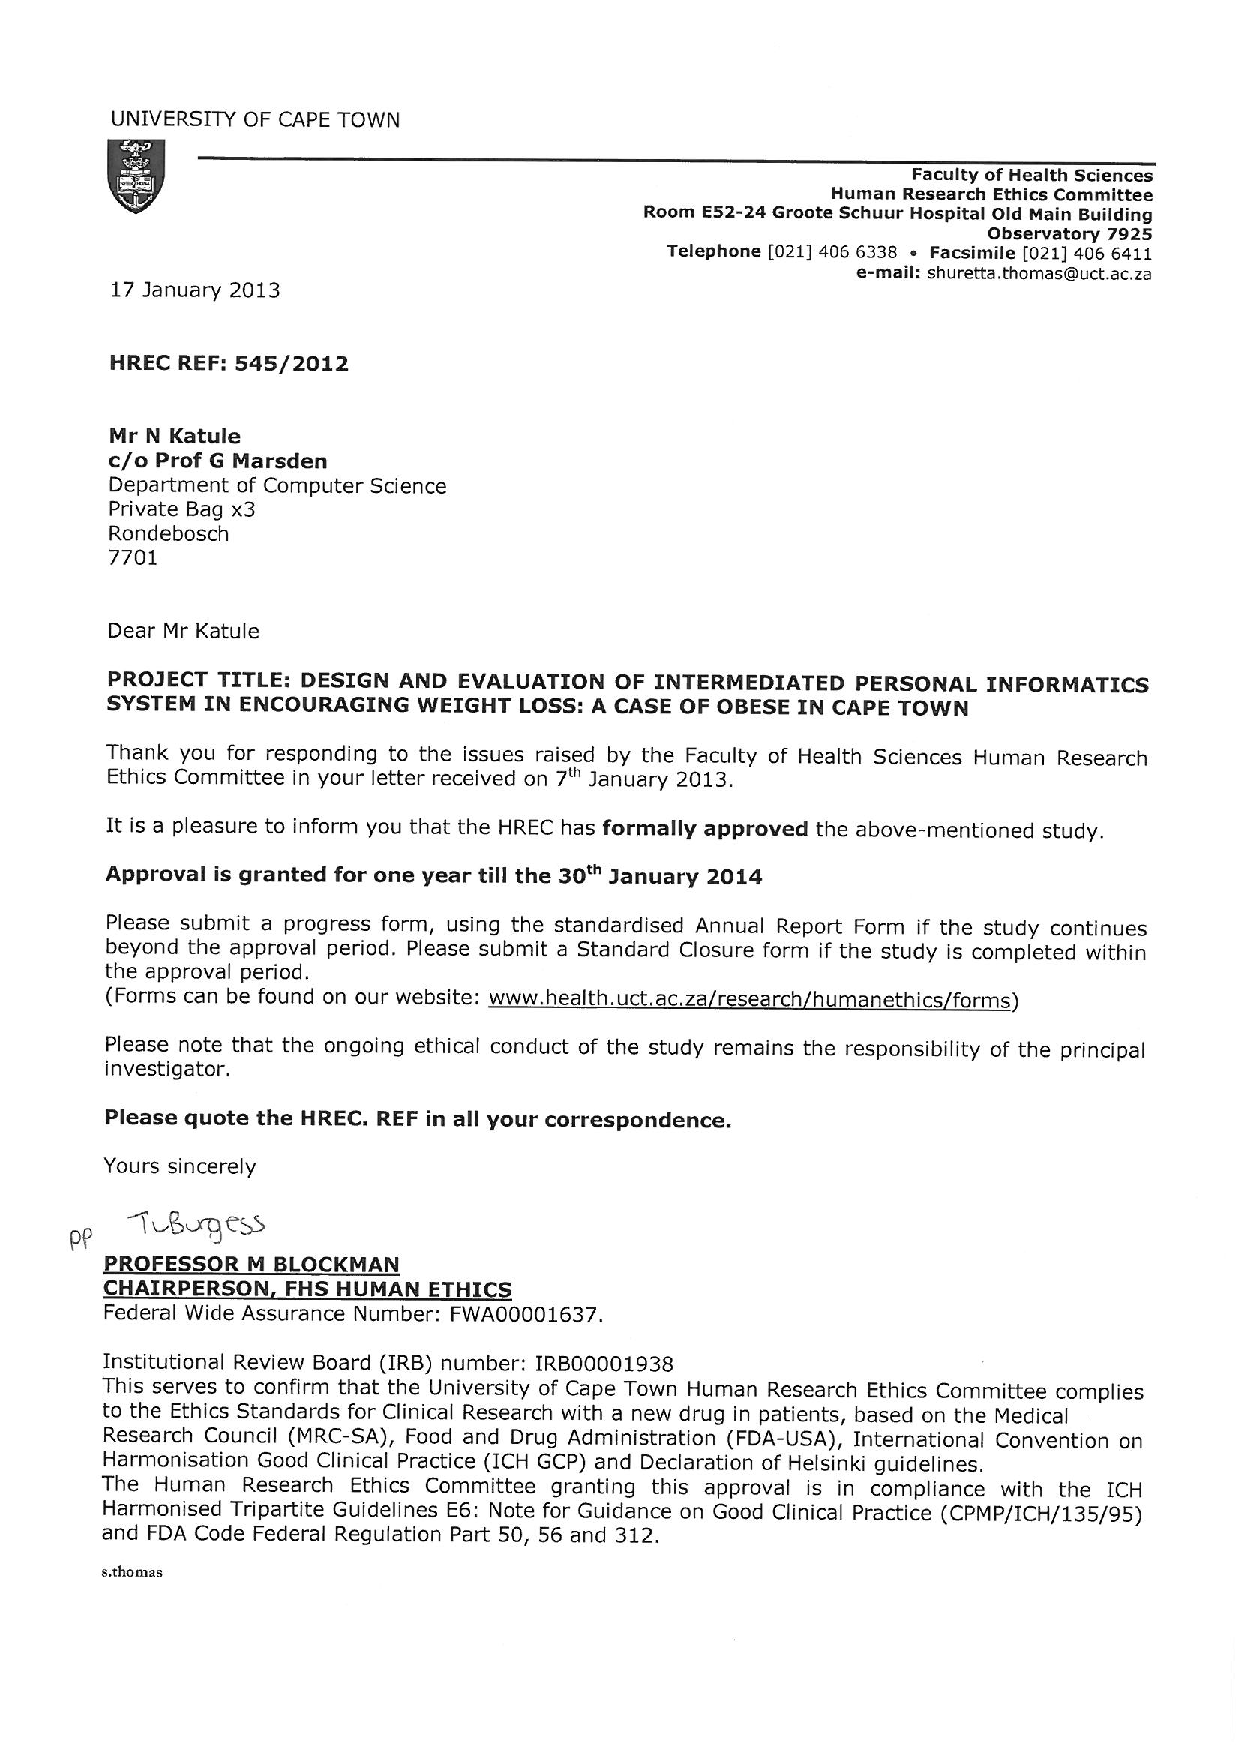
\includepdf[pages=-,pagecommand={},width=\textwidth,offset=90 -20]{Pdfs/fhsrec.pdf}

%\newcommand{\insertrep}[1]{%
%\hspace{-2.4cm}
%\fbox{\includegraphics[page=1,scale=0.8]{#1}}
%\includegraphics[page=1,scale=0.8]{#1}
%\includepdf[scale=0.75,pages=1,frame]{#1}
%}

%\subsection{Interesting Letter}
%\insertrep{Pdfs/baseline_ben.pdf}
%\begin{center}
%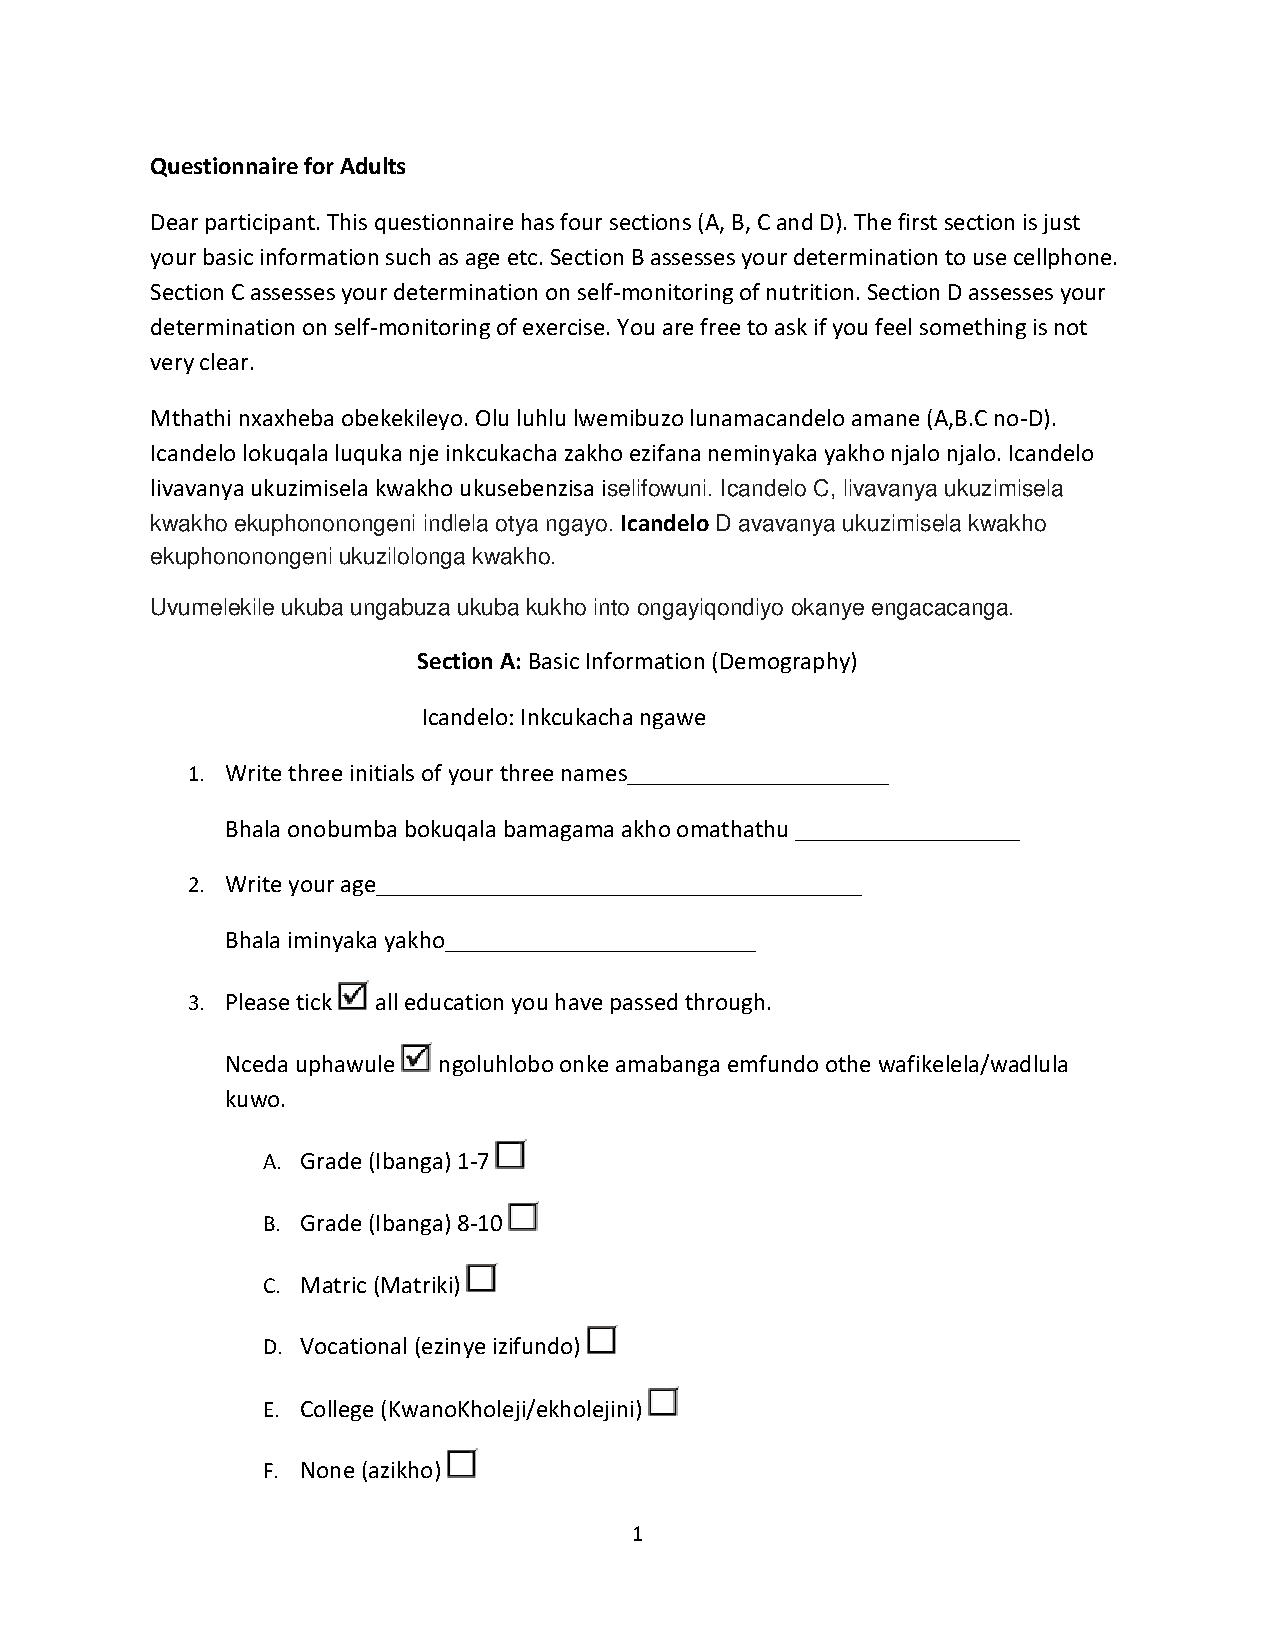
\includepdf[pagecommand={},scale=0.9]{Pdfs/baseline_ben.pdf} 
%\end{center}

%% Appendix A

\chapter{Appendix B. Ethics Approval -- Faculty of Science} % Main appendix title
\clearpage
\label{AppendixB} % For referencing this appendix elsewhere, use \ref{AppendixA}

\lhead{Appendix B. \emph{Ethics Approval -- Faculty of Science}} % This is for the header on each page - perhaps a shortened title

\includepdf[pages=-,pagecommand={},width=\textwidth,offset=90 0]{Pdfs/fsrec.pdf}

%\newcommand{\insertrep}[1]{%
%\hspace{-2.4cm}
%\fbox{\includegraphics[page=1,scale=0.8]{#1}}
%\includegraphics[page=1,scale=0.8]{#1}
%\includepdf[scale=0.75,pages=1,frame]{#1}
%}

%\subsection{Interesting Letter}
%\insertrep{Pdfs/baseline_ben.pdf}
%\begin{center}
%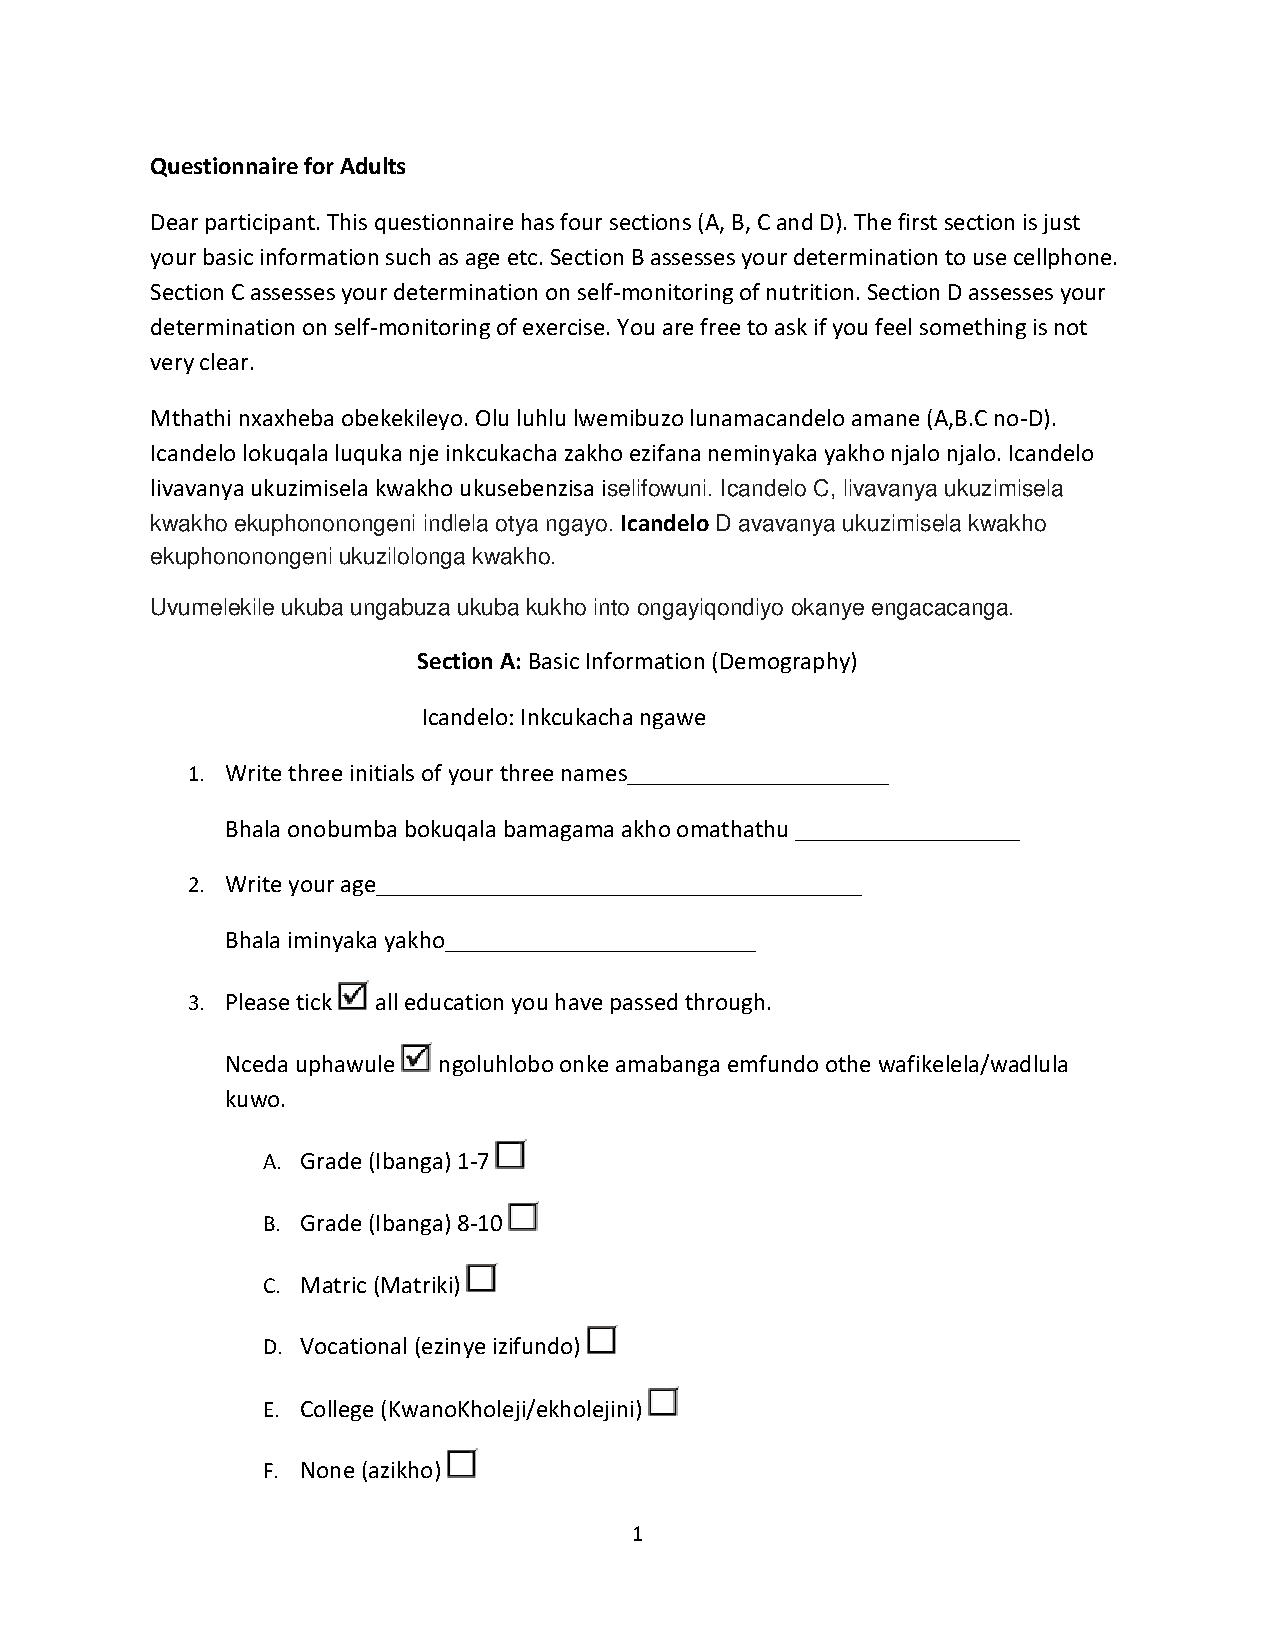
\includepdf[pagecommand={},scale=0.9]{Pdfs/baseline_ben.pdf} 
%\end{center}

% Appendix A

\chapter{Appendix C. Baseline Questionnaires} % Main appendix title
\clearpage
\label{AppendixC} % For referencing this appendix elsewhere, use \ref{AppendixA}

\lhead{Appendix C. \emph{Baseline Questionnaires}} % This is for the header on each page - perhaps a shortened title
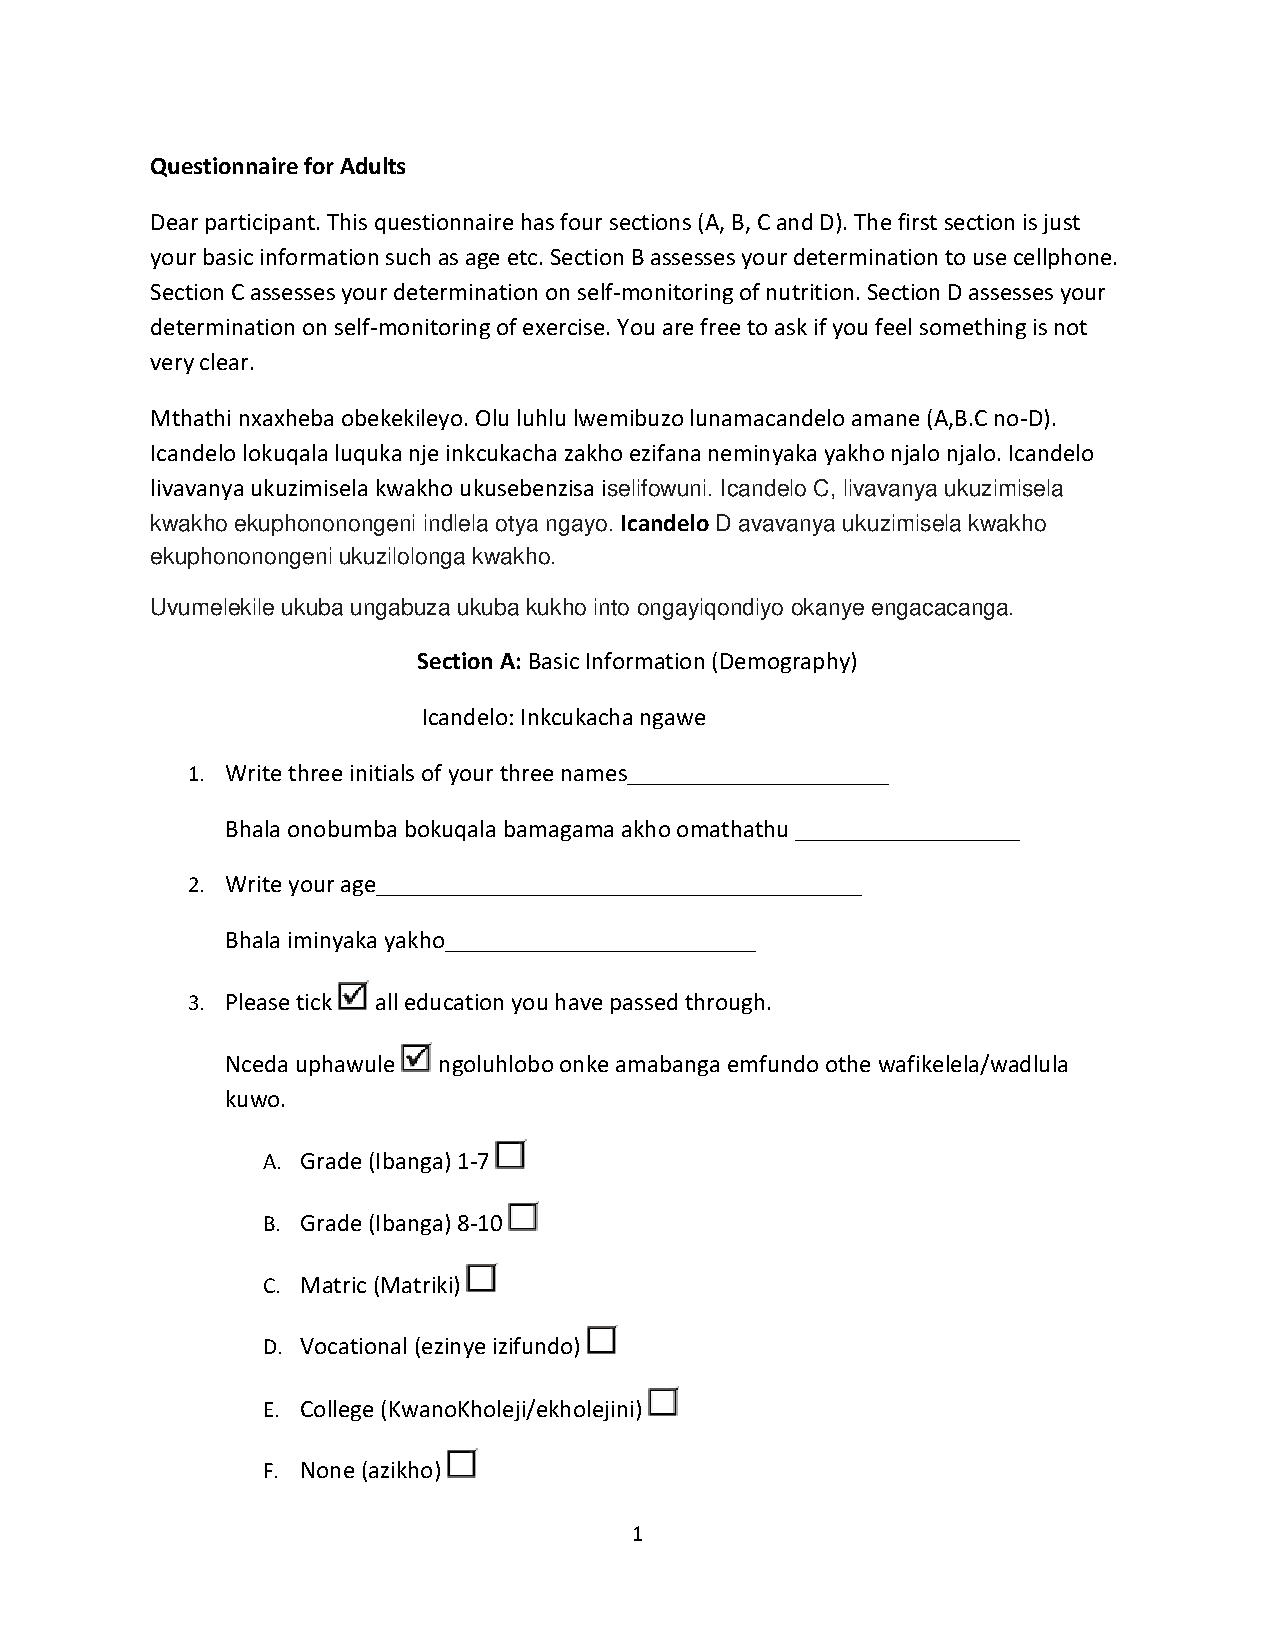
\includepdf[pages=-,frame,pagecommand={},width=\textwidth,offset=90 0]{Pdfs/baseline_ben.pdf}
\clearpage
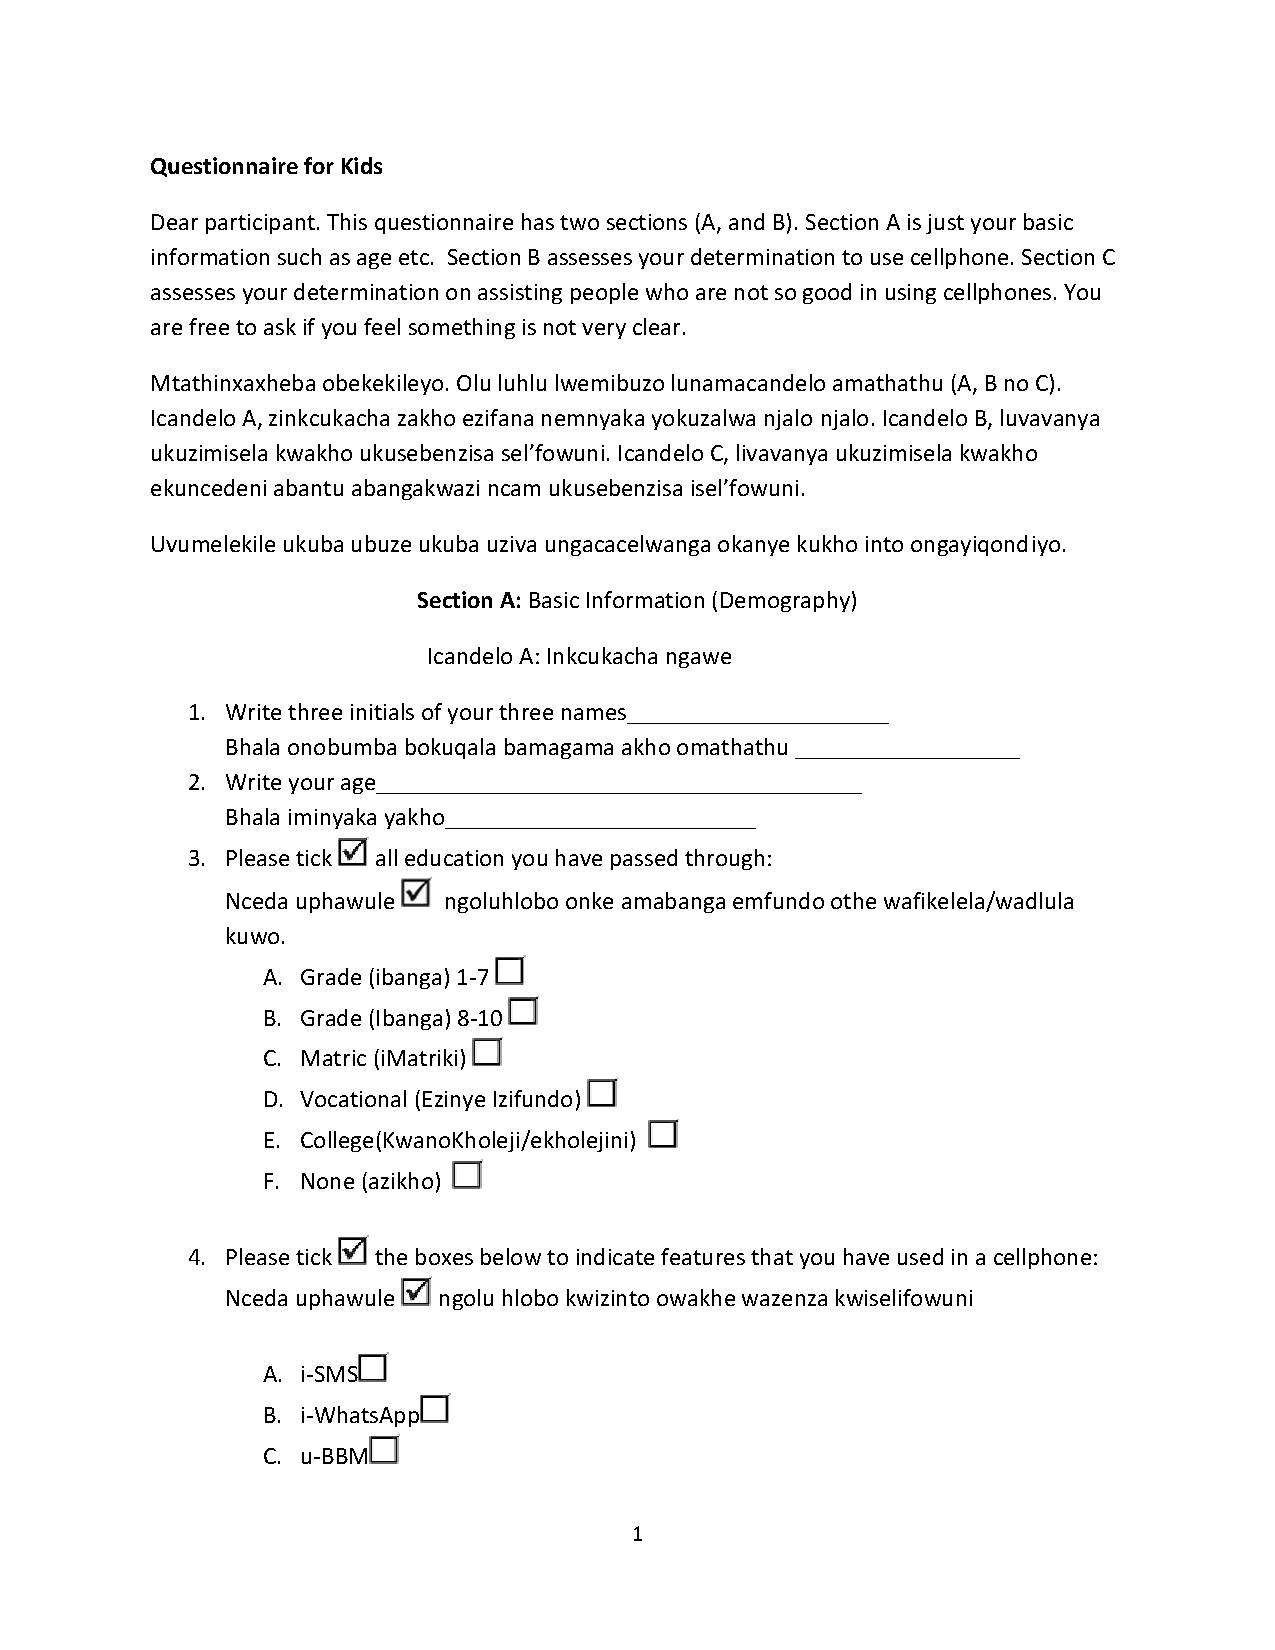
\includepdf[pages=-,frame,pagecommand={},width=\textwidth,offset=90 0]{Pdfs/baseline_interm.pdf}

%\newcommand{\insertrep}[1]{%
%\hspace{-2.4cm}
%\fbox{\includegraphics[page=1,scale=0.8]{#1}}
%\includegraphics[page=1,scale=0.8]{#1}
%\includepdf[scale=0.75,pages=1,frame]{#1}
%}

%\subsection{Interesting Letter}
%\insertrep{Pdfs/baseline_ben.pdf}
%\begin{center}
%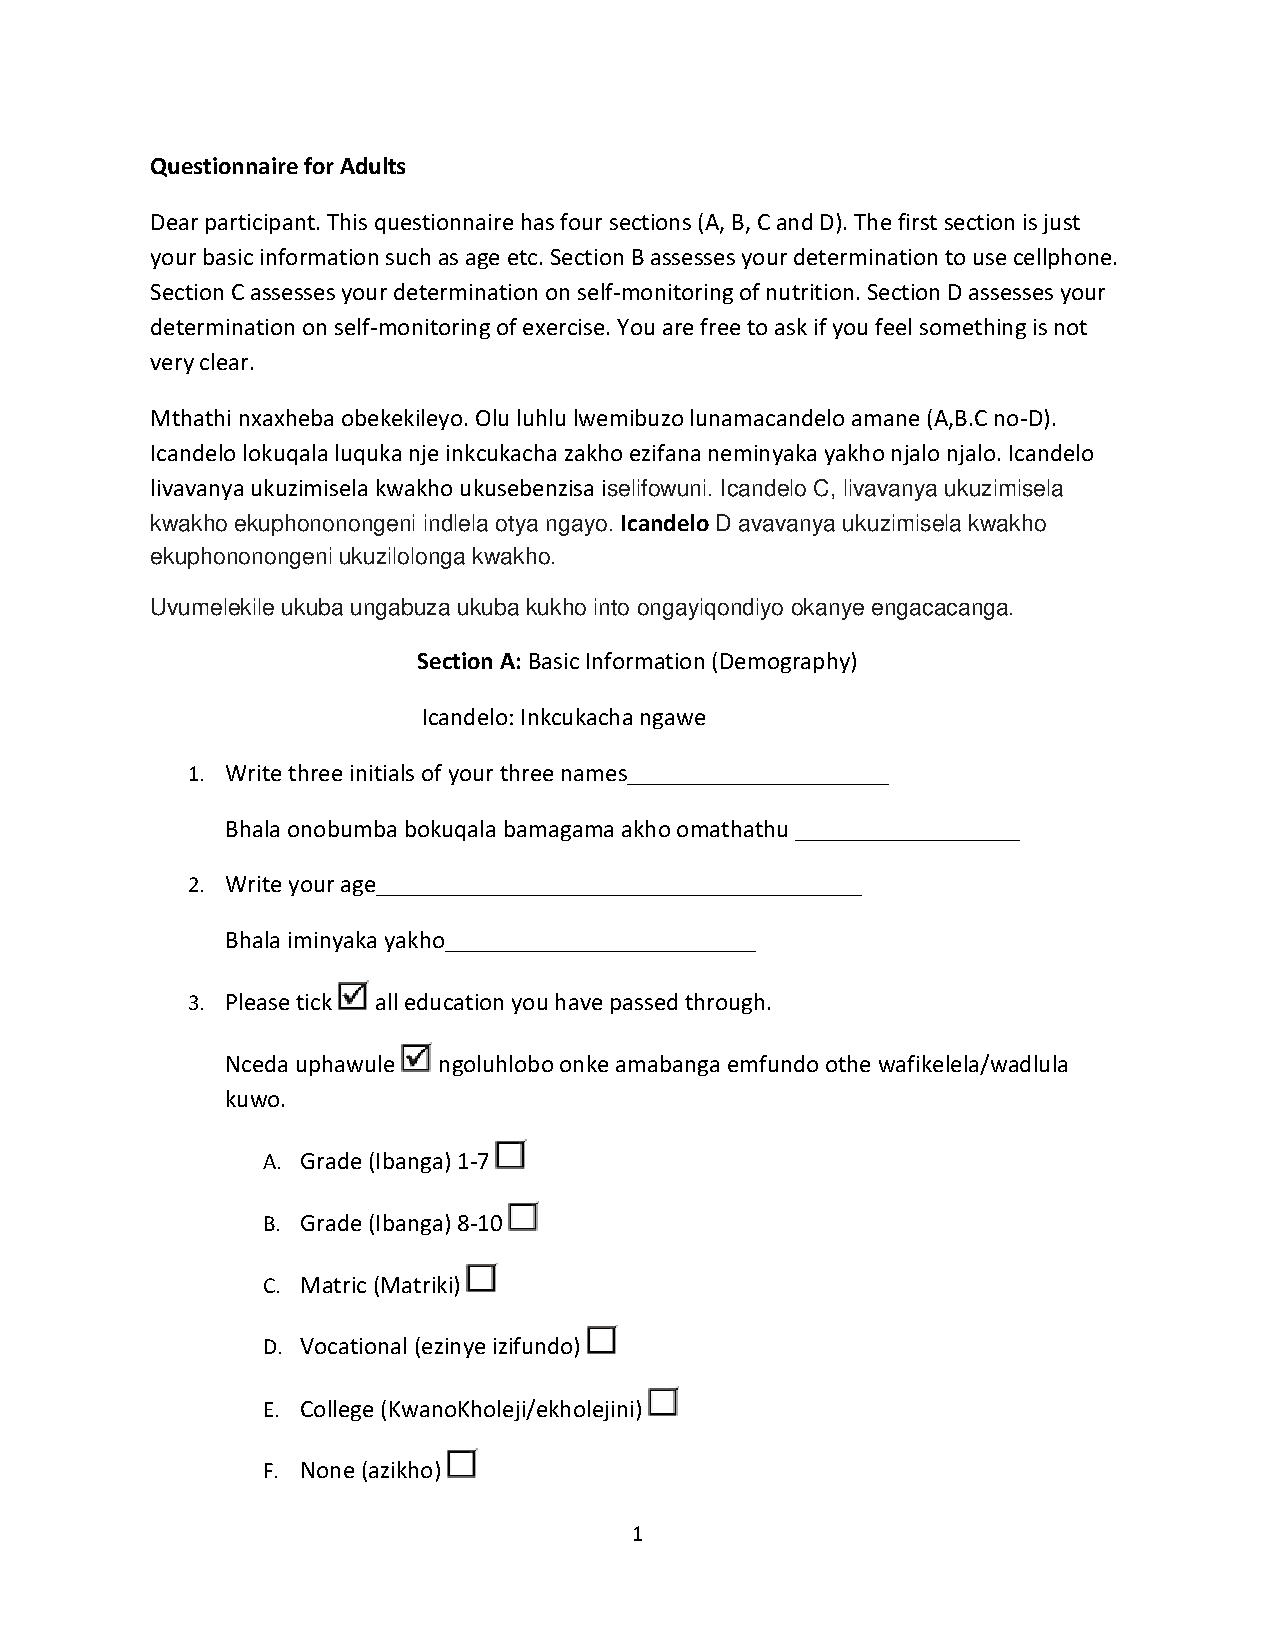
\includepdf[pagecommand={},scale=0.9]{Pdfs/baseline_ben.pdf} 
%\end{center}

% Appendix A

\chapter{Appendix D. Midpoint and Endpoint Questionnaires} % Main appendix title
\clearpage
\label{AppendixD} % For referencing this appendix elsewhere, use \ref{AppendixA}

\lhead{Appendix D. \emph{Midpoint and Endpoint Questionnaires}} % This is for the header on each page - perhaps a shortened title
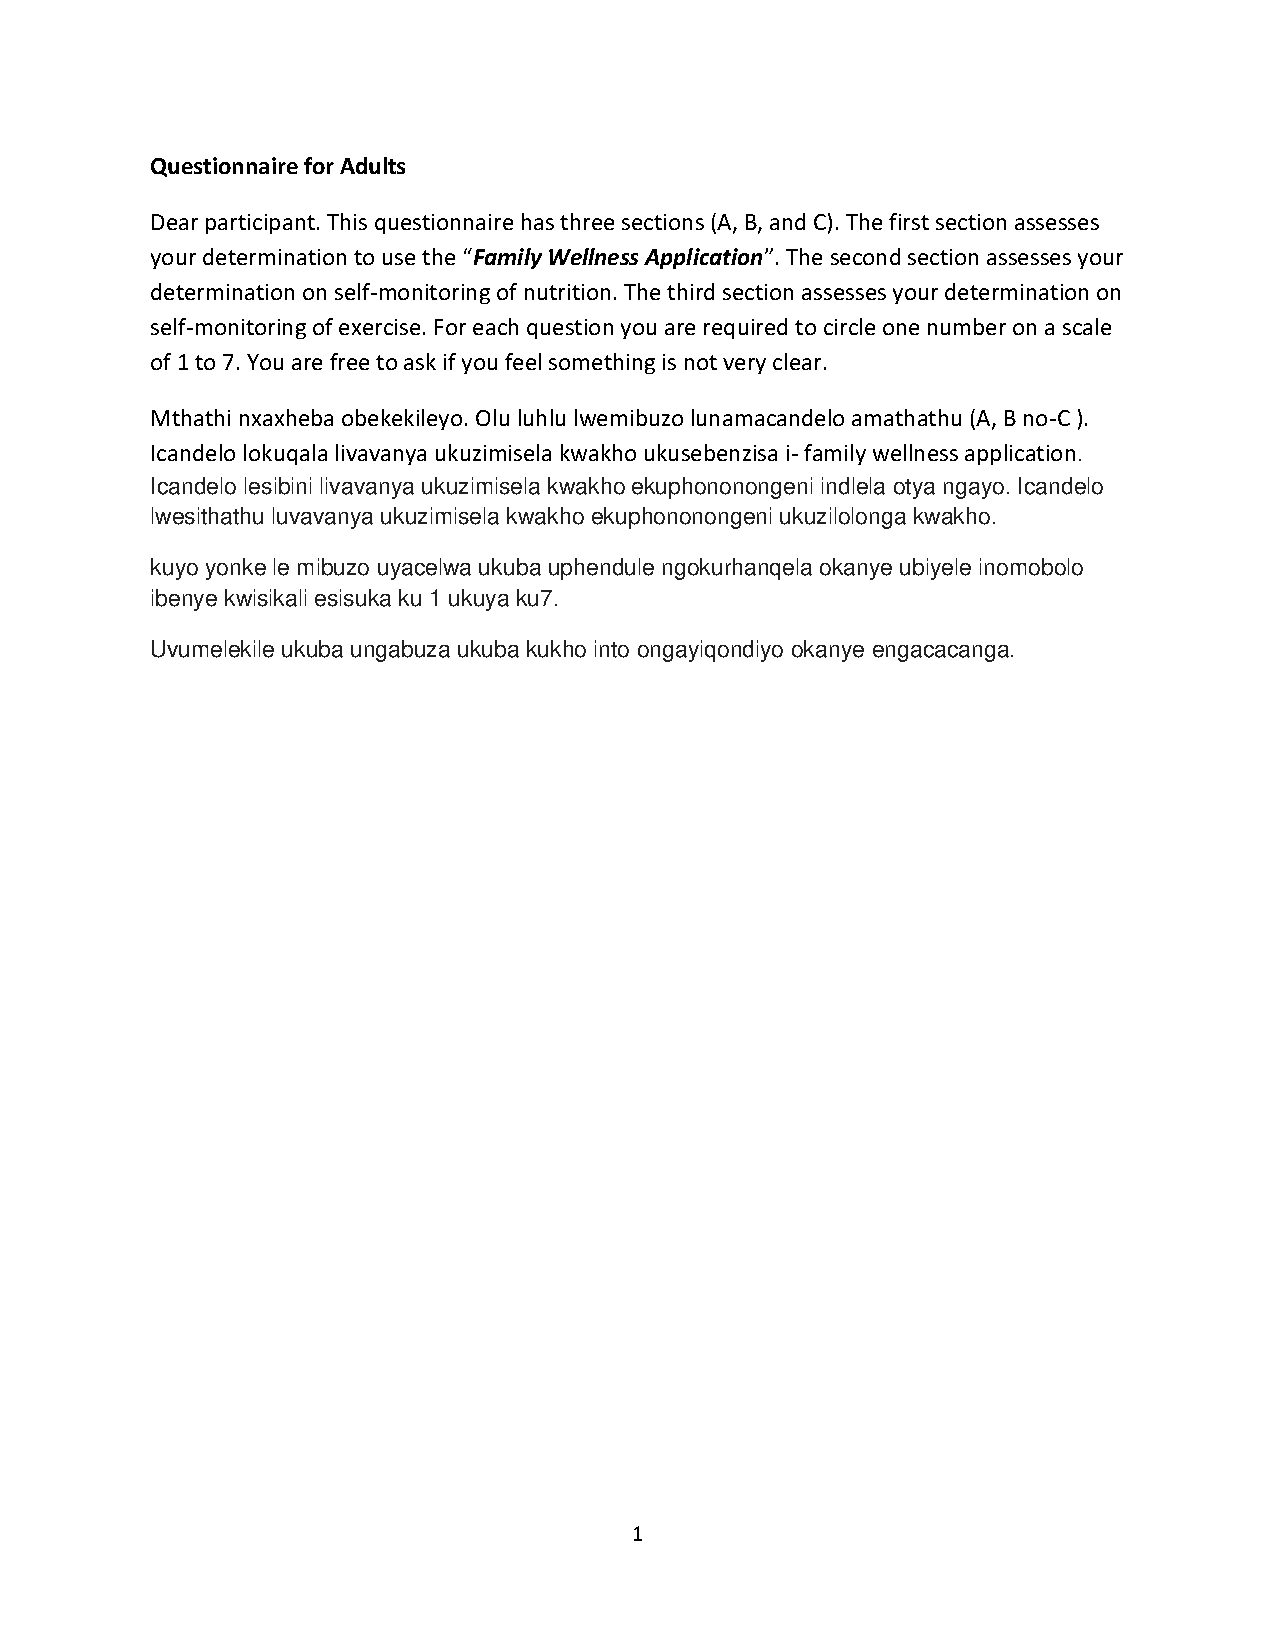
\includepdf[pages=-,frame,pagecommand={},width=\textwidth,offset=90 0]{Pdfs/midpoint_ben.pdf}
\clearpage
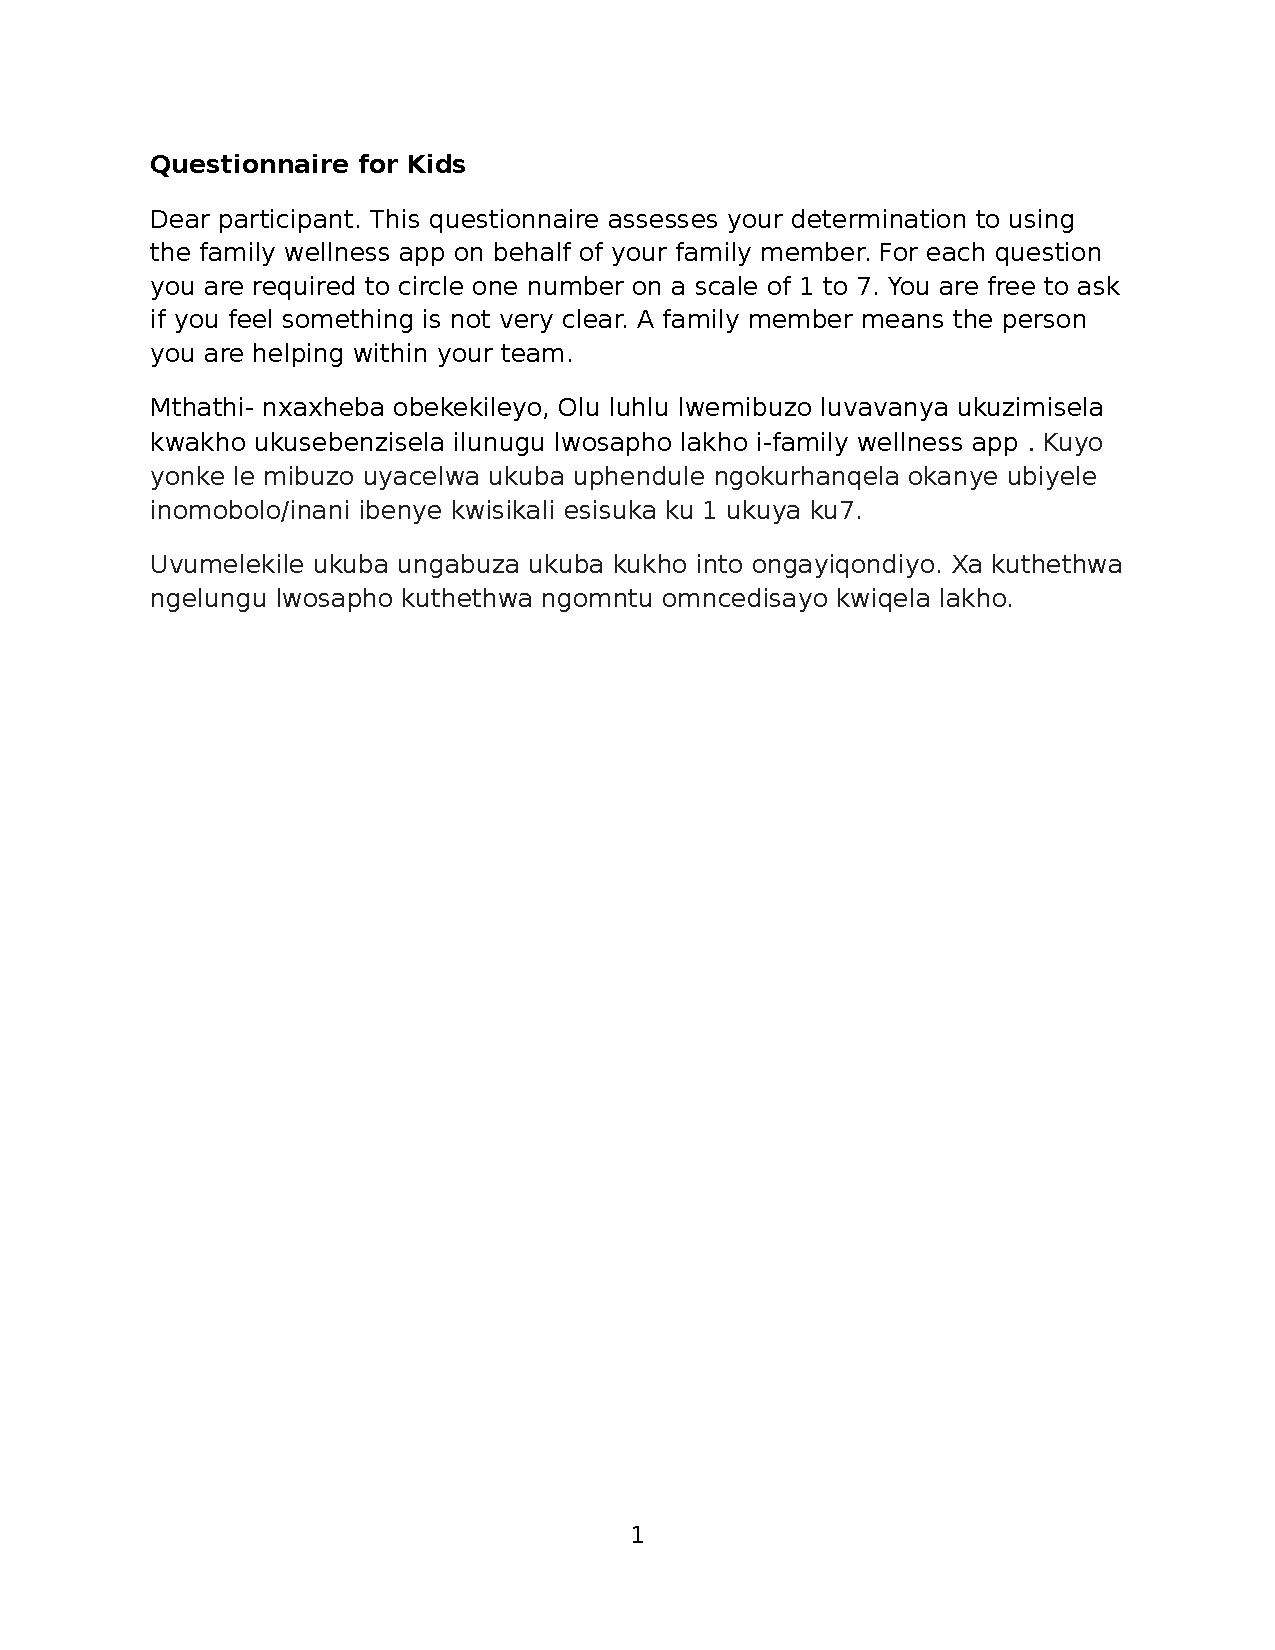
\includepdf[pages=-,frame,pagecommand={},width=\textwidth,offset=90 0]{Pdfs/midpoint_interm.pdf}

%\newcommand{\insertrep}[1]{%
%\hspace{-2.4cm}
%\fbox{\includegraphics[page=1,scale=0.8]{#1}}
%\includegraphics[page=1,scale=0.8]{#1}
%\includepdf[scale=0.75,pages=1,frame]{#1}
%}

%\subsection{Interesting Letter}
%\insertrep{Pdfs/baseline_ben.pdf}
%\begin{center}
%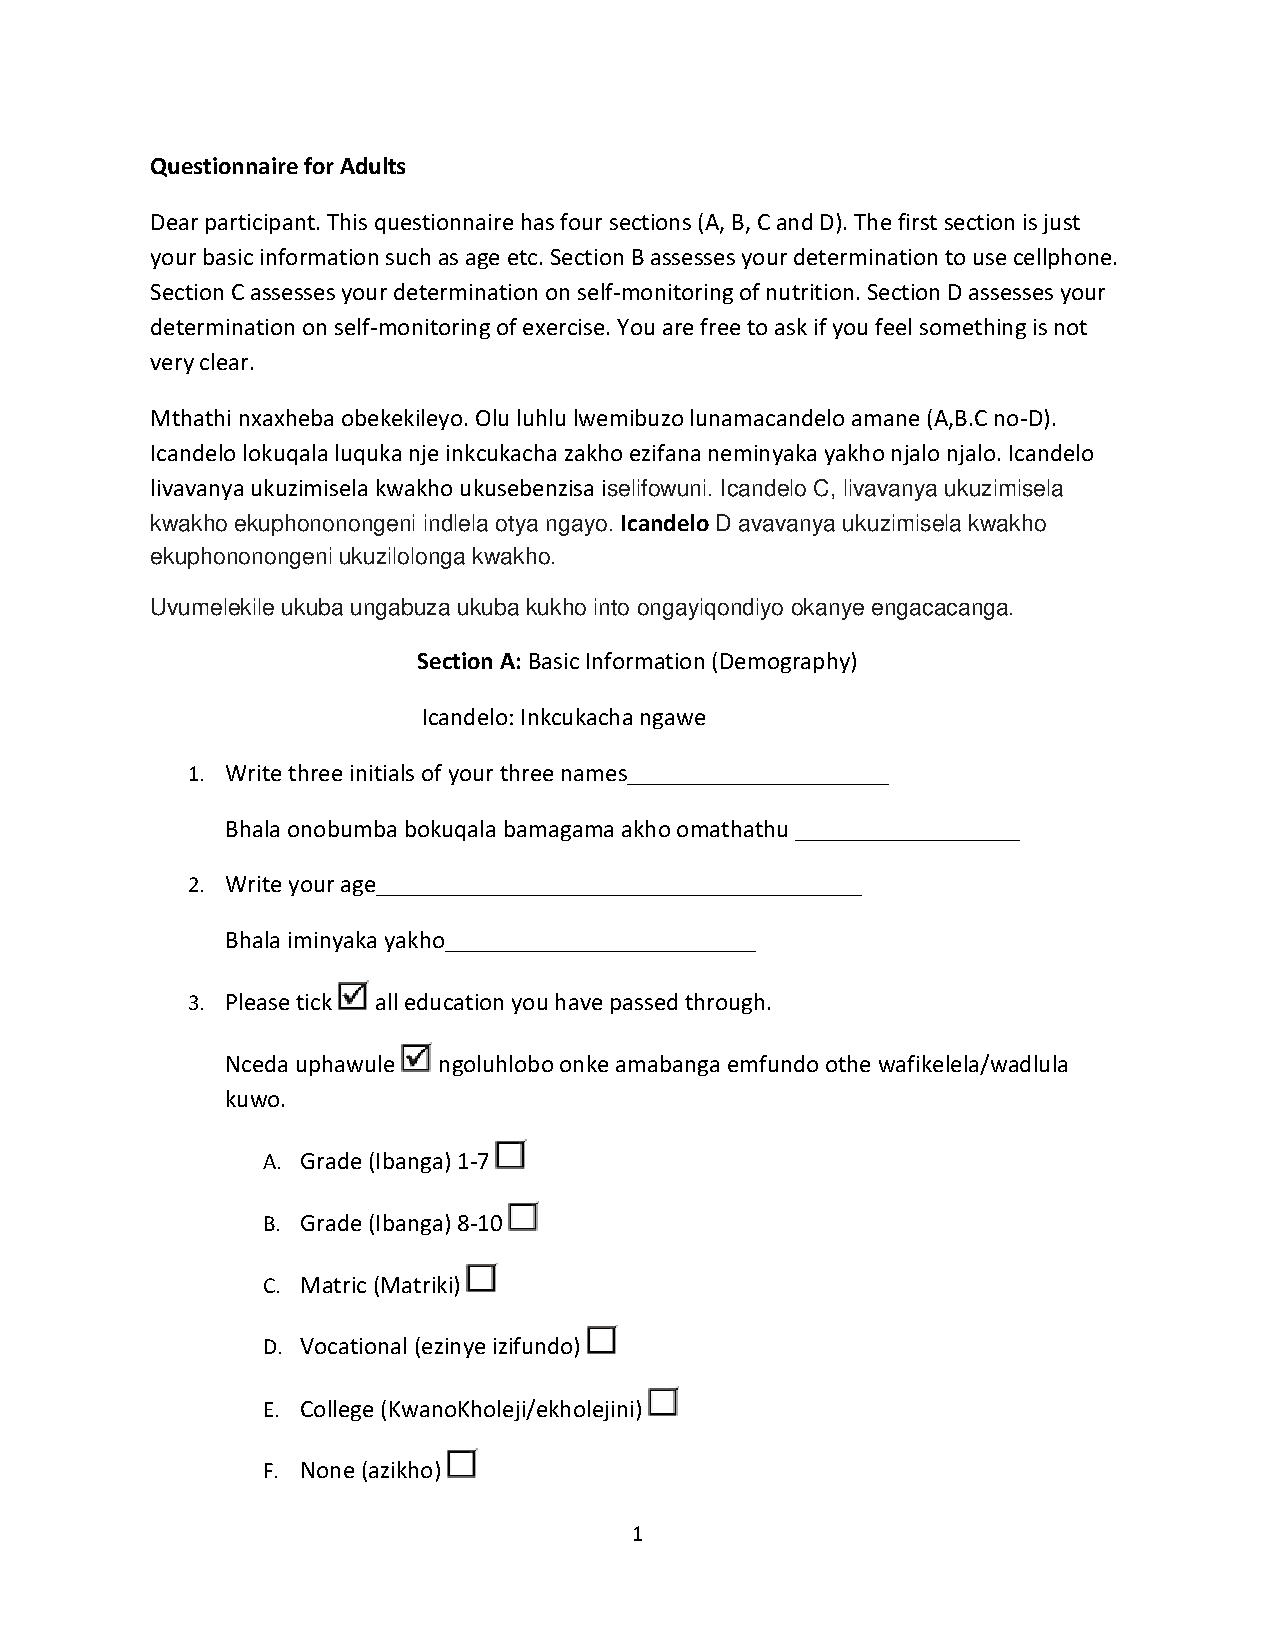
\includepdf[pagecommand={},scale=0.9]{Pdfs/baseline_ben.pdf} 
%\end{center}

\addtocontents{toc}{\vspace{2em}} % Add a gap in the Contents, for aesthetics\textbf{}

\backmatter

%----------------------------------------------------------------------------------------
%	BIBLIOGRAPHY
%----------------------------------------------------------------------------------------

\label{Bibliography}

\lhead{\emph{Bibliography}} % Change the page header to say "Bibliography"

\bibliographystyle{unsrtnat} % Use the "unsrtnat" BibTeX style for formatting the Bibliography
%\bibliographystyle{apa}
%\bibliographystyle{apacite}
\bibliographystyle{apalike}
\bibliography{Bibliography} % The references (bibliography) information are stored in the file named "Bibliography.bib"

\end{document}  